% LTeX: language=fr

\documentclass[a4paper, 12pt]{book}
\usepackage[a4paper, top=3.5cm, bottom=4.0cm, left=3.0cm, right=3.0cm, marginparwidth=2cm]{geometry}
\usepackage[colorlinks=true, allcolors=black]{hyperref}


\usepackage[french]{babel}
\usepackage[T1]{fontenc}
\usepackage[utf8]{inputenc}

\usepackage{enumitem}
\usepackage{float}
\usepackage{standalone}


\usepackage{fancyhdr}
\pagestyle{fancy}
\renewcommand{\headrulewidth}{0pt}
\renewcommand{\footrulewidth}{0pt}

\fancypagestyle{frontmatter}{
    \fancyhf{}
    \fancyfoot[C]{\thepage}
}
\fancypagestyle{body}{
    \fancyhead[LE,RO]{\footnotesize \leftmark}
    \fancyhead[LO,RE]{\footnotesize \rightmark}
    \fancyfoot[C]{\thepage}
}

\makeatletter
\renewcommand\frontmatter{
    \cleardoublepage
    \pagestyle{frontmatter}
    \@mainmatterfalse
}
\renewcommand\mainmatter{
    \cleardoublepage
    \pagestyle{body}
    \@mainmattertrue
}
\makeatother


\makeatletter
\newsavebox\Diam@nd \newlength\x@D\newlength\y@D
\newcommand\quem{
  \sbox\Diam@nd{\raisebox{-1ex}{\scalebox{0.7}[0.9]{\rotatebox{45}{\rule{1em}{1em}}}}}
  \makebox[\wd\Diam@nd]{\makebox[0pt]{\usebox\Diam@nd}\makebox[0pt]{\raisebox{-0.02cm}{\textcolor{white}{?}}}}}
\makeatother


\usepackage{tikz}
\usetikzlibrary{calc}
\usetikzlibrary{patterns}

\usepackage{xcolor}
\definecolor{nrbdarkblue}{RGB}{0,47,81}
\definecolor{nrbmiddleblue}{RGB}{0,124,180}
\definecolor{nrblightblue}{RGB}{79,169,209}
\definecolor{nrbred}{RGB}{215,25,27}
\definecolor{nrbgray}{RGB}{91,96,105}

\newcommand{\rothead}[1]{\rotatebox{45}{#1}}
\newcommand{\oui}{\textcolor{blue!65}{\textbf{$\times$}}}
\newcommand{\non}{\textcolor{red!65}{\textbf{$\times$}}}

\setlength{\parskip}{1em}
\setlist[itemize]{itemsep=0.1cm}

\tikzstyle{incolore} = [rectangle, text centered, minimum height=0.8cm, text width=6.5cm]
\tikzstyle{todo} = [rectangle, fill=gray!50, minimum height=0.4cm, anchor=west]
\tikzstyle{done} = [todo, fill=blue!65]
\tikzstyle{hold} = [rectangle, minimum height=0.4cm, pattern color=blue!65, pattern=north east lines, anchor=west]
\tikzstyle{doing} = [todo, fill=red!65]

\usepackage{mdframed}
\newmdenv[topline=false, bottomline=false, rightline=false, skipabove=\topsep, skipbelow=\topsep, linewidth=0.1cm, linecolor=nrbmiddleblue]{customquote}
\newmdenv[topline=false, bottomline=false, rightline=false, skipabove=\topsep, skipbelow=\topsep, linewidth=0.1cm, linecolor=nrbred]{example}










\begin{document}

\begin{titlepage}
    \newgeometry{top=3cm,bottom=0cm,right=0cm,left=0cm}
    \begin{center} \begin{tikzpicture}
        \node () [text width=10cm, anchor=west] at (-2,5.5) {\noindent \LARGE \textbf{Haute école de Namur Liège Luxembourg}};
        \node () [text width=10cm, anchor=west] at (-2,4.15) {\noindent \large Implantation IESN -- Sécurité des systèmes};
        \node () [anchor=west] at (8,5) {
\includegraphics[width=4cm]{images/logos/LogoHenallux.PNG}};


        \node () [text width=16cm, text centered] at (5,-3) {\LARGE
            Étude et implémentation de solutions pour \\[0.2cm] l'analyse forensique en entreprise
        };
        \node () [text width=16cm, text centered] at (5,-5) {\large
            Grégoire Roumache
        };


        \node () [text width=16cm, text centered] at (5,-11) {
            Travail de fin d’études présenté en vue de l’obtention du diplôme de bachelier en \\ sécurité des systèmes
        };
        \node () [text width=4.5cm, text centered] at (-0.5,-13) {Maître de stage \\ Arnaud Rosette};
        \node () [] at (5,-13) {
\includegraphics[width=6cm]{images/logos/nrb-group.png}};
        \node () [text width=4.5cm, text centered] at (10.5,-13) {Promoteur \\ Christophe Debut};
        \node () [] at (5,-15) {Année académique 2021-2022};
    \end{tikzpicture} \end{center}

    \begin{tikzpicture}[remember picture,overlay]
        \fill[nrbdarkblue] ($(current page.south west)+(0,0)$) rectangle ($(current page.south west)+(4.2,0.25)$);
        \fill[nrbmiddleblue] ($(current page.south west)+(4.2,0)$) rectangle ($(current page.south west)+(8.4,0.25)$);
        \fill[nrblightblue] ($(current page.south west)+(8.4,0)$) rectangle ($(current page.south west)+(12.6,0.25)$);
        \fill[nrbred] ($(current page.south west)+(12.6,0)$) rectangle ($(current page.south west)+(16.8,0.25)$);
        \fill[nrbgray] ($(current page.south west)+(16.8,0)$) rectangle ($(current page.south west)+(21,0.25)$);
    \end{tikzpicture}
\end{titlepage}



\let\cleardoublepage\clearpage





\frontmatter





% LTeX: language=fr

\chapter*{Remerciements} \addcontentsline{toc}{chapter}{Remerciements}

Je souhaite adresser mes remerciements les plus sincères à mon maître de stage Arnaud Rosette qui m'a accompagné et aidé au long de ce stage et sans qui ce stage n'aurait pas été possible.

Ensuite, je tiens à remercier Christophe Debut pour sa lecture attentive de mes rapports de stage tout au long de ces quatre mois de stage.

Je remercie également toute l'équipe SecOps de NRB pour leur disponibilité, leur bienveillance et leur accueil.

Merci à mes parents pour leur soutien, leurs encouragements et leur aide lors de la mise en forme de ce travail.




\tableofcontents \addcontentsline{toc}{chapter}{Table des matières} \newpage


% LTeX: language=fr

\chapter*{Synopsis} \addcontentsline{toc}{chapter}{Synopsis}

"Chaque crime laisse une trace", ce principe a été énoncé par Edmond Locard, pionnier de la police scientifique à une époque où l'informatique n'existait pas. Et pourtant, il s'applique également à ce domaine parce que chaque acteur dans un système informatique laisse une trace de son passage. L'étude du comportement des acteurs malveillants sur un système et l'obtention des indicateurs de compromission (\textit{Indicator of Compromise} ou \textit{IoC} en anglais) est essentiel pour déterminer l'étendue d'une attaque informatique et y mettre fin.

L'objectif de ce travail est de participer à l'amélioration de la détection et de l'analyse des menaces dans l'entreprise. Pour arriver à cela, mon travail s'est focalisé sur la recherche d'un ensemble d'outils, la conception et l'implémentation d'une solution et des procédures d'acquisition et d'analyse forensique.

La première section de ce travail est consacrée à l'analyse comparative des outils. La combinaison de la recherche théorique et de l'expérimentation pratique ont permis de sélectionner les outils les plus appropriés sur base d'une liste de besoins.

La deuxième section de ce travail se concentre sur la conception et l'implémentation d'une solution. Son architecture a été conçue pour prévenir la propagation des menaces afin de pouvoir l'utiliser sans augmenter les risques pour l'entreprise. Elle comporte notamment une sandbox pour analyser des logiciels malveillants mais aussi des outils d'analyse de la mémoire volatile et non-volatile permettant de montrer la présence, l'exécution et l'origine d'un logiciel malveillant.

La troisième section de ce travail est dédiée aux procédures. Elles ont été travaillées en se basant sur celles utilisées par des institutions privées comme publiques tout en les adaptant au contexte de l'entreprise.

Enfin, des pistes d'amélioration sont envisagées et notamment après avoir utilisé cette solution dans des cas réels.





% LTeX: language=fr

\chapter*{Présentation de l'entreprise} \addcontentsline{toc}{chapter}{Présentation de l'entreprise}

\textit{Network Research Belgium}, souvent abrégé sous la forme du sigle \textit{NRB} est une entreprise belge du secteur des TIC, les technologies de l'information et de la communication, fondée en 1987 en Belgique, mais à vocation européenne. L'entreprise fournit des services dans les quatre domaines suivants:
\begin{itemize}
    \item la \textit{consultance} pour accompagner ses clients dans leurs démarches de transformation numérique et le conseil en cybersécurité;
    \item les \textit{services logiciels} comme le développement et la maintenance d'applications;
    \item les \textit{services infrastructures et clouds}, NRB permet à ses clients d'utiliser le cloud privé de NRB et les clouds publics d'IBM, Microsoft, Google et Amazon;
    \item les \textit{services de managed staffing} consistent à fournir du personnel à des entreprises qui en ont besoin pour conduire à bien leurs projets.
\end{itemize}

Certains de ces services sont fournis par les filiales du groupe NRB. En effet, NRB est un groupe qui s'agrandit notamment par des acquisitions d'entreprises dans le domaine technologique. En 2020, le groupe NRB comptait 3200 collaborateurs, avec un chiffre d'affaires de 413 millions d'euros.

Au sein de NRB, il y a l'équipe SecOps où j'ai réalisé mon stage. SecOps vient de \textit{Sécurité et Opérations}, c'est l'équipe principale de gestion de la sécurité chez NRB. Comme l'indique le mot \textit{sécurité} de SecOps, ils doivent gérer les incidents de sécurité qui se produisent dans l'entreprise et chez certains de leurs clients mais ils ne gèrent pas l'ensemble des \textit{opérations}. Par exemple, ce n'est pas leur rôle de conduire un changement réseau du début à la fin, c'est le rôle de l'équipe réseau. Cependant, ils ont la responsabilité de vérifier que ce changement ne comporte pas de risque de sécurité important.







\mainmatter





% LTeX: language=fr

\chapter{Introduction}

Ce projet participe à l'amélioration de l'analyse des menaces et des données forensiques dans l'entreprise. Afin d'y parvenir, ce travail commence par une analyse des besoins et une révision des concepts théoriques associés au processus de réponse à incident pour avoir une vue d'ensemble des processus. S'ensuit la recherche et la comparaison d'un ensemble d'outils afin de les sélectionner sur base de critères objectifs.

Après avoir sélectionné un nombre de logiciels et avoir revu les concepts théoriques, vient la conception de l'architecture d'une solution d'analyse de données forensiques, qui est isolée autant que possible afin de prévenir la propagation des menaces. Son implémentation est également abordée, ainsi qu'une réflexion sur son utilisation, mais aussi sur les procédures d'acquisition et d'analyse forensique et de menaces.

Le sujet abordé étant vaste, il est impossible de le couvrir dans son entièreté. Ce travail offre, bien qu'il ait rempli les objectifs initiaux, de nombreuses possibilités d'amélioration et de sujets à approfondir. Ces pistes d'amélioration et sujets à approfondir seront donc aussi envisagés.




% LTeX: language=fr

\chapter{Analyse des besoins}

L'analyse des besoins sert à poser un cadre à un projet. Après avoir déterminé les attentes, on peut chercher à lister les étapes qu'il faudra pour achever le projet et faire une estimation du temps et des coûts pour y arriver. Ensuite vient une phase de discussion où toutes les parties impliquées dans le projet se mettent d'accord sur les moyens mis à dispositions et les besoins qui devront être satisfaits ou non. Il est important de revenir dans le courant de l'implémentation du projet sur les points bloquants afin de les résoudre

Afin d'améliorer les capacités de l’équipe SecOps en termes d’analyse forensique, ce qui comprend aussi l’analyse de menaces, le besoin était de créer une solution d'analyse isolée. Elle doit être isolée pour prévenir la propagation des menaces analysées, mais elle doit aussi pouvoir être facilement restaurée dans un état vierge. Parmi ses outils, elle doit compter un ensemble d'outils d'analyse forensique et d'analyse de menaces, y compris une sandbox, des outils d'analyse réseau, des logiciels de copie et de montage de disque, etc. Le tout avec une documentation sur l'utilisation des outils.

Pour remplir les objectifs de restauration facile de l'état de la machine et isoler au mieux les machines d'analyse, il a été décidé que celles-ci seraient installées dans un environnement virtualisé cloud. Pour des raisons de coût, elle se trouvera non pas dans un cloud public, mais dans NECS, le cloud privé de NRB.

Parce que certains des outils à installer ne fonctionnent que sur des systèmes de type Linux et d'autres uniquement sur des systèmes de type Windows, il convient d'installer deux machines virtuelles avec chacune un de ces deux systèmes. De plus, la solution de sandbox nécessite que la virtualisation imbriquée soit activée sur la machine virtuelle qui la supporte afin de pouvoir lancer des machines virtuelles imbriquées dans lesquelles le logiciel ou document malveillant va être détonné.

Le dernier besoin qui n'a pas encore été abordé est celui de l'acquisition des données forensiques. Il s'agit non-seulement de pouvoir obtenir les données forensiques d'une machine Windows, mais aussi de pouvoir acquérir les données forensiques provenant de clés USB.





% LTeX: language=fr

\chapter{Concepts théoriques}










\section{Réponse à incident}


Le NIST, le \textit{National Institute of Standards and Technology} aux États-Unis, définit un \textit{incident de cybersécurité} ainsi: \cite{1}

\begin{customquote}
    \itshape Un évènement de cybersécurité dont on a déterminé qu'il avait un impact sur l'organisation provoquant le besoin d'une réponse et d'une restauration.
\end{customquote}

Pour illustrer cette définition, on peut imaginer un acteur malintentionné souhaitant infecter une entreprise avec un logiciel malveillant appelé, \textit{malware}, pour lui voler des données confidentielles comme les travaux sur les brevets qui n'ont pas encore été déposés. Pour faire cela, ce \textit{threat actor} va envoyer un mail contenant une pièce jointe infectée à un membre du personnel. Supposons qu'on détecte l'infection immédiatement après que le PC de l'employé ait été compromis, on a:
\begin{enumerate}
    \item Un impact sur l'organisation, un risque que le PC infecté serve de \textit{pont} à l'attaquant pour rentrer dans le réseau interne, étendre son contrôle et voler des informations auxquelles il ne devrait pas avoir accès.
    \item Un besoin de réponse et de restauration pour contenir la menace, l'éradiquer et restaurer les systèmes à leur état initial.
\end{enumerate}

La détection de cet évènement de cybersécurité enclenche un mécanisme de réponse à incident. Un des frameworks de réponse à incident les plus utilisés est celui du NIST qui consiste en quatre phases: \cite{2}
\begin{enumerate}
    \item La \textit{préparation} qui doit bien sûr être réalisée avant que les incidents de sécurité ne surviennent. Il s'agit de prévenir les incidents mais aussi de préparer l'équipe qui les résoudra en lui donnant le matériel dont elle a besoin ainsi que préparer les procédures à suivre lors du moment fatidique. Par exemple, comment communiquer dans le cas d'une attaque ? Il faut éviter de multiplier les moyens de communication pour que l'information ne se perde pas mais aussi chercher à utiliser un canal chiffré et résiliant.
    \item La \textit{détection et l'analyse} des indicateurs de compromission des systèmes informatiques permettent de détecter et prévenir des incidents. C'est un travail d'évaluation et de tri: une équipe en charge de la sécurité dans une entreprise ou une autre institution reçoit beaucoup de signaux dont certains sont des \textit{faux positifs}, c'est-à-dire qu'ils ne représentent pas de réelle menace pour le système informatique. Il revient à l'analyste de corréler les informations et de définir le niveau de réponse à adopter.
    \item Une fois qu'un incident a été déclaré, la phase de \textit{mise sous-contrôle, d'éradication de la menace et de restauration} est enclenchée. La première chose à faire est de choisir la méthode d'endiguement qui va être différence en fonction de la nature de l'incident et des objectifs recherchés (efficacité, disponibilité du service, etc.). Ensuite, il faut récupérer les preuves en faisant de l'acquisition de données forensiques, identifier les attaquants et procéder à la restauration des systèmes en modifiants les mots de passe compromis et en corrigeant les vulnérabilités exploitées.
    \item L'\textit{analyse post-incident} sert à améliorer les procédures utilisées. Par exemple, en déterminant quelles informations auraient dû remonter plus tôt ou qu'est-ce qui a ralenti le rétablissement des systèmes. Cette analyse sert aussi à déterminer les coûts de l'incident en termes de quantité de travail, mais aussi au niveau du temps perdu entre la détection de l'incident et le moment où l'équipe de réponse est intervenue. Grâce aux leçons apprises lors de cette analyse, on peut également améliorer la prévention des incidents pour l'organisation.
\end{enumerate}

\begin{figure}
    \centering
    \noindent
    \makebox[\textwidth]{\includestandalone{images/IR-diagram/ir-diagram}}
    \caption{Framework de réponse à un incident de cybersécurité du NIST.}
    \label{fig:ir-diagram}
\end{figure}

Ce travail de fin d'étude se concentre sur les phases intermédiaires du framework de réponse à incident du NIST ou plus exactement, dans la boucle au centre de la figure \ref{fig:ir-diagram}. L'acquisition des données forensiques et leur analyse se trouvent au cœur de la troisième partie du processus mais les résultats qui en sont tirés peuvent entraîner un retour en arrière sur la phase d'analyse. Un cas typique est lorsqu'en analysant les données forensiques et les malwares, on trouve de nouveaux \textit{IoC}, des \textit{indicators of compromise} ou indicateurs de compromissions en français, on doit alors relancer une recherche pour vérifier que le système informatique n'a pas d'autres machines infectées. Par exemple, si en analysant le malware on trouve une liste d'adresse IP, on pourrait rechercher si d'autres machines du parc informatique ne les ont pas contactées.





\section{Processus forensique}

Comme le définit Interpol, l'organisation internationale de police criminelle: \cite{3}

\begin{customquote}
    \itshape La forensique numérique est la branche de la science forensique qui se concentre sur l'identification, l'acquisition, le traitement, l'analyse et la production de rapport sur les données stockées électroniquement.
\end{customquote}

Bien qu'elle ait été formulée par une organisation qui ne s'occupe pratiquement pas de cybersécurité, cette définition y a toute sa place et le processus d'analyse d'Interpol \cite{4} peut aussi être utilisé dans le monde de l'entreprise même lorsque aucune attaque informatique n'a été perpétrée. Un exemple: si on suspecte un employé de voler des données confidentielles en les transférant de son lieu de travail à son domicile, une investigation forensique peut potentiellement le montrer.

Un des processus les plus utilisés en cybersécurité pour la forensique est celui du NIST qui le divise en quatre étapes: \cite{5}

\begin{enumerate}
    \item Tout d'abord, il faut identifier, labelliser et collecter les données forensiques tout en préservant l'intégrité des données, c'est la phase d'\textit{acquisition}.
    \item Vient ensuite la phase d'\textit{inspection}, lors de laquelle l'enquêteur doit traiter les données, les analyser et extraire les données d'importance.
    \item L'\textit{analyse} va encore plus loin en obtenant les informations à partir des données extraites. C'est à ce moment-là qu'on doit répondre aux questions qui ont poussé à lancer tout ce processus forensique.
    \item Enfin, il faudra créer un \textit{rapport}. En fonction de la situation, on peut y mettre les actions qui restent à prendre, celles déjà effectuées, les outils et procédures utilisés ou des recommandations d'amélioration pour éviter que des incidents similaires ne se reproduisent.
\end{enumerate}

\begin{example}
    \hspace{0.45cm} Par exemple, dans le cas d'un PC infecté par un malware, un analyste forensique devrait:
    \begin{enumerate}
        \item \textit{Acquérir} les données forensiques en faisant une image de la RAM et du disque pour pouvoir les préserver et les analyser. Il faut le faire rapidement pour éviter de perdre des données volatiles (comme les données stockées dans la RAM).
        \item \textit{Inspecter} les données pour en extraire celle qui ont de l'importance. Par exemple: extraire les fichiers contenant les preuves d'exécutions des programmes, les fichiers ouverts récemment, les adresses IP auxquelles le PC s'est connecté, etc.
        \item \textit{Analyser} les données extraites à la phase d'inspection pour récupérer des informations sur les évènements qui nous intéressent. Dans ce cas, identifier le malware, déterminer ce qu'il a fait sur le système, d'où il vient, etc.
        \item Écrire un \textit{rapport} afin d'expliquer les procédures suivies, les résultats d'analyse, les recommandations pour prévenir les incidents similaires dans le futur, etc.
    \end{enumerate}
\end{example}

La manière dont sont manipulées les données forensiques a également une grande importance. L'ACPO (\textit{Association of Chief Police Officers}) a énoncé quatre principes qui doivent être suivis par ceux qui seront en charge d'acquérir, analyser et conserver les données forensiques: \cite{6}
\begin{enumerate}
    \item Aucune action entreprise ne doit modifier les données forensiques.
    \item Si une personne doit accéder aux données originales, elle doit être compétente, savoir expliquer et donner des preuves de chacune de leurs actions.
    \item Une trace de tout ce qui a été effectué doit être créée et conservée. Une personne tierce doit être capable d'examiner la liste des actions réalisées, les réitérer et arriver au même résultat.
    \item La personne en charge de l'enquête est responsable de s'assurer que ces principes et la loi sont bien appliqués.
\end{enumerate}





\section{Processus d'analyse de menace}

Lorsqu'on a réussi à identifier un document malicieux, appelé \textit{maldoc}, ou un logiciel malicieux, appelé \textit{malware}, il faut l'analyser. Pourquoi ? Tout l'intérêt de l'analyse de menaces est de trouver plus d'IoC, des \textit{indicators of compromise} ou indicateur de compromission en anglais. Ce sont des données forensiques qui servent à identifier l'activité d'une menace sur un système informatique.

\begin{example}
    \hspace{0.45cm} Par exemple, dans le cas où un analyste en cybersécurité repère des connexions suspectes à des adresses IP vers des pays auxquelles les machines ne devraient pas se connecter, il va vite bloquer ces adresses IP et lister les machines qui les ont contactées pour pouvoir y lancer des scans anti-virus, modifier les mots de passe des personnes qui étaient connectés sur ces machines, etc.

    L'intérêt de récupérer le malware qui tourne sur le système pour l'analyser est double:
    \begin{itemize}
        \item En faisant l'analyse, il va peut-être trouver des nouvelles adresses IP et de nouveaux domaines malicieux sur lesquels il faudra effectuer une recherche et qu'il faudra bloquer.
        \item Il peut aussi déterminer d'où vient le vecteur d'entrée dans le système informatique: est-ce que la porte d'entrée est un mail de phishing, un document infecté, une vulnérabilité exploitée par un attaquant, etc. En faisant des recherches, un analyste en cybersécurité peut trouver un mot de passe compromis à remplacer d'urgence ou une vulnérabilité à corriger.
    \end{itemize}
\end{example}

L'analyse des malware s'effectue en quatre étapes:
\begin{enumerate}
    \item L'\textit{analyse automatique} au cours de laquelle le malware est analysé de manière automatique par des logiciels comme des anti-virus, des sandboxes ou autre. Certaines menaces avancées peuvent échapper à l'analyse de ces outils et c'est pour ça qu'il faut parfois lancer en une analyse manuelle mais c'est déjà un bon premier pas pour déterminer la dangerosité du logiciel/document et ses capacités en termes de nuisance.
    \item L'\textit{analyse des propriétés statiques} peut permettre de trouver les capacités d'un programme et des IoC. Par exemple, en scannant un programme pour en extraire les chaînes de caractères, on peut trouver des adresses IP, des noms de domaines ou des adresses de compte bitcoin.
    \item L'\textit{analyse interactive du comportement} consiste à lancer le malware dans un débogueur pour pouvoir voir en temps réel ce qu'il fait mais aussi pouvoir contourner les mécanismes anti-analyse qui sont parfois inclus dans les malwares pour rendre la tâche plus difficile aux analystes.
    \item La \textit{rétro-ingénierie manuelle} (\textit{manual reverse engineering} en anglais) est l'étape la plus difficile et rarement exécutée par l'analyste. Il s'agit de prendre le code compilé, et parfois obfusqué par le développeur de malware pour rendre la rétro-ingénierie encore plus difficile.
\end{enumerate}





\section{Fonctionnement des outils}



\subsection{Acquisition de la mémoire volatile}

Pour commencer cette section, voici la définition de ce que sont les données volatiles d'après le NIST: \cite{5}

\begin{customquote}
    Les données volatiles sont les données d'un système qui sont perdues après que l'alimentation de l'ordinateur soit coupée ou dû au passage du temps. Les données volatiles peuvent aussi être perdues à cause d'actions entreprises sur le système.

    % Volatile data refers to data on a live system that is lost after a computer is powered down or due to the passage of time. Volatile data may also be lost as a result of other actions performed on the system.
\end{customquote}

Les données volatiles ont une durée de vie plus courte que les données non-volatiles parce qu'elles sont modifiées plus fréquemment. Elles sont stockées dans la RAM, ce qui veut dire qu'elles seront perdues si on coupe l'alimentation de la machine. Ces données peuvent fournir des informations capitales sur le fonctionnement du malware et ses connexions réseau. C'est aussi possible que le malware soit \textit{fileless}, c'est-à-dire qu'il n'est présent que dans la mémoire volatile et pas dans le système de fichiers. Dans ce cas, la récupération d'une image de la mémoire RAM est nécessaire pour pouvoir mieux comprendre l'attaque dont le système informatique a été victime.

Une autre raison de capturer la RAM, mais non des moindres, est que le malware ou l'utilisateur peut avoir chiffré certaines informations et le mot de passe ou le hash du mot de passe peut toujours être présent dans la mémoire volatile. Ce serait dans ce cas, la seule manière de récupérer l'information chiffrée.

\begin{figure}
    \centering
    \makebox[\textwidth]{
        \resizebox{18cm}{!}{
            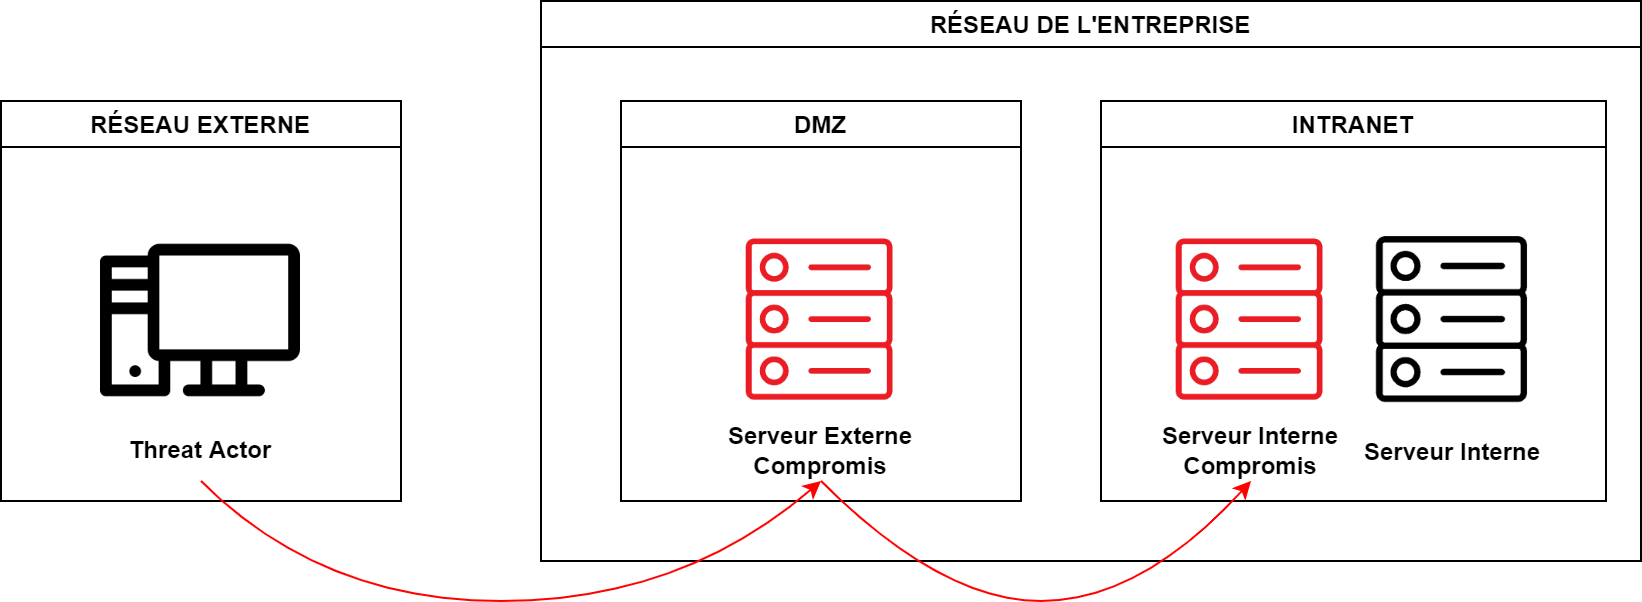
\includegraphics[width=0.95\linewidth]{images/attack-bridge/attack-bridge.png}
        }
    }
    \caption{Utilisation d'un serveur externe compromis comme pont pour entrer dans le réseau de l'entreprise.}
    \label{fig:attack-bridge}
\end{figure}

\begin{example}
    \hspace{0.45cm} Par exemple, dans le cas où un attaquant aurait compromis un serveur situé dans la DMZ (\textit{demilitarized zone}, zone démilitarisée en français) fournissant des services à la fois sur internet et sur le réseau interne de l'entreprise, il pourrait ensuite l'utiliser comme \textit{pont} pour rentrer dans le réseau interne de l'entreprise et y contaminer d'autres serveurs.

    Dans ce cas, les connexions réseaux de ce serveur compromis pourraient aider à déterminer quelles autres machines dans le réseau ont été compromises. Cette information se trouve presque toujours dans la RAM (et potentiellement dans le pare-feu ou dans les logs).
\end{example}

Sur la figure \ref{fig:device-physicalmemory}, on peut voir les objets NT gérés par l'Object Manager. Un driver avec des privilèges administrateurs peut accéder à la mémoire RAM directement via l'API WIN32 et ainsi la copier sur le disque. C'est ainsi que tous les outils de capture RAM fonctionnent.

% https://en.wikipedia.org/wiki/Object_Manager_(Windows)

\begin{figure}
    \centering
    \makebox[\textwidth]{
        \resizebox{18cm}{!}{
            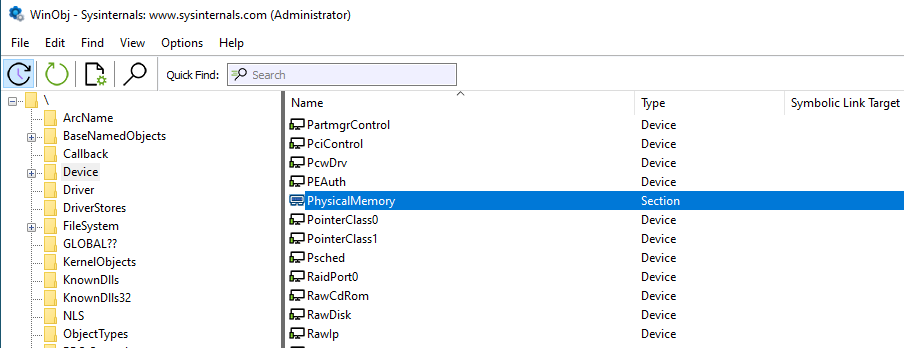
\includegraphics{images/RAM/WinObj-PhysicalMemory-Emplacement-RAM.png}
        }
    }
    \caption{Image de WinObj (de Sysinternals) montrant l'objet \textit{PhysicalMemory} auquel il faut accéder pour faire une image de la RAM.}
    \label{fig:device-physicalmemory}
\end{figure}



\subsection{Acquisition de la mémoire non-volatile}

Pour démarrer cette section, je vais tenter l'exercice de définir les données non-volatiles:

\begin{customquote}
    \hspace{0.45cm} Les données non-volatiles sont des données qui sont stockées sur la mémoire de masse. Elles ne sont donc pas perdues une fois que le système perd son alimentation électrique. Cependant, leur nature peut toujours être dynamique comme les logs qui peuvent être écrasés lorsque de nouveaux événements se produisent.
\end{customquote}

Contrairement à la mémoire RAM, la copie d'un disque peut également se faire lorsque le système est éteint. On peut même retirer le disque d'une machine éteinte pour le copier à l'aide d'un appareil forensique, ce qui évite totalement le risque d'écraser des données

Contrairement à la RAM, les données non-volatiles peuvent être extraites de la machine de plusieurs manières différentes. On peut, bien sûr, les copier avec un logiciel alors que le système est allumé. Par exemple, juste après avoir acquis une copie de la mémoire volatile. Mais elles peuvent aussi être copiées lorsque la machine est éteinte. On peut la redémarrer en bootant sur un autre système d'exploitation, situé sur une clé USB par exemple. Ou encore mieux, en retirant le disque dur de la machine pour le copier, de préférence en utilisant du matériel adapté à l'acquisition forensique. Toutes ces méthodes ne se valent pas d'un point de vue forensique, elles sont représentées sous la forme d'une pyramide sur la figure \ref{fig:non-volatile-memory} avec les méthodes préservant au mieux les données à la base et celles les préservant moins bien au sommet.

\begin{figure}
    \centering
    \makebox[\textwidth]{
        \resizebox{16cm}{!}{
            \includestandalone{images/pyramid-non-volatile-data/pyramid.tex}
        }
    }
    \caption{Pyramide des méthodes d'extraction des données non-volatiles.}
    \label{fig:non-volatile-memory}
\end{figure}

Parce que le stage a une durée limitée, j'ai décidé de me concentrer sur l'acquisition à chaud avec un disque externe, c'est-à-dire en branchant un disque dur externe lorsque le système est allumé et en utilisant un logiciel. L'avantage de cette méthode est qu'elle peut être utilisée juste après avoir effectué l'acquisition des données volatiles. Elle ne nécessite pas de connaître le mot de passe du BIOS ou de démonter l'ordinateur et elle est beaucoup plus rapide que lorsqu'on transfère les données via le réseau.






% LTeX: language=fr

\chapter{Solutions retenues}










\section{Acquisition forensique}

Il existe deux types de données forensiques: les données volatiles contenues dans la RAM et les données non-volatiles contenues sur le disque, chacune avec ses avantages et ses inconvénients.





\subsection{Données volatiles}

Pour acquérir les données de la RAM, il faut charger un logiciel dans la RAM, ce qui entraîne donc une modification de ces données. De plus, si un rootkit (logiciel malveillant persistant et furtif) est installé sur le système, il peut renvoyer des fausses informations, voir effacer ses traces en supprimant des données à la fois volatiles et non-volatiles comme des fichiers ou des clés de registres. Souvent, on considère que le jeu en vaut la chandelle et on prend ce risque. Cependant, cette décision doit être prise au préalable et pas sur le moment même. \cite{5}

Les outils que j'ai sélectionnés pour la capture de la RAM sont:

\begin{itemize}
    \item \textit{Belkasoft Live RAM Capturer} créé par Belkasoft;
    \item \textit{Magnet RAM Capture} créé par Magnet Forensics;
    \item \textit{FTK Imager} créé par Access Data.
\end{itemize}

\begin{figure}
    \centering
    \makebox[\textwidth]{
        \resizebox{19cm}{!}{
            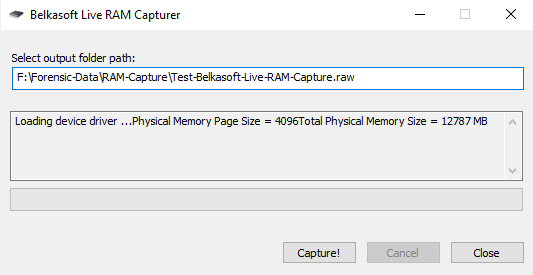
\includegraphics[width=14.45cm]{images/RAM/ram-capture-01.png}
            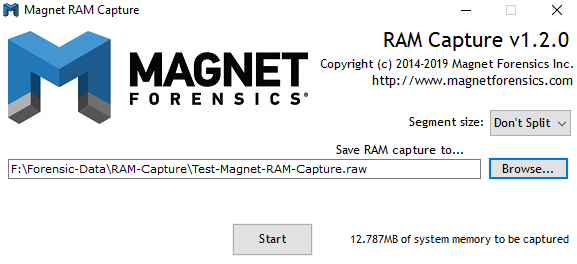
\includegraphics[width=14.45cm]{images/RAM/ram-capture-02.png}
        }
    }
    \caption{Interfaces graphiques des logiciels de capture RAM \textit{Belkasoft Live RAM Capturer} et \textit{Magnet RAM Capturer}.}
    \label{fig:ram-capture-softwares}
\end{figure}

La raison pour laquelle j'ai sélectionné ces trois logiciels est qu'ils ont été créés par des entreprises qui les supportent, mais aussi parce qu'ils sont gratuits. En fait, ces entreprises, fournissent des outils d'analyse forensique payants mais des logiciels d'acquisition de données forensiques gratuits. Ils ont donc tout intérêt à supporter ces logiciels, voir à les améliorer. D'abord, parce que c'est une porte d'entrée pour de nouveaux clients, mais aussi parce qu'en cas de problème, ils risqueraient de perdre des clients déjà acquis.

Parmi ces trois logiciels, Belkasoft Live RAM Capturer et Magnet RAM Capturer sont les plus simples d'utilisation car ils ont une interface extrêmement simple comme vous pouvez le voir sur la figure \ref{fig:ram-capture-softwares}. Mais pour les départager, j'ai aussi effectué des tests: des tests sur un PC de test et des tests sur une machine virtuelle dont j'ai fait une snapshot pour que les conditions soient les plus similaires possibles. Pour cela, j'ai fait la demande pour obtenir un PC de test chez NRB. J'ai ensuite testé l'acquisition de la mémoire vive avec ces logiciels et je les ai analysés avec le module \textit{windows.statistics.Statistics} du logiciel d'analyse \textit{volatility 3}, qui permet de comparer le nombre de pages mémoire invalides.

Le résultat est que \textit{Magnet RAM Capture} avec 141 345 pages invalides est moins bon que de \textit{Belkasoft Live RAM Capturer} avec seulement 46 629 pages invalides. Et ça se remarque d'ailleurs avec l'utilisation du module \textit{windows.pslist.PsList}, lequel montre un processus avec un PID extrêmement haut 104942906544106, et un nom de processus bizarre contenant des caractères unicodes: \texttt{<4{\quem}YJ{\quem\quem}wd{\quem}L!\quem}, ce qui montre une erreur de capture RAM. Ceci montre aussi l'importance d'effectuer une capture RAM avec le moins d'erreurs possible car on en retire de mauvaises informations.

Pour comprendre comment une page peut être est invalide, il faut comprendre le concept de \textit{mémoire virtuelle}. La mémoire virtuelle consiste à diviser la RAM en un certain nombre de pages ayant chacune une adresse. En traduisant les adresses virtuelles et les adresses réelles des pages RAM, le système d'exploitation simplifie l'utilisation de la RAM par les logiciels mais il peut aussi utiliser le mécanisme de swapping, c'est-à-dire utiliser l'espace disque comme extension de la RAM, ceci explique pourquoi la capture RAM est plus grande que la capacité du PC dont on fait l'image. \cite{7} Le module de statistique de Volatility 3 compte une page virtuelle comme invalide lorsque son adresse physique (la traduction de son adresse virtuelle) est invalide. \cite{8} Ça pourrait arriver, par exemple, si le contenu de la RAM change pendant la capture.

% https://thanursan.medium.com/comparison-of-memory-acquisition-software-for-windows-e8c6d981db23
% https://belkasoft.com/ram-capturer

\begin{table}
    \centering
    \begin{tabular}{cccc} \hline
            & \textbf{Belkasoft} & \textbf{Magnet} & \textbf{FTK Imager} \\ \hline
        \textbf{Temps d'acquisition}  & 90 secondes & 180 secondes & 90 secondes \\
        \textbf{VM - Pages invalides} & 60 010 & 2 180 438 & 2 174 110 \\
        \textbf{PC - Pages invalides} & 46 629 & 141 345 & 96 542 \\
        \textbf{RAM utilisée}         & 26.0 KB & 36.9 KB & 57.8 KB \\ \hline
    \end{tabular}
    \caption{Tableau de comparaison des outils de capture de mémoire RAM.}
    \label{tab:ram-capture}
\end{table}

En effectuant des tests et en prenant des mesures précises, j'ai pu arriver au tableau voir figure \ref{tab:ram-capture} qui permet de comparer de manière objective les différents outils et ainsi, de prendre une décision pour sélectionner quel outil devrait être utilisé lors des acquisitions de données volatiles. Mon choix s'est finalement porté sur l'outil de Belkasoft qui a été meilleur que les autres dans presque toutes les catégories. Pour mesurer la RAM utilisée, j'ai lancé les trois logiciels dans une VM dont j'avais pris une snapshot (un instantané) pour que les conditions soient les mêmes et j'ai utilisé Process Explorer pour mesurer la quantité de RAM utilisée comme vous pouvez le voir sur la figure \ref{fig:ram-used-magnet}.

\begin{figure}
    \centering
    \makebox[\textwidth]{
        \resizebox{18cm}{!}{
            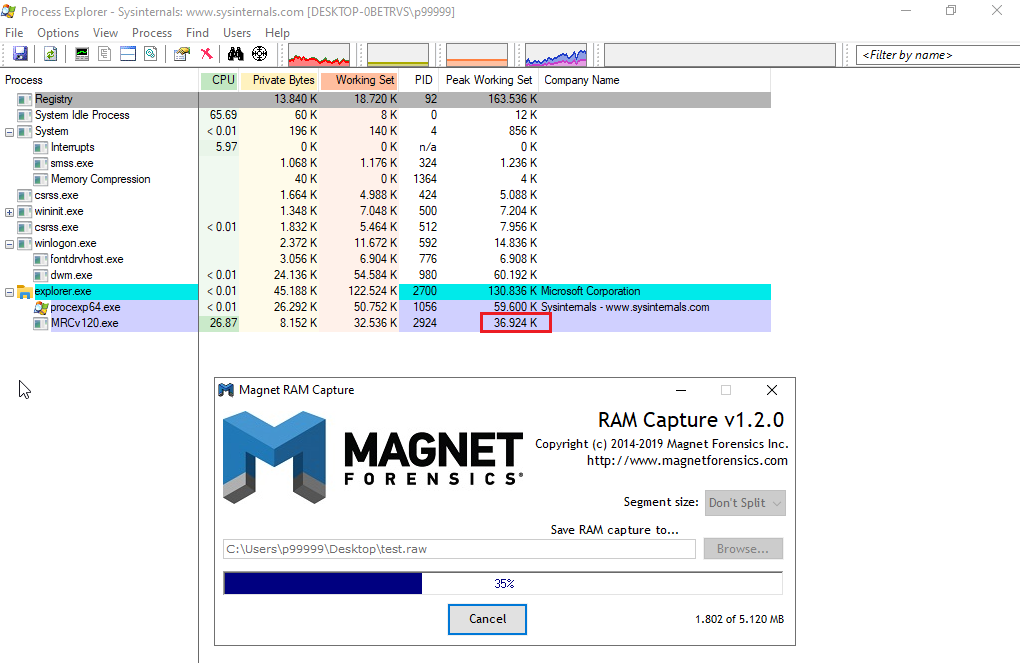
\includegraphics[width=14.45cm]{images/RAM/magnet-test-vm-02.png}
        }
    }
    \caption{Quantité de RAM utilisée par \textit{Magnet RAM Capturer} pendant la capture RAM, mesuré par \textit{Process Explorer} de Sysinternals.}
    \label{fig:ram-used-magnet}
\end{figure}





\subsection{Données non-volatiles}

J'ai sélectionné deux logiciels en utilisant la même réflexion que lors de la sélection de logiciels de capture de la mémoire volatile: que ce soient des logiciels qui sont proposés par des entreprises qui le tiennent à jour, et qu'ils soient gratuits. Les deux logiciels sont les suivants:

\begin{itemize}
    \item \textit{EnCase Forensic Imager} créé par EnCase;
    \item \textit{FTK Imager} créé par Access Data.
\end{itemize}

Malheureusement, je n'ai pas réussi à télécharger Encase Forensic Imager et ils n'ont pas répondu à ma prise de contact. Je n'ai donc pu qu'utiliser FTK Imager pour récupérer une image du disque d'un ordinateur.

\begin{figure}
    \centering
    \makebox[\textwidth]{
        \resizebox{19cm}{!}{
            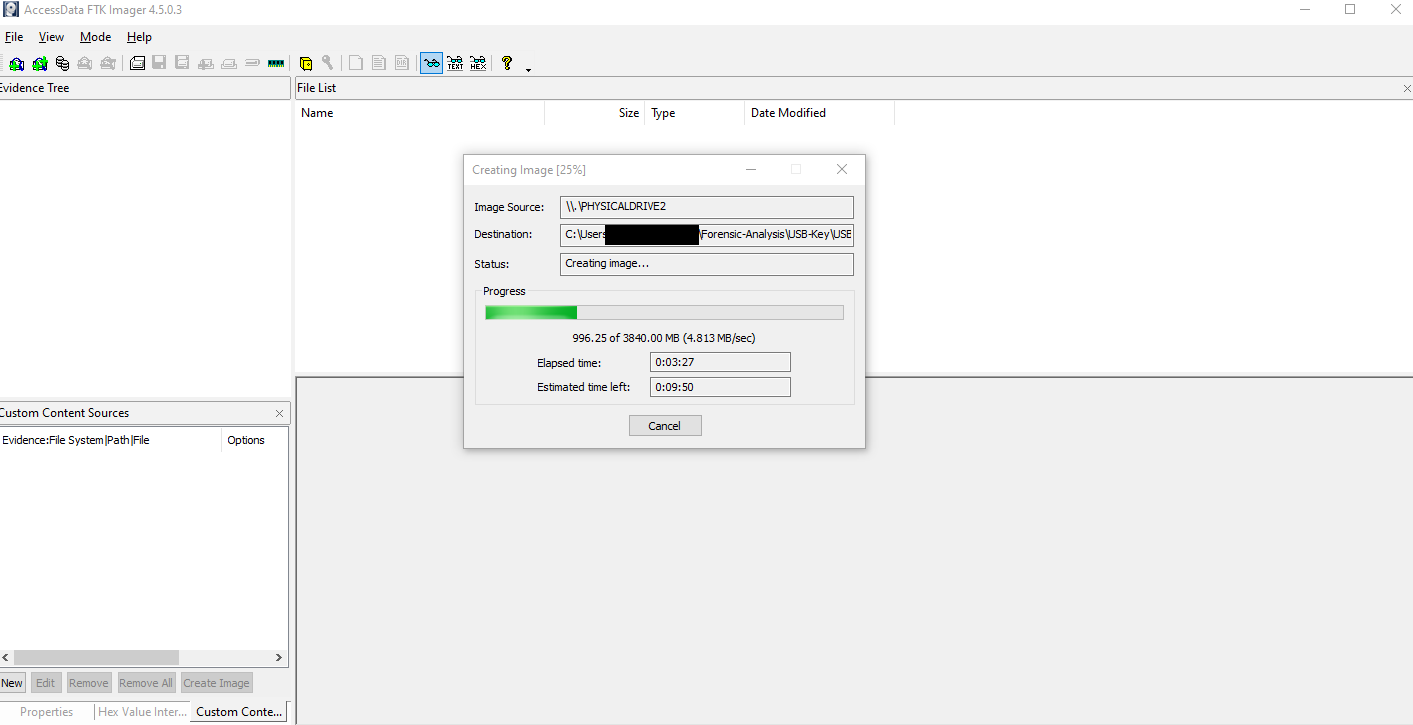
\includegraphics{images/Disque/FTK-Imager.png}
        }
    }
    \caption{Acquisition de la mémoire de masse avec FTK Imager.}
    \label{fig:ftk-imager}
\end{figure}

L'objectif n'est pas de récupérer que les fichiers utilisés par le système d'exploitation mais l'entièreté du disque. Y compris les espaces vides, qui peuvent contenir des données supprimées par un utilisateur ou un logiciel malveillant mais aussi les partitions qui ne sont pas utilisées par le système d'exploitation parce qu'elles pourraient également contenir des informations nécessaires à l'enquête.

Une des difficultés lorsqu'on copie l'entièreté d'un disque, est qu'on peut tomber sur un disque chiffré. Dans ce cas, il faut s'assurer de récupérer la clé de chiffrement. On peut le faire facilement pour les clés BitLocker avec la commande suivante (où il faut remplacer \texttt{<lettre-de-lecteur>} par la lettre représentant le disque dont on veut la clé, par exemple: C, pour le disque principal des PC Windows): \cite{11}

\texttt{manage-bde -protectors <lettre-de-lecteur> -get}










\section{Analyse forensique}





\subsection{Données volatiles}

Pour analyser ces données, il faut bien sûr utiliser des logiciels spécialisés. Il y a peu de logiciels qui permettent de le faire. J'en ai trouvé trois:

\begin{itemize}
    \item Volatility 2 et Volatility 3, un framework ainsi nommé parce qu'il sert à analyser les données volatiles. Volatility 2 est écrit en Python 2 et Volatility 3 en Python 3.
    \item Redline, un outil développé par l'entreprise FireEye.
\end{itemize}

Redline n'a plus été mis à jour depuis avril 2020. Bien qu'il supporte Windows Server 2019 et Windows 10, le logiciel a été incapable d'analyser la dernière version de ce système d'exploitation qui est utilisée dans l'entreprise lors des essais que j'ai réalisés.

Pour ce qui est du framework Volatility, la version 2 n'est plus supportée, tout comme le langage dans lequel elle a été écrite, Python 2. Cependant, Volatility 2 a encore beaucoup de plugins écrits par la communauté qui n'ont pas été réécrits pour fonctionner avec la dernière version. À l'avenir, il faudra bien passer à l'utilisation de Volatility 3, par exemple pour analyser des machines Windows 11 mais en attendant, j'ai décidé de continuer à travailler avec Volatility 2.

\begin{example}
    \hspace{0.45cm} Le \textit{process hollowing} est une sous-technique de l'injection de code malicieux, référencé par l'ID T1055.012 par l'organisation MITRE. Elle est réalisée par des malwares pour éviter d'être détectés par l'anti-virus de la machine. Un processus créé un nouveau processus enfant inoffensif dans un état suspendu, ensuite, il y injecte du code malicieux. \cite{10}

    Le plugin \textit{HollowFind} a été écrit par un chercheur en cybersécurité pour Volatility 2. Il sert à trouver les processus dans lesquels on a injecté du code malicieux avec la méthode de process hollowing. Ce n'est qu'un exemple parmi d'autres de plugins écrits par la communauté qui manquent à la dernière version de Volatility.
\end{example}





\subsection{Données non-volatiles}


\begin{figure}
    \centering
    \makebox[\textwidth]{
        \resizebox{16cm}{!}{
            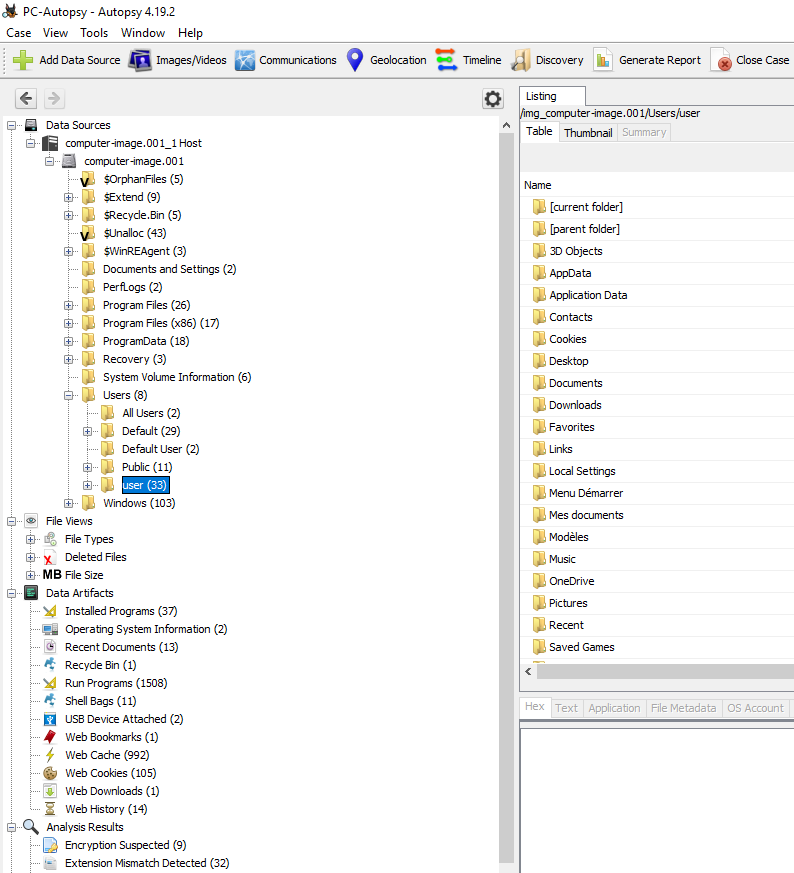
\includegraphics{images/Disque/autopsy-11.png}
        }
    }
    \caption{Autopsy, logiciel d'analyse de mémoire de masse.}
    \label{fig:autopsy-overview}
\end{figure}

Pour analyser les données non-volatiles, il existe plusieurs logiciels gratuits de grande qualité et qui se complètent:

\begin{enumerate}
    \item Autopsy est un logiciel open source qui fonctionne avec une série de modules. Il scanne l'image disque pour lister les volumes et l'arborescence du système de fichier. Il cherche aussi les fichiers supprimés et catégorise les fichiers en fonction de leur taille et de leur extension. Ensuite, on peut choisir de lancer des modules comme l'extracteur d'archives, le détecteur de mauvaise extension, l'analyseur d'emails, etc. Un des plus utiles est le module d'activité récente qui sert à récupérer la liste des documents récents, les données des navigateurs WEB, ainsi que la liste des programmes installés. Autopsy prend beaucoup de temps pour effectuer ces analyses en raison des grandes quantités de données contenues sur un disque. Vous pouvez le voir sur la figure \ref{fig:autopsy-overview}.
    \item Kape et les outils d'Éric Zimmerman fonctionnent de concert pour récupérer des artefacts forensiques de grande importance d'une machine et les analyser. Par exemple, on peut utiliser Kape pour récupérer la MFT (la \textit{master file table}, index principal du système de fichier NTFS) et en normaliser les données pour ensuite les analyser avec l'outil \textit{Timeline Explorer} d'Éric Zimmerman. On peut aussi utiliser Kape pour récupérer les registres et les logs de registres afin de les nettoyer puis les analyser avec l'outil \textit{Registry Explorer} de Zimmerman.
    \item Splunk est un outil SIEM (\textit{Security Information and Event Management}) qui sert à analyser les logs. Un log est l'enregistrement d'un évènement qui s'est produit sur un système informatique, par exemple: lorsqu'une clé USB a été branchée ou débranchée. Cet outil est déjà en place dans l'entreprise.
    \item Chainsaw est un outil d'analyse de logs Windows open source créé par l'entreprise F-Secure (figure \ref{fig:chainsaw}). Il utilise un ensemble de règles pour déterminer si des événements pertinents du point de vue de la cybersécurité se sont produits comme du mouvement latéral, c'est-à-dire le déplacement d'un attaquant au sein du réseau de l'entreprise.
    \item Thor Lite est un scanner anti-virus gratuit qui a bien sûr des limitations par rapport à la version payante parce qu'avec la version Lite, on peut scanner les exécutables mais pas certains types de fichiers comme les raccourcis Windows (d'extension \textit{.lnk}). Dans sa version payante, il va également aller scanner les clés de registres et autres endroits où les malwares peuvent aller se cacher. C'est cependant un outil déjà très utile dans sa version Lite puisqu'il nous sert à repasser là où d'autres anti-virus, comme Windows Defender, ont échoué.
\end{enumerate}

\begin{figure}
    \centering
    \makebox[\textwidth]{
        \resizebox{19cm}{!}{
            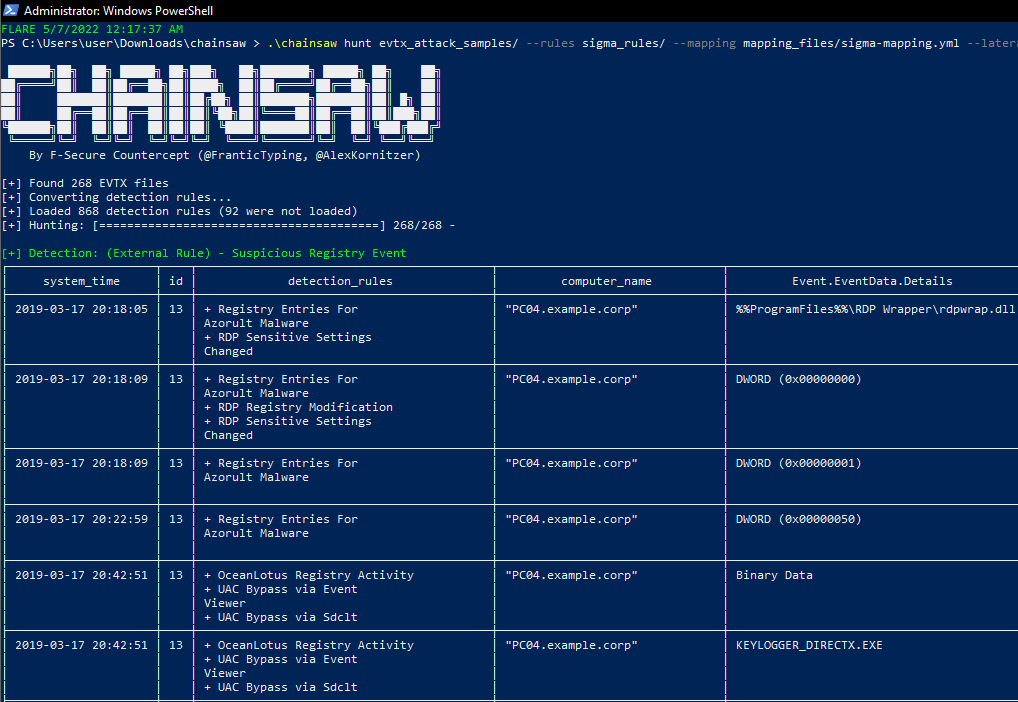
\includegraphics{images/Disque/chainsaw-03.png}
        }
    }
    \caption{Utilisation de chainsaw sur des logs Windows de test.}
    \label{fig:chainsaw}
\end{figure}

Les logiciels se complètent parce qu'on peut les utiliser pour naviguer dans le système de fichiers, analyser les fichiers supprimés, les dossiers consultés, mais aussi trouver les logiciels malveillants dans le système de fichiers, essayer de comprendre ce que l'acteur malveillant a fait sur le système, etc. Aucun d'entre eux ne peut tout faire seul mais en les combinant, on arrive à récupérer un maximum d'informations pour nous aider à comprendre et résoudre l'incident.

Malheureusement, ces outils ne peuvent pas tous analyser l'image disque directement. Certains le peuvent, comme Autopsy, mais dans le cas où le disque de la machine à analyser a été chiffré, les informations récupérées seront très pauvres. On pourrait récupérer la liste des partitions mais aucune information venant du système de fichiers parce que ces informations sont illisibles. Dans ce cas, il faut utiliser l'outil \textit{Arsenal Image Mounter} qui est un logiciel gratuit (avec une version payante) permettant de monter l'image disque comme si on venait de brancher une clé USB. Le logiciel permet de monter l'image en read-only (figure \ref{fig:arsenal-image-mounter}). Une fois montée, on peut facilement sélectionner le disque dans l'explorateur de fichiers pour le déchiffrer avec la clé BitLocker (figure \ref{fig:bitlocker}).

\begin{figure}
    \centering
    \makebox[\textwidth]{
        \resizebox{18cm}{!}{
            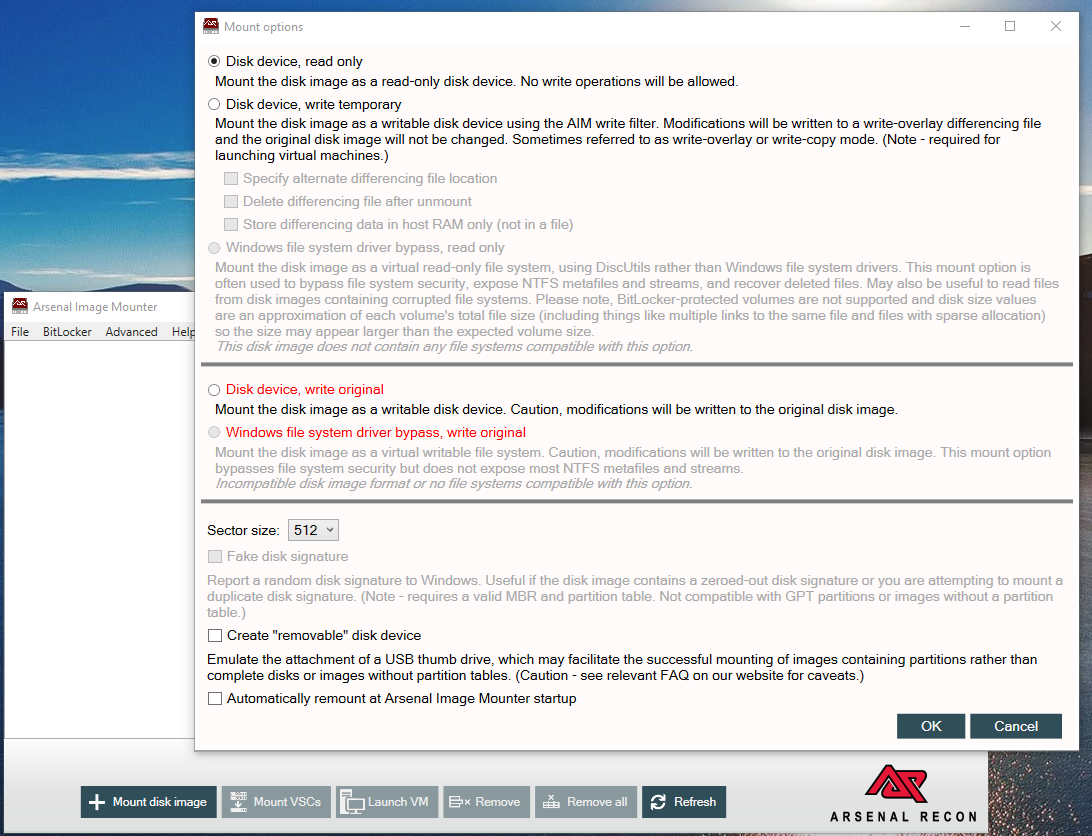
\includegraphics{images/Disque/arsenal-image-mounter-01.png}
        }
    }
    \caption{Montage d'une image disque en lecture seule avec Arsenal Image Mounter.}
    \label{fig:arsenal-image-mounter}
\end{figure}

\begin{figure}
    \centering
    \makebox[\textwidth]{
        \resizebox{10cm}{!}{
            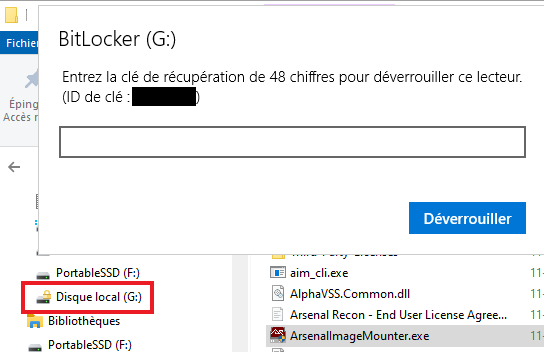
\includegraphics{images/Disque/arsenal-image-mounter-04.png}
        }
    }
    \caption{Déchiffrement d'une image disque montée chiffrée avec BitLocker.}
    \label{fig:bitlocker}
\end{figure}





\subsection{Données externes}

L'analyse forensique ne se contente généralement pas à une seule machine mais elle s'étend également à un ensemble d'appareils qui font partie du système informatique. Par exemple, c'est aussi très important d'exporter les données provenant des pare-feux, des proxys, des solutions de monitoring ou de management d'endpoints comme Microsoft EDR. En particulier si les informations provenant de ces appareils ne sont conservés que sur de courtes périodes. Leur analyse, généralement à l'aide d'un outil de SIEM comme Splunk peut changer le cours d'une enquête forensique ou tout du moins apporter beaucoup d'informations.

\begin{example}
    \hspace{0.45cm} Dans le cas où la machine d'un développeur a été compromise, il est naturel de suspecter qu'il y a pu y avoir du mouvement latéral, c'est-à-dire, que l'attaquant s'est déplacé dans le réseau en compromettant d'autres postes de travail ou des serveurs auxquels la victime a accès. En analysant les logs du pare-feu et des serveurs, si on ne trouve aucune connexion pendant la période d'infection, ça peut indiquer que la contamination est restée localisée.

    De plus, si l'attaquant a été furtif, il a potentiellement effacé les traces de son passage sur le système au fur et à mesure qu'il effectuait des actions. Dans ce cas, c'est particulièrement important de récupérer les logs des autres appareils ou d'aller les recherches dans l'outil de monitoring comme Microsoft EDR ou Splunk.
\end{example}










\section{Solution de sandbox}

Sandbox veut dire \textit{bac à sable} en anglais. Ce terme est utilisé en informatique pour désigner un environnement isolé dans lequel on peut faire tourner un logiciel sans qu'il y ait de conséquences négatives sur le reste de l'ordinateur. Grâce à ces sandboxes, un utilisateur peut exécuter un programme potentiellement dangereux sans mettre en danger ses données, ni endommager son système. Par abus de langage, on appelle aussi \textit{sandbox}, un logiciel qui analyse automatiquement le comportement des logiciels et documents malveillants dans un environnement isolé. Ce logiciel reçoit en entrée un fichier et le place dans une sandbox pour le \textit{détonner}. En sortie, ce logiciel donnera un rapport dans lequel le comportement du fichier est analysé. Ces sandboxes contiennent un système d'exploitation, souvent \textit{Windows}, et des logiciels régulièrement exploités par des acteurs malveillants comme Adobe Acrobat, Microsoft Excel ou Microsoft Word. Les logiciels malveillants que nous cherchons à analyser sont appelés \textit{malwares} pour \textit{malicious software} et \textit{maldoc}, abréviation de \textit{malicious document}, lorsqu'ils sont inclus dans un document PDF, Word ou autre.

Comme expliqué, certains produits appelés sandbox ne correspondent pas à ce que nous cherchons, parmi ceux-ci, il y a: Microsoft Sandbox, Sandboxie, Shade Sandbox, etc. Parmi les autres critères de comparaison que nous allons utiliser, il y a:
\begin{itemize}
    \item Le \textit{prix}, si certaines sandboxes sont gratuites et open source, les solutions commerciales peuvent coûter de quelques centaines d'euros à plusieurs dizaines de milliers d'euros par an.
    \item S'il existe une \textit{version communauté gratuite}, en général, c'est une version restreinte et pour obtenir toutes les fonctionnalités, il faut passer à la version payante.
    \item Si c'est une \textit{solution indépendante} ou si elle fait partie d'une solution d'EDR (Endpoint Detection and Response) ou d'une suite antivirus.
    \item Les \textit{plateformes supportées}, c'est-à-dire si on peut analyser des malwares qui ne tournent que sur Windows, ou si on peut également analyser des malwares qui tournent sur Linux, macOS ou Android.
    \item Le \textit{service proposé}, est-ce qu'on y a accès uniquement via un SaaS (Software as a Service) ? Est-ce une solution hardware ou une VM qu'on peut installer sur un hyperviseur ou dans le cloud ?
    \item Peut-on \textit{interagir manuellement} avec l'analyse ? Certains malwares requièrent une interaction humaine pour s'activer.
    \item Est-ce possible d'exporter les données forensiques de la sandbox, comme une capture de la RAM ou un enregistrement des paquets échangés sur le réseau pour une analyse forensique manuelle plus poussée ?
\end{itemize}

En fin de compte, j'ai décidé de diviser les solutions en trois catégories en fonction du prix:
\begin{enumerate}
    \item Les sandboxes gratuites (table \ref{tab:sandbox-gratuites}).
    \item Les sandboxes qui ont une version communauté gratuite (table \ref{tab:sandbox-community}).
    \item Les sandboxes qui ne possèdent qu'une version payante (table \ref{tab:sandbox-payantes}).
\end{enumerate}

Finalement, nous avons choisi de garder la sandbox \textit{CAPEv2} pour plusieurs raisons:
\begin{enumerate}
    \item Parce que c'est une solution open source gratuite.
    \item Parce qu'on peut la faire tourner \textit{on premise}, c'est-à-dire sur l'infrastructure NRB pour éviter que des informations sensibles ne puissent fuiter.
    \item Parce qu'elle supporte à la fois Windows et Linux qui sont les deux systèmes utilisés dans l'entreprise.
    \item Parce qu'elle contient beaucoup de fonctionnalités avancées comme un débogueur intégré, ce qui permet de contrôler le flux d'exécution d'un malware qui tenterait d'échapper à l'analyse automatique.
    \item Parce que c'est un projet qui est maintenu par une communauté de développeurs active.
\end{enumerate}

Sur le tableau de comparaison \ref{tab:sandbox-gratuites}, la sandbox \textit{Cuckoo} semble posséder plus de caractéristiques positives que \textit{CAPEv2}, alors pourquoi ne pas la prendre ? Le problème des solutions open source est qu'il faut qu'elles trouvent des développeurs motivés pour rester à jour, ce qui ne semble pas être le cas de Cuckoo. Par exemple, cette sandbox est toujours codée dans le langage de programmation python 2 qui n'est lui-même plus supporté par des développeurs. Ce manque de soutien de la part de la communauté peut entraîner des risques de sécurité si on trouve des vulnérabilités dans la sandbox, ils risquent de ne pas être corrigés.

En choisissant CAPEv2, qui est un \textit{fork} (une copie du code en quelque sorte) de Cuckoo et donc possède la même architecture logicielle et la même API (\textit{application programming interface} en anglais), j'ai choisi une sorte de "Cuckoo amélioré" parce que les développeurs en ont modifié le code pour le passer sous python 3 (la version actuelle de python) et y ont ajouté des fonctionnalités. Cependant, ils ont arrêté de faire des tests pour supporter des sandboxes Android.

La sandbox Cuckoo3 est également un fork de Cuckoo qui a simplement fait passer le logiciel sous python 3 mais sans ajouter de nouvelles fonctionnalités, il en a même perdu comme le support du système d'exploitation Android. Il a malgré cela l'avantage d'être soutenu par le CERT de l'Estonie (CERT est l'acronyme de Computer Emergency Response Team). DRAKVUF Sandbox est une sandbox créée par un autre CERT, celui de la Pologne. Son grand avantage est qu'il ne fait pas tourner d'agent sur la machine virtuelle imbriquée mais qu'il va monitorer le comportement du malware depuis l'extérieur via l'hyperviseur, ce qui le rend beaucoup plus difficile à détecter par le malware. En revanche, ses fonctionnalités sont moins complètes que d'autres Sandbox comme CAPE.

\newpage

\begin{tikzpicture}[remember picture, overlay]
    \node () [text width=20cm] at ($(current page.center)+(0,8.5)$) {
        \begin{table}[H]
            \centering
            \begin{tabular}{cccccc} \hline
                    & \textbf{Cuckoo} & \textbf{CAPEv2} & \textbf{Limon} & \textbf{Cuckoo3} & \textbf{Drackvuf} \\ \hline
                \textbf{Solution indépendante} & \oui & \oui & \oui & \oui & \oui \\ \hline
                \textbf{SaaS}       & \oui & \oui & \non & \non & \non \\
                \textbf{Cloud}      & \oui & \oui & \oui & \oui & \oui \\
                \textbf{Hardware}   & \non & \non & \non & \non & \non \\ \hline
                \textbf{Windows}    & \oui & \oui & \non & \oui & \oui \\
                \textbf{Linux}      & \oui & \oui & \oui & \oui & \non \\
                \textbf{Android}    & \oui & \non & \non & \non & \non \\
                \textbf{macOS}      & \oui & \oui & \non & \non & \non \\ \hline
                \textbf{Interaction manuelle} & \oui & \oui & \non & \oui & \oui \\
                \textbf{Export de données forensiques} & \oui & \oui & \oui & \oui & \oui \\ \hline
            \end{tabular}
            \caption{Tableau de comparaison des sandboxes gratuites.}
            \label{tab:sandbox-gratuites}
        \end{table}
    };
    \node () [text width=20cm] at ($(current page.center)+(0,1.5)$) {
        \begin{table}[H]
            \centering
            \begin{tabular}{ccccc} \hline
                    & \textbf{Joe Sandbox} & \textbf{Falcon} & \textbf{any.run} & \textbf{Metadefender} \\ \hline
                \textbf{Solution indépendante} & \oui & \oui & \oui & \oui \\ \hline
                \textbf{SaaS}       & \oui & \oui & \oui & \oui \\
                \textbf{Cloud}      & \oui & \non & \non & \non \\
                \textbf{Hardware}   & \non & \non & \non & \non \\ \hline
                \textbf{Windows}    & \oui & \oui & \oui & \oui \\
                \textbf{Linux}      & \oui & \oui & \non & \non \\
                \textbf{Android}    & \oui & \oui & \non & \non \\
                \textbf{macOS}      & \oui & \oui & \non & \non \\ \hline
                \textbf{Interaction manuelle} & \non & \non & \oui & \non \\
                \textbf{Export de données forensiques} & \oui & \oui & \oui & \non \\ \hline
            \end{tabular}
            \caption{Tableau de comparaison des sandboxes avec une version communauté gratuite.}
            \label{tab:sandbox-community}
        \end{table}
    };
    \node () [text width=20cm] at ($(current page.center)+(0,-6.50)$) {
        \begin{table}[H]
            \centering
            \begin{tabular}{ccccccc} \hline
                    & \rothead{\textbf{Symantec}} & \rothead{\textbf{Kaspersky}} & \rothead{\textbf{McAfee}} & \rothead{\textbf{Fireye}} & \rothead{\textbf{Trend Micro}} & \rothead{\textbf{Cisco TG}} \\ \hline
                \textbf{Solution indépendante} & \non & \non & \non & \non & \oui & \oui \\ \hline
                \textbf{SaaS}       & \oui & \non & \non & \non & \non & \non \\
                \textbf{Cloud}      & \oui & \non & \oui & \non & \oui & \oui \\
                \textbf{Hardware}   & \oui & \oui & \oui & \oui & \oui & \oui \\ \hline
                \textbf{Windows}    & \oui & \oui & \oui & \oui & \oui & \oui \\
                \textbf{Linux}      & \non & \non & \non & \non & \non & \non \\
                \textbf{Android}    & \oui & \oui & \oui & \non & \oui & \non \\
                \textbf{macOS}      & \non & \non & \non & \oui & \oui & \non \\ \hline
                \textbf{Interaction manuelle} & \non & \non & \oui & \oui & \non & \oui \\
                \textbf{Export de données forensiques} & \non & \oui & \oui & \non & \non & \oui \\ \hline
            \end{tabular}
            \caption{Tableau de comparaison des sandboxes payantes.}
            \label{tab:sandbox-payantes}
        \end{table}
    };
\end{tikzpicture}

\newpage

L'installation de CAPE est une tâche ardue mais son utilisation est plus aisée. Elle se fait via une interface web (figure \ref{fig:cape-01}) sur laquelle il suffit de cliquer sur le bouton \textit{Submit} puis de choisir le fichier qui sera ensuite testé automatiquement dans la machine virtuelle Windows qui sera recréée pour chaque échantillon soumis à partir d'une snapshot. Une snapshot étant un instantané de la machine à un moment T pour éviter que les conditions soient toujours les mêmes peu importe l'ordre de soumissions. En effet, si on soumet un rootkit deux fois dans une machine qui n'a pas été restaurée, la première fois, il sera détecté comme malicieux mais la seconde, il restera indétecté parce que la première installation cachera le comportement malicieux du second.

Une fois l'analyse effectuée, on peut en voir les résultats avec un résumé coloré comme sur la figure \ref{fig:cape-01} où les trouvailles les plus importantes sont exposées avec des couleurs indiquant leur dangerosité potentielle. On peut aussi voir le détail des fichiers ou des clés de registres ouverts et modifiés. Ou encore récupérer le dump des processus malicieux ou le dump réseau (fichier pcap contenant tous les paquets réseau) pour analyse avec wireshark par exemple.

\begin{figure}
    \centering
    \makebox[\textwidth]{
        \resizebox{18cm}{!}{
            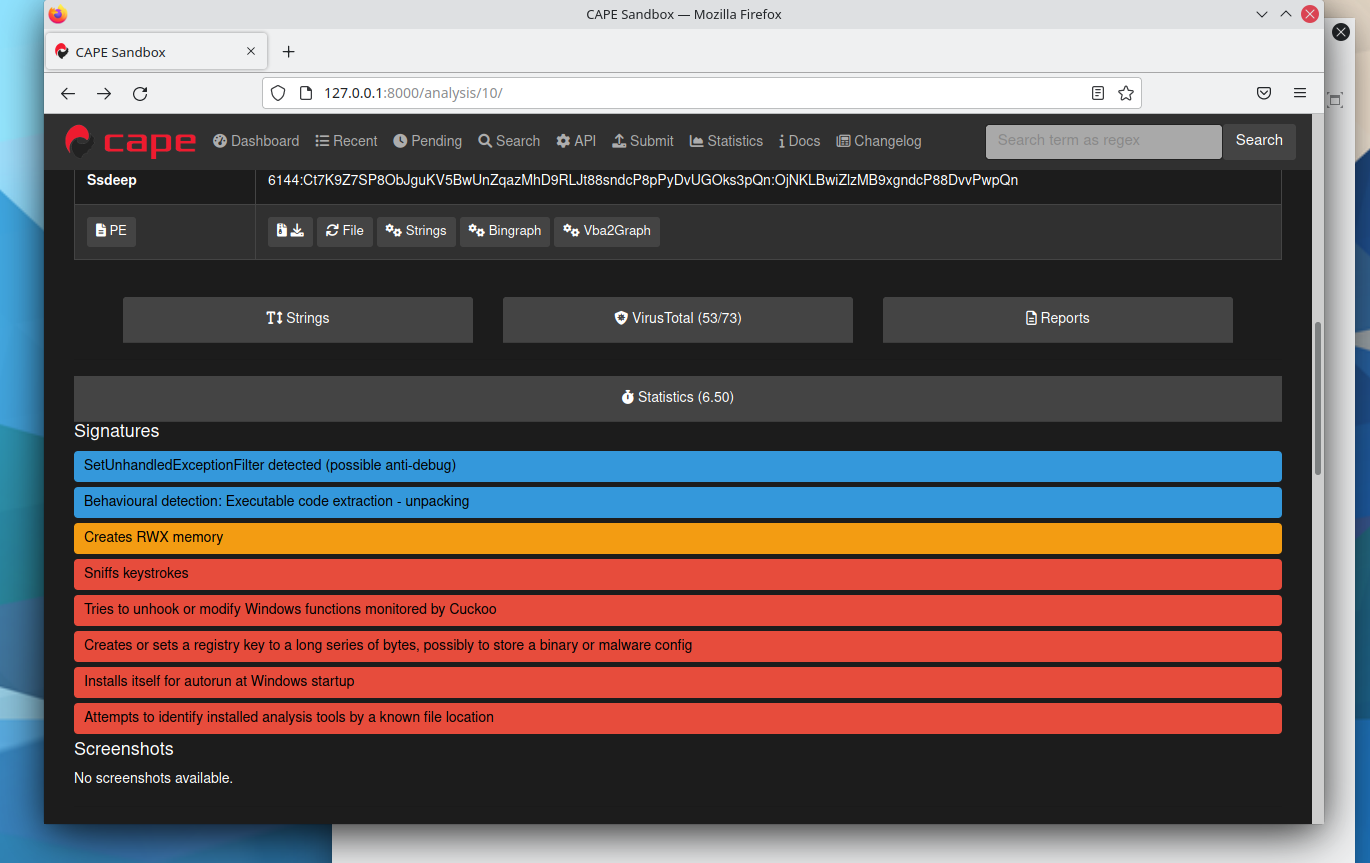
\includegraphics{images/malware/cape-sandbox-exemple.png}
        }
    }
    \caption{Résultats de l'analyse dynamique automatique d'un exécutable avec CAPE Sandbox.}
    \label{fig:cape-01}
\end{figure}

Malheureusement, la machine virtuelle imbriquée lancée par CAPE Sandbox plante complètement (voir figure \ref{fig:sandbox-fail}) lorsqu'on essaie d'analyser un document Office, ce qui n'est pas le cas lorsqu'on essaie d'analyser d'autres types de documents comme des exécutables ou des fichiers PDF. Après plusieurs jours de travail pour essayer de corriger le problème avec Excel, j'ai essayé de passer sur Libre Office. Bien que ça évite le fait que la sandbox affiche un écran bleu, l'analyse ne s'effectuait pas correctement. À nouveau, après plusieurs jours, j'ai dû mettre de côté ce problème pour continuer sur le reste du travail.

\begin{figure}
    \centering
    \makebox[\textwidth]{
        \resizebox{15cm}{!}{
            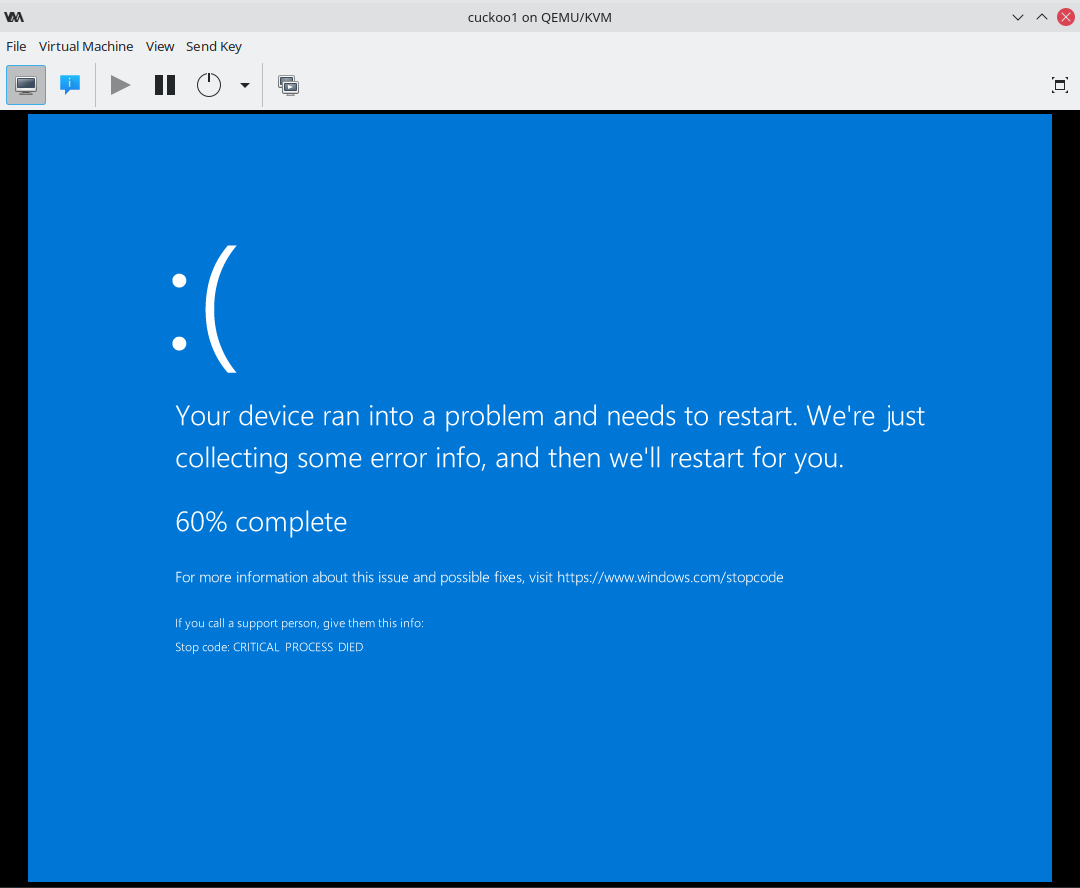
\includegraphics{images/malware/excel-blue-screen-of-death.png}
        }
    }
    \caption{La VM imbriquée plante lorsqu'on essaie d'analyser un document Office.}
    \label{fig:sandbox-fail}
\end{figure}










\section{Analyse de malwares}

Pour analyser les logiciels et documents malveillants, plus communément appelés malwares, j'ai commencé en listant une série d'outils. J'y ai mis des outils d'analyse de documents PDF, d'autres pour analyser les documents Office XML (ceux qui ont une extension terminant par x comme .docx ou .xlsx), les documents Office binaire (les anciens formats avec les extensions .doc, .xls, etc.), les exécutables PE, et encore d'autres. Mais ça rend l'analyse un malware complexe parce qu'il faut maîtriser un grand nombre d'outils pour réussir à analyser tous les types possibles. La solution est d'utiliser la plateforme automatisée \textit{FAME} dévelopée par le CERT (Computer Emergency Response Team) de la Société Générale. C'est l'acronyme de \textit{FAME Automates Malware Evaluation}.

\begin{figure}
    \centering
    \makebox[\textwidth]{
        \resizebox{18cm}{!}{
            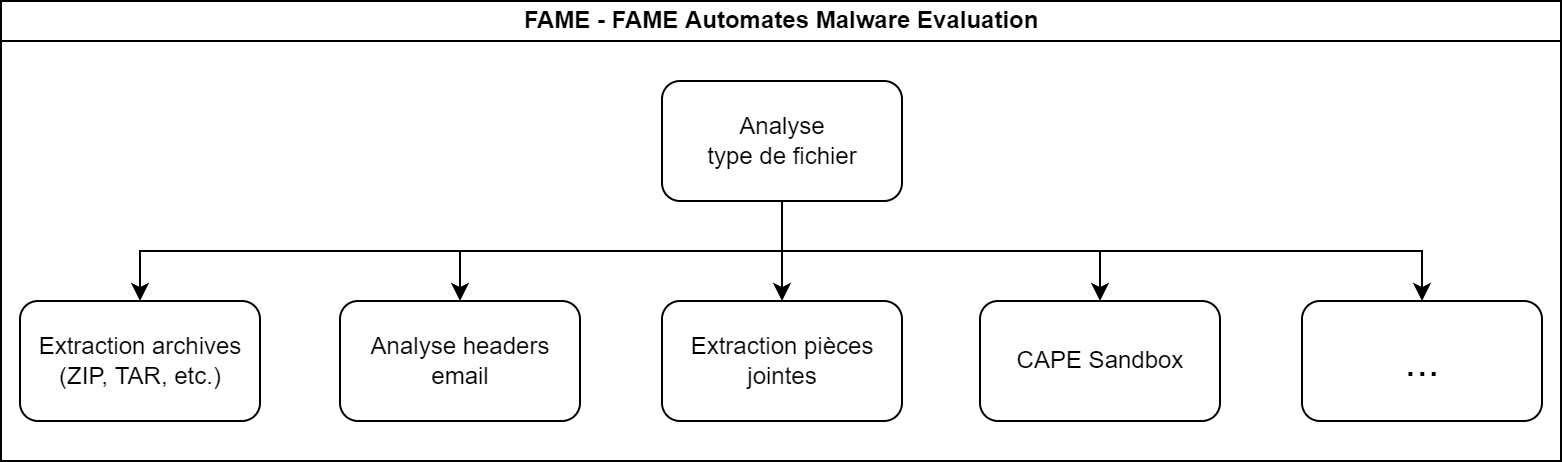
\includegraphics{images/fame-malware-analysis/fame.png}
        }
    }
    \caption{Schéma montrant le fonctionnement de FAME.}
    \label{fig:fame-explanation}
\end{figure}

Comme le montre le schéma sur la figure \ref{fig:fame-explanation}, quand on soumet un fichier à la plateforme, elle commence par déterminer son type afin de décider quels modules vont être lancés. Par exemple, dans le cas d'un document Excel, FAME va lancer à la fois un module d'analyse des métadonnées, un module d'analyse des macros Office, un module d'aperçu qui va générer des images montrant le contenu du document, ainsi que la sandbox pour effectuer une analyse dynamique en simulant l'ouverture du document Excel comme un utilisateur réel le ferait pour voir les actions que les macros vont effectuer sur le système.

Comme vous l'aurez compris, FAME fonctionne avec une série de modules dont un module qui interagit avec la sandbox pour soumettre le fichier malicieux et récupérer les résultats. Il n'y a pas de module fonctionnant avec CAPE, la sandbox choisie et installée dans l'infrastructure d'analyse. Cependant, il y a des modules adaptés à la sandbox Cuckoo dont CAPE est un fork. Ça veut dire qu'on peut facilement adapter le code d'un de ces modules pour le faire fonctionner avec la sandbox déjà installée.

L'utilisation de cette plateforme apporte deux grands avantages:
\begin{itemize}
    \item Elle permet de gagner du temps lorsqu'il y a beaucoup de petites analyses à effectuer. Par exemple, s'il y a une dizaine de cas de phishing à analyser avec parfois plusieurs pièces jointes par email, l'utilisation de FAME permet de gagner du temps en automatisant l'analyse. En fait, en temps normal, un analyste n'aurait peut-être pas le temps d'effectuer toutes les analyses et les domaines malveillants utilisés par les adversaires ne seraient probablement pas bloqués. En libérant du temps, l'analyse peut-être plus poussée et ça renforce la sécurité de l'entreprise.
    \item Cette plateforme peut aussi servir dans les investigations forensiques plus poussées où on a réussi à identifier le malware. Grâce à cette plateforme, on peut ainsi obtenir une première analyse ou effectuer un premier tri s'il y a beaucoup de fichiers à analyser. Il faudra malgré tout effectuer une analyse manuelle si c'est nécessaire pour le bon avancement de l'enquête.
\end{itemize}

\begin{figure}
    \centering
    \makebox[\textwidth]{
        \resizebox{16cm}{!}{
            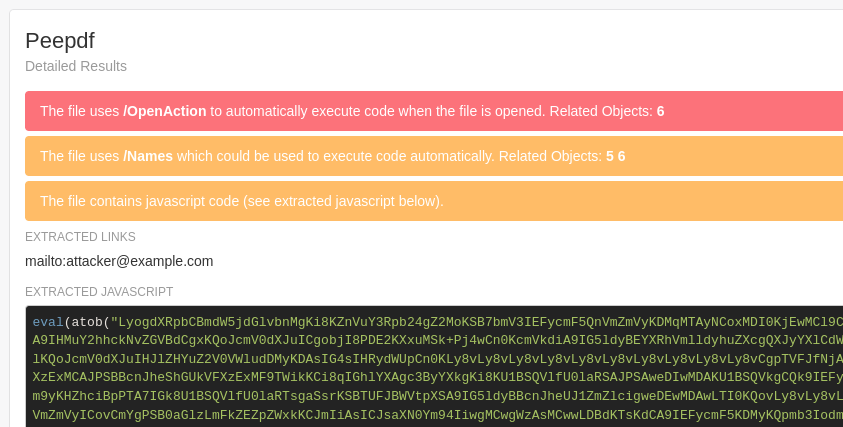
\includegraphics{images/malware/fame-pdf.png}
        }
    }
    \caption{Analyse d'un fichier PDF par FAME qui en extrait les liens, le javascript et émet des alertes.}
    \label{fig:fame-pdf-analysis}
\end{figure}

\begin{example}
    \hspace{0.45cm} Par exemple, si un employé du département des ressources humaines reçoit un PDF vérolé par email, il se peut qu'il remarque une activité suspecte et le signale, ou bien que l'outil de monitoring de sa machine (comme \textit{Microsoft Endpoint Detection and Response}) le détecte. À partir de là, un analyste peut demander à récupérer le PDF ou l'email. En le soumettant dans FAME, on va avoir un résultat comme sur la figure \ref{fig:fame-pdf-analysis} qui montre bien que le document est malicieux. En analysant le code manuellement, on pourrait retrouver des indicateurs de compromissions comme des adresses IP ou des noms de domaines qu'on pourrait ensuite ajouter sur une blacklist pour éviter d'être compromis à l'avenir. Ces indicateurs servent aussi à chercher si d'autres machines n'ont pas déjà été compromises en regardant dans l'outil de SIEM (comme \textit{Splunk}) pour vérifier si d'autres machines les ont déjà contactés.
\end{example}










\section{Distributions de forensique}

Une distribution est un ensemble de logiciels groupés ensemble, ça vient de l'anglais \textit{software distribution}. Et donc une distribution orientée forensique est une collection de logiciels utilisés dans le processus forensique. Ce terme s'applique plus généralement au système d'exploitation Linux mais dans notre cas, il y a aussi des distributions Windows qui sont donc des ensembles d'outils regroupés ensemble qui ne fonctionnent que sur le système d'exploitation Windows.

Un des avantages d'utiliser une distribution toute faite est qu'elle contient des outils dont on ne sait pas encore qu'on en a besoin. Par exemple, admettons qu'on tombe sur un malware écrit dans le langage de programmation python, certains outils pour l'analyser seront déjà présents sur nos machines d'analyse. C'est un énorme avantage surtout que l'infrastructure d'analyse est isolée d'internet et l'installation d'un outil supplémentaire est donc plus ardue, en plus de prendre beaucoup de temps.

Bien entendu, ce n'est pas impossible d'ajouter des logiciels supplémentaires qui ne sont pas compris dans les distributions. C'est d'ailleurs ce que j'ai fait en ajoutant des logiciels gratuits mais avec une licence les empêchant d'être inclus par défaut (par exemple: \textit{Kape} requiert l'inscription d'un utilisateur sur le site de \textit{Kroll}, l'entreprise qui crée le logiciel pour pouvoir le télécharger).

Parce que certains outils n'existent que sur Windows et d'autres que sur Linux, un des besoins principal dans le choix de la distribution est d'avoir deux machines. L'autre besoin est qu'il y ait une grande variété de logiciels pour que les machines virtuelles créées puissent être utilisés dans des situations diverses et variées.

Voici une liste des distributions Linux orientées analyse forensique intéressantes:

\begin{itemize}
    \item \textit{SOF-ELK}, abréviation de Security Operations and Forensics - ElasticSearch LogStash Kibana. Elle est basée sur Ubuntu et se concentre sur l'analyse de logs avec le SIEM ELK préinstallé et déjà configuré pour cela.
    \item \textit{SIFT Workstation}, abréviation de SANS Investigative Forensics Toolkit (SANS est un institut qui enseigne la cybersécurité). Elle est basée sur Ubuntu et peut être utilisée pour faire de l'analyse forensique d'une capture réseau, d'une capture de la mémoire volatile ou d'une image disque. Elle peut aussi être combinée à REMnux.
    \item \textit{REMnux} est une distribution basée sur Ubuntu. Elle est plutôt orientée vers l'analyse de malware mais elle possède également des capacités d'analyse forensique même si c'est incomplet comparé aux autres solutions. Elle peut être combinée à SIFT Workstation.
    \item La distribution \textit{Paladin} est gratuite et basée sur Ubuntu mais il y a aussi une version payante. Contrairement aux distributions listées précédemment, elle doit être placée sur une clé USB à brancher sur le PC dont on veut faire l'acquisition forensique, voir directement l'analyse.
    \item \textit{Caine}, abréviation de Computer Aided Investigative Environment est basée sur Ubuntu et, comme Paladin, doit être placée sur une clé USB pour être booté au démarage du PC dont on veut faire l'analyse forensique.
    \item \textit{Tsurugi Linux}, basé sur Ubuntu, elle possède beaucoup d'outils pour faire de l'analyse forensique mais aussi de l'analyse de malware. Il existe également une version qu'on peut installer sur une clé USB appelée \textit{Tsurugi Acquire}.
    \item \textit{Santoku Linux} est basé sur Lubuntu et se concentre sur l'analyse forensique des smartphones et l'analyse des malwares qui s'attaquent à ce type d'appareils.
\end{itemize}

Parmi les distributions Windows, je n'en ai trouvé que deux qui étaient intéressantes:

\begin{itemize}
    \item \textit{WinFE} est l'abréviation de Windows Forensic Environment. C'est une distribution qui doit être mise sur une clé USB pour effectuer l'acquisition forensique.
    \item \textit{FLARE VM} est une distribution Windows d'analyse forensique et de malware. Il y a des outils pour analyser la mémoire volatile et la mémoire de masse, ainsi qu'analyser les malwares de manière statique ou dynamique.
\end{itemize}

J'ai choisi d'installer les machines d'analyse suivantes:

\begin{itemize}
    \item FLARE VM pour avoir un environnement Windows parce que c'est finalement la seule possibilité pour une machine virtuelle Windows destinée à l'analyse forensique et de malwares, WinFE étant plutôt une distribution orientée vers l'acquisition de données forensiques. Un des avantages de FLARE VM est qu'il est très facile de garder la distribution à jour puisqu'il suffit d'effectuer seulement une commande dans un prompt administrateur pour que la machine soit à jour alors qu'il faut généralement aller mettre à jour les logiciels un par un sous Windows habituellement.
    \item La combinaison des distributions de SIFT et REMnux pour avoir le meilleur des mondes entre l'analyse forensique et l'analyse de malwares. La distribution Tsurugi Linux possède elle aussi beaucoup d'outils pour se battre d'égal à égal avec la combinaison. Cependant, elle n'est pas aussi complète que les deux autres distributions lorsqu'elles sont combinées. C'est particulièrement vrai pour ce qui est l'analyse de malware où REMnux possède plus d'outils.
\end{itemize}

Comme précisé plus haut, j'ai ajouté quelques outils sur ces machines virtuelles. Sur la machine qui combine SIFT et REMnux, basée sur Ubuntu (une distribution Linux), c'est uniquement la sandbox CAPE et la plateforme d'analyse automatique de malwares FAME qui ont été rajoutés. Ces logiciels ont déjà été expliqués en détail plus haut et je ne reviendrai donc pas dessus à nouveau.

Pour ce qui est des outils qui ont été ajoutés à la machine virtuelle FLARE VM, basée sur Windows, il y en a quelques-uns qui ont déjà été présentés dans la liste d'outils d'analyse forensique. Parmi ceux-ci, il y a: \textit{Arsenal Image Mounter} qui sert à monter les images forensiques de disques pour les déchiffrer lorsque BitLocker est en place. Il y a l'ensemble des outils d’Eric Zimmerman comme \textit{Registry Explorer}, \textit{Timeline Explorer}. Ils fonctionnent de concert avec \textit{KAPE}. \textit{Chainsaw} a aussi été installé pour analyser les logs Windows et trouver des évènements intéressants d'un point de vue sécurité. Dans les outils que je n'ai pas présentés dans la section sur les outils forensiques, il y a: \textit{LogParser} de Microsoft qui sert à convertir les logs au format evtx vert le format CSV, ainsi que: \textit{ShadowExplorer} pour analyser les shadow copies. Ce sont des copies du système de fichiers réalisées à certains moments par Windows. Je n'en ai pas parlé dans la section forensique parce que, bien que l'analyse des shadow copies soit intéressantes d'un point de vue forensique, elle n'est pas aussi utile que l'analyse des fichiers supprimés ou des logs. Le dernier outil que j'ai installé était, lui aussi, dans la liste des outils forensique, c'est le scanner anti-virus \textit{Thor Lite}.




% LTeX: language=fr

\chapter{Architecture de la solution d'analyse}

Avant d'aborder l'architecture de la solution d'analyse, il est important d'expliquer les raisons qui ont poussé à la création d'une solution d'analyse et les alternatives possibles.

D'abord, les trois possibilités pour effectuer des analyses forensiques et des analyses de malware sont:
\begin{enumerate}
    \item Analyser directement sur le PC de l'analyste. Il suffit d'installer les outils d'analyse directement dessus et lancer les analyses. C'est la solution de facilité parce que chaque analyste possède déjà sa propre machine et presque certainement la possibilité d'installer des outils d'analyse et de les lancer avec des droits administrateur le cas échéant. C'est aussi la solution la plus dangereuse car s'il survient le moindre incident sur cette machine, il faudra réinitialiser l'ordinateur, ce qui pourrait faire perdre plusieurs jours, voir semaines de travail. Mais il faudra aussi réinitialiser tous ses identifiants, et potentiellement investiguer les serveurs auxquels il avait accès si on trouve des traces de mouvement latéral dans l'entreprise.
    \item Une deuxième possibilité est d'utiliser un PC dédié à l'analyse forensique et de malware. Ça éviterait, lorsqu'on doit réinitialiser une machine compromise, les identifiants de l'utilisateur et, si elle n'a pas accès au réseau de l'entreprise, d'enquêter sur de potentiels mouvements latéraux. Il y a cependant des difficultés avec cette solution aussi, bien évidemment. Par exemple, si on oublie de la déconnecter du réseau, on risque à nouveau de contaminer d'autres machines dans l'entreprise. La seconde difficulté rencontrée est le nombre de PC d'analyse disponibles. En effet, s'il n'y en a qu'un, ça peut réduire la vitesse d'analyse lors des incidents et s'il y en a plusieurs, ça ajoute des coûts et du travail parce qu'il y a plus de machines à installer et mettre à jour.
    \item La dernière solution est l'utilisation d'une infrastructure isolée dans le cloud qui permet d'analyser les données tout en prévenant les mouvements latéraux. C'est la solution la plus sécurisée et la plus pratique parce qu'on peut créer des nouvelles machines à la demande et facilement les restaurer dans un état vierge à partir d'une snapshot (un instantané de la machine virtuelle, autrement dit une copie de la machine à un instant T). Le désavantage principal de cette solution est qu'on peut perdre beaucoup de temps pour transférer les données vers l'infrastructure isolée. En effet, on est dépendant du réseau, mais en plus, dans la plupart des infrastructures isolées, il faut passer par une sorte de \textit{jump host}, c'est-à-dire un intermédiaire sécurisé qui se trouve à la frontière entre le réseau isolé et l'extérieur. Évidemment, ajouter un intermédiaire ralentit le temps de transfert.
\end{enumerate}

La troisième solution a été choisie à la fois pour son isolation et pour son agilité. Malgré tout, dans les situations pratiques où il faut aller enquêter dans d'autres entreprises ou quand la situation est très urgente, avoir un PC d'analyse pour éviter de perdre du temps à transférer les données vers les machines virtuelles d'analyse dans le cloud est souhaitable. La deuxième solution reste donc très intéressante et est une voie d'amélioration que j'ai suggérée dans le rapport de stage.

Comme vous pouvez le voir sur la figure \ref{fig:architecture-sandboxing-simplified}, il y a plusieurs machines virtuelles installées dans le réseau isolé. Il y a la machine d'analyse SIFT/REMnux qui est la combinaison de SIFT et REMnux, une machine Linux basée sur Ubuntu. Elle contient la sandbox et peut donc lancer des machines virtuelles imbriquées pour analyser de manière dynamique les malwares qui lui sont soumis. La deuxième machine d'analyse est FLARE VM basée sur Windows. La dernière machine présente dans le réseau isolé est une sorte de \textit{jump host}. Mais contrairement à un jump host, elle ne sert pas à prendre contrôle d'une machine de haute importance comme un Domain Controller dans un domaine Active Directory, il sert d'intermédiaire entre les machines d'analyse qui peuvent être infectées lors de l'analyse de malware et l'extérieur. Toute cette infrastructure se trouve dans NECS, le cloud hybride de NRB.

\begin{figure}
    \centering
    \makebox[\textwidth]{
        \resizebox{15cm}{!}{
            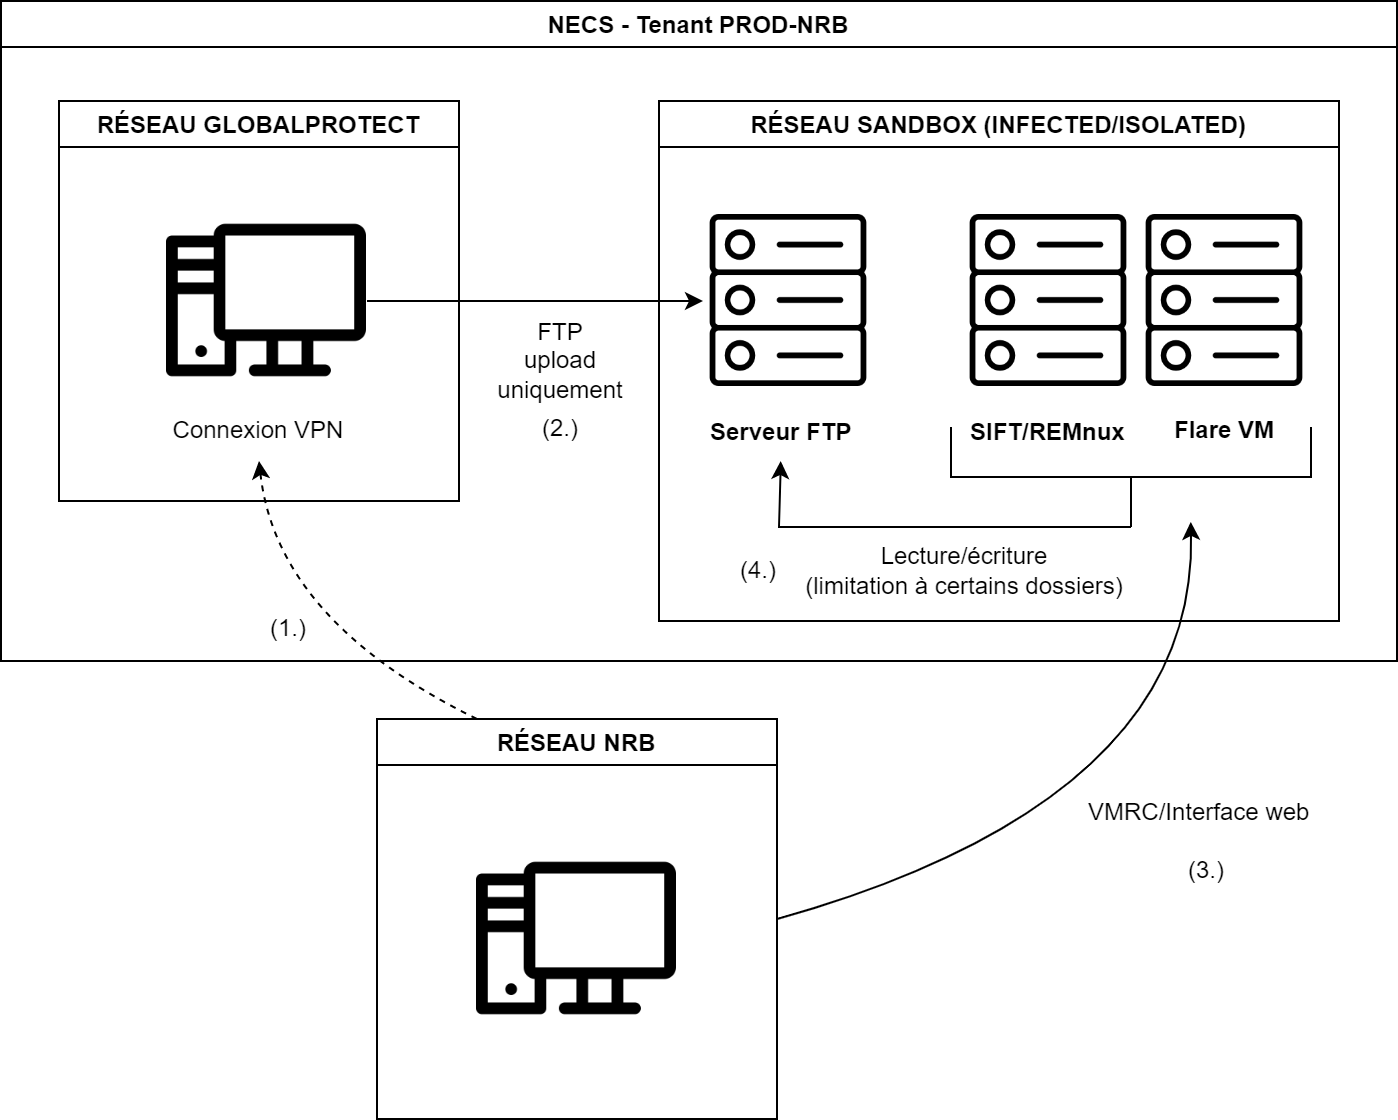
\includegraphics[width=0.95\linewidth]{images/infra-sandbox/infra-sandbox-simplified-01.png}
        }
    }
    \caption{Architecture simplifiée avec les étapes précédant l'analyse.}
    \label{fig:architecture-sandboxing-simplified}
\end{figure}

Avant de pouvoir lancer l'analyse d'un malware ou de données forensiques, il faut bien sûr amener les données sur les machines d'analyse en passant par le serveur FTP. Les quatre étapes à accomplir sont donc:

\begin{enumerate}
    \item Se connecter en VPN (avec le VPN GlobalProtect) sur le réseau NECS.
    \item Uploader les données vers le serveur FTP avec l'utilisateur \textit{upload}.
    \item Se connecter aux machines d'analyse via VMRC (VMWare Remote Console) ou l'interface web (NECS possède la possibilité d'accéder à l'interface graphique de la machine virtuelle via une interface web).
    \item Depuis la machine d'analyse, aller chercher les éléments à analyser en FTP.
\end{enumerate}

Le fait qu'il y ait autant d'étapes n'est pas un problème quand on veut effectuer une analyse forensique de temps à autre. Mais c'est une réelle contrainte si on veut seulement réaliser une analyse rapide et automatique de malware, surtout que ça peut arriver souvent. Puisque la plateforme d'analyse de malware FAME et la sandbox CAPE possèdent toutes les deux une interface web, une amélioration proposée est d'ouvrir le port 80 (le port HTTP) du réseau isolé vers le réseau utilisé lorsqu'on se connecte en VPN avec GlobalProtect. C'est cependant plus risqué d'un point de vue de la cybersécurité parce que le protocole HTTP est souvent utilisé par les malwares.

Évidemment, quand on crée un réseau isolé d'internet, on ne peut plus mettre à jour les machines qui s'y trouvent. Alors pour pouvoir quand même se connecter à internet et effectuer les mises à jour ou installer des nouveaux outils, il y a un deuxième réseau qui a été créé au sein du tenant: le réseau de management. Vous pouvez le voir sur la gauche de la figure \ref{fig:architecture-sandboxing}. L'idée initiale était qu'après l'installation des machines virtuelles, un template de la machine allait être créé afin de pouvoir en générer des nouvelles à volonté. Ensuite, quand on décide de faire une mise à jour, il suffit de recréer la machine à partir du template dans le réseau de management, réaliser les mises à jour et écraser le template avec cette nouvelle machine. Il y aurait toujours des snapshots de machines prêtes pour l'analyse dans le réseau isolé au cas où il faut lancer une analyse sans attendre. Mais les templates auraient été au cœur du système pour créer plusieurs machines lorsque plusieurs analystes doivent effectuer des analyses en même temps ou pour les mises à jour. Malheureusement, il y a eu des problèmes avec la création de templates parce que les machines d'analyse sont très spécifiques (par exemple: une Windows 10 au lieu d'une Windows Server), ce qui fait que pour faire les mises à jour, il faut d'abord restaurer la machine virtuelle à partir de sa snapshot, la déplacer dans le réseau de management avant de faire les mises à jour.

\begin{figure}
    \centering
    \makebox[\textwidth]{
        \resizebox{19cm}{!}{
            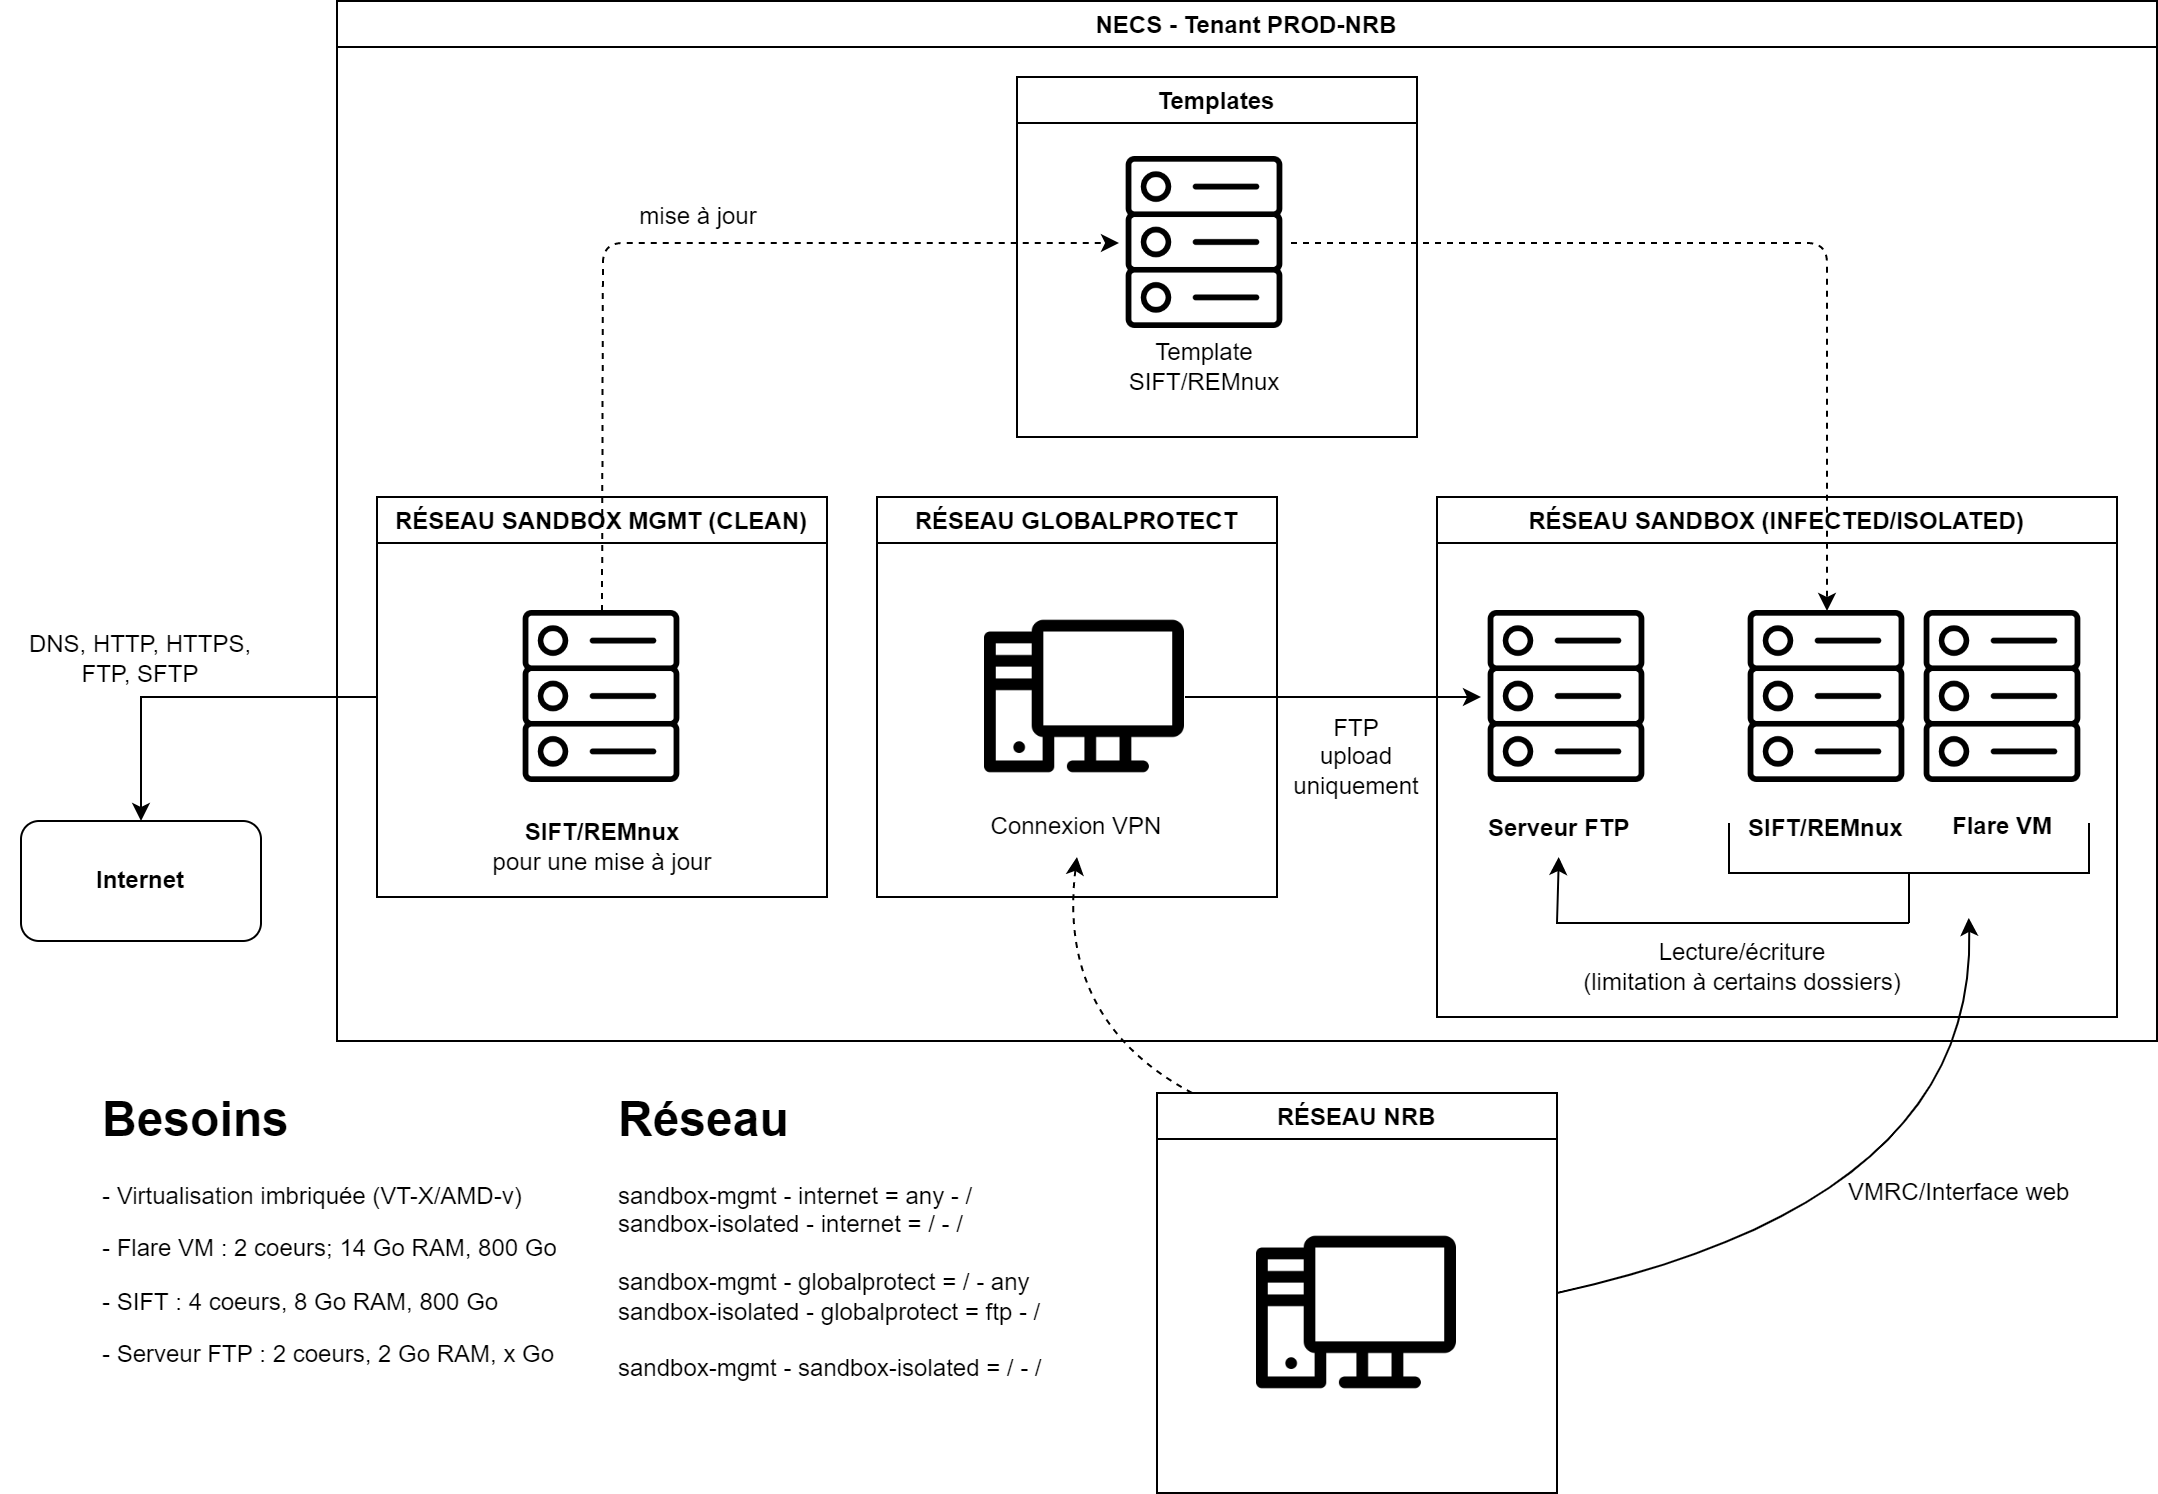
\includegraphics[width=0.95\linewidth]{images/infra-sandbox/infra-sandbox.png}
        }
    }
    \caption{Architecture de la solution d'analyse forensique et de malwares.}
    \label{fig:architecture-sandboxing}
\end{figure}




% LTeX: language=fr

\chapter{Implémentation de la solution}





\section{Serveur FTP}

Pour éviter qu'un utilisateur puisse télécharger un malware depuis l'extérieur par inadvertance, l'organisation du système de fichier a dû être réfléchie en profondeur. Il y a deux utilisateurs: \textit{upload} et \textit{analysis} qui ont chacun leur dossier comme vous pouvez le voir sur la figure \ref{fig:ftp-folders}. Ils ne peuvent pas exécuter la moindre commande sur le serveur, ils sont restreints à la seule utilisation du serveur FTP. En autorisant l'utilisateur upload uniquement à modifier le contenu de son dossier (il n'a même pas le droit de lire les fichiers qu'il contient), on empêche effectivement la possibilité que des malwares puissent sortir du réseau isolé.

% \begin{customquote}
% \begin{verbatim}
% /ftp/
% ├─ d rwx --- ---       analysis analysis  ./analysis/ <== analysis = tout, upload = /
% │     └─ - --- r-- --- analysis analysis  ./fichier   <== analysis = tout, upload = /
% └─ d rwx r-s ---       upload analysis    ./upload/   <== analysis = lecture, upload = tout
%       └─ - --- r-- --- upload analysis    ./fichier   <== analysis = lecture, upload = écriture
% \end{verbatim}
% \end{customquote}

\begin{figure}
    \centering
    \makebox[\textwidth]{
        \resizebox{17cm}{!}{
            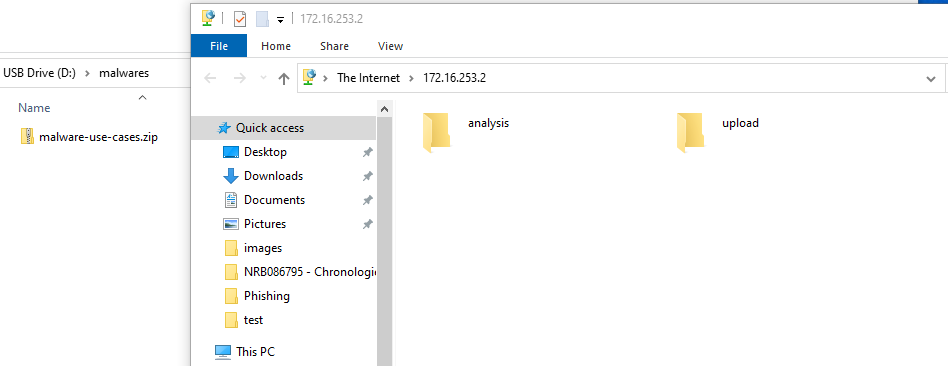
\includegraphics[width=0.95\linewidth]{images/infra-sandbox/ftp-folders.png}
        }
    }
    \caption{Structure de fichiers du serveur FTP.}
    \label{fig:ftp-folders}
\end{figure}





\section{SIFT/REMnux}

Dans cette machine virtuelle d'analyse basée sur Ubuntu qui a été installée à partir de SIFT, il faut bien sûr rajouter la distribution REMnux par-dessus, ce qui se fait facilement puisqu'il suffit de télécharger l'exécutable remnux depuis le répertoire GitHub du projet. Ensuite, il faut installer la plateforme d'analyse automatique de malware FAME et la sandbox CAPE à partir de leurs répertoires GitHub. Pour que FAME puisse communiquer correctement avec CAPE, il a fallu modifier le module FAME qui communiquait avec la sandbox Cuckoo dont CAPE est un fork, c'est-à-dire une copie modifiée.

Ensuite, comme vous pouvez le voir sur la figure \ref{fig:virt-manager}, une machine virtuelle Windows 10 imbriquée a été installée à l'intérieur de SIFT/REMnux. Cette machine imbriquée peut être réinitialisée à volonté par CAPE pour analyser des malwares dans un environnement sain. Pour éviter d'avoir du bruit parasite dans les rapports fournis par CAPE, comme une communication vers un domaine Microsoft parce que le système d'exploitation cherche si des mises à jour sont disponibles, autrement dit: pour avoir moins de faux positifs, il a fallu arrêter plusieurs services et configurer Windows pour arrêter ce genre de requêtes.

\begin{figure}[H]
    \centering
    \makebox[\textwidth]{
        \resizebox{14cm}{!}{
            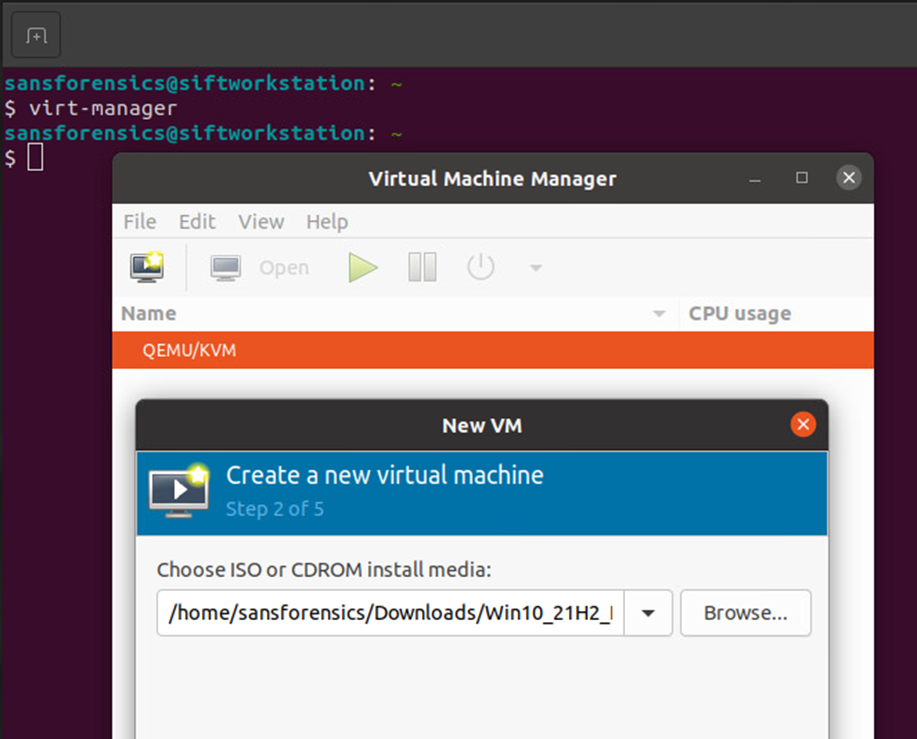
\includegraphics[width=0.95\linewidth]{images/infra-sandbox/install-virt-manager.png}
        }
    }
    \caption{Création d'une machine virtuelle Windows 10 imbriquée pour la sandbox.}
    \label{fig:virt-manager}
\end{figure}





\section{FLARE VM}

L'installation de cette machine virtuelle d'analyse basée sur Windows est très simple. Tout d'abord, on peut télécharger une machine virtuelle Windows de test fournie par Microsoft. Ensuite, il suffit de télécharger un script PowerShell sur le répertoire GitHub du projet et de l'exécuter avec des privilèges administrateurs. Ce script va apporter toutes les modifications nécessaires au système d'exploitation et installer presque tous les outils dont nous avons besoin. Il en manque seulement quelques-uns, en particulier des logiciels qui ne sont pas open source comme ArsenalImageMounter et Kape.




% LTeX: language=fr

\chapter{Réflexion sur les Procédures}










\section{Acquisition forensique}

L'acquisition forensique est divisée en trois parties: la préparation, l'acquisition des données en elle-même et la phase de post-acquisition. La préparation est se déroule à la fois longtemps avant de lancer l'acquisition forensique comme en installant les logiciels, mais aussi juste avant, en récupérant les identifiants du compte administrateur local de la machine, par exemple. Après avoir effectué l'acquisition, vient la phase de post-acquisition lors de laquelle, on va préparer ce qui vient ensuite: l'analyse des données forensiques.





\subsection{Préparation}

La \textit{préparation} commence longtemps avant l'acquisition des données forensiques. D'abord, au point de vue hardware, il faut obtenir des disques durs externes suffisamment grands pour pouvoir contenir les données des machines dont on veut faire l'analyse forensique. Il faut aussi qu'ils soient assez rapide pour essayer de gagner un maximum de temps lors de la copie des données sur le disque externe, c'est pour cela que la technologie SSD est recommandée, tout comme les dernières versions des connecteurs USB.

\begin{example}
    \hspace{0.45cm} Par exemple, pour un PC avec un disque dur de 256 Go et 8 Go de mémoire RAM, on pourrait penser qu'un disque dur externe de seulement 264 Go suffit. C'est cependant faux. La mémoire RAM qui sera acquise est plus grande que 8 Go à cause du swap, qui est le stockage d'une partie de la mémoire volatile sur le disque. De plus, il faut aussi suffisamment de place pour y mettre les outils dans le cas où la machine à analyser n'aurait qu'un seul port USB.
\end{example}

Un autre point qui est lié à la \textit{préparation} est l'isolement de la machine infectée du réseau. On peut facilement le faire avec Microsoft EDR (voir figure \ref{fig:microsoft-edr-isolate}). Le problème ne vient cependant pas toujours d'un malware qui aurait infecté le PC d'un utilisateur, mais il peut venir de l'utilisateur lui-même, par exemple parce qu'il aurait agi de manière répréhensible et voudrait en effacer les traces. Microsoft EDR ne permet pas de bloquer l'utilisateur pour l'empêcher d'accéder à son PC. 

\begin{figure}
    \centering
    \makebox[\textwidth]{
        \resizebox{9cm}{!}{
            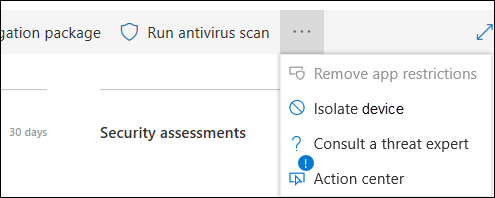
\includegraphics{images/incident-response/microsoft-edr-isolate.png}
        }
    }
    \caption{Isolation d'un appareil infecté dans Microsoft EDR pour empêcher l'infection de s'étendre dans le réseau.}
    \label{fig:microsoft-edr-isolate}
\end{figure}

Si on peut modifier à la fois l'AD et la machine de l'utilisateur, il y a bien moyen de le bloquer quand même. Pour l'empêcher d'effacer ses données à distance malgré tout, on devra:

\begin{enumerate}
    \item Désactiver l'utilisateur ou modifier son mot de passe dans l'AD pour empêcher l'utilisateur de se reconnecter à partir de l'AD.
    \item Supprimer le hash de son mot de passe stocké localement dans l'ordinateur pour empêcher l'utilisateur de se reconnecter localement.
    \item Déconnecter l'utilisateur à distance.
\end{enumerate}

Comme cela sortait un peu du cadre de mon TFE, je me suis arrêté après avoir testé que cette méthode fonctionnait bien mais je n'ai pas écrit de procédure complète sur son utilisation.

En bref, la phase de préparation consiste en la préparation matérielle et logicielle pour que l'acquisition forensique se passe au mieux au moment où en a besoin. De plus, dans les premiers instants de la réponse à incident, la préparation à l'acquisition forensique, en isolant les machines infectées et en obtenant les identifiants d'un compte administrateur local sur chacune des machines à analyser est essentiel pour ne pas perdre de temps lorsque l'analyste sera en leur possession.





\subsection{Mémoire volatile}

L'\textit{acquisition des données volatiles} doit se faire dès que l'analyste forensique a accès à la machine à analyser. D'ailleurs, selon le NIST, il faut décider à l'avance si on acquerra les données volatiles ou pas parce que le temps perdu à le décider fait qu'on risque de perdre des informations importantes. \cite{5} Au moins, la procédure pour les récupérer est plutôt simple puisqu'il suffit, après avoir brancher un disque dur externe contenant l'outil d'acquisition choisi, ici: Belkasoft RAM Capture, puis le lancer en tant qu'administrateur et choisir le lieu où la copie de la RAM doit être enregistré (voir figure \ref{fig:belkasoft-ram-capture}).

\begin{figure}
    \centering
    \makebox[\textwidth]{
        \resizebox{11cm}{!}{
            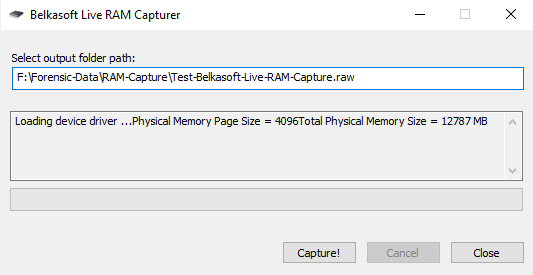
\includegraphics{images/RAM/ram-capture-01.png}
        }
    }
    \caption{Capture RAM avec Belkasoft RAM Capture.}
    \label{fig:belkasoft-ram-capture}
\end{figure}





\subsection{Mémoire de masse}

L'\textit{acquisition des données non-volatiles} est la troisième étape et se fait avec FTK Imager, qu'il faut bien sûr lancer avec des privilèges administrateur. C'est l'étape la plus longue, et sa vitesse dépend de deux facteurs: la rapidité en écriture sur le disque dur externe et de la vitesse de transfert qui dépend du type de transfert utilisé. Par exemple, un SSD utilisant un port USB 3.0 sera bien plus rapide qu'un simple disque dur utilisant la technologie USB 2.0.

Si le disque à analyser est chiffré avec BitLocker, il faut absolument récupérer la clé de chiffrement. Dans la plupart des organisations, elle sera enregistrée dans l'Active Directory. Si ce n'est pas le cas, on peut toujours la récupérer en ligne de commande avec: \texttt{manage-bde -protectors <lettre-de-lecteur> -get}. Cette commande doit être lancée avec des privilèges administrateurs, son utilisation est expliquée plus en détail dans la section sur les outils d'acquisition de données forensiques non-volatiles.





\subsection{Clé USB}

Lorsqu'on doit effectuer l'analyse forensique d'une clé USB, il faut, comme pour l'image disque, utiliser FTK Imager en tant qu'administrateur. Le problème de la clé USB est que dès qu'on la branche, on va commencer à modifier des données qui s'y trouvent parce que Windows va aller lire des données qui y sont présentes. Il y a deux solutions pour y remédier. La première est d'utiliser un élément hardware \textit{write-blocker} qui se place entre le port USB de l'ordinateur et la clé USB pour éviter de manière physique qu'on aille modifier des données. La seconde possibilité est de monter la clé USB en lecture seule en modifiant un paramètre Windows. Celui-ci se trouve dans le registre comme vous pouvez le voir sur la figure \ref{fig:usb-key-read-only} et il nécessite des droits administrateurs pour être modifié. \cite{12} Des tests ont été effectués dans le cadre du stage pour vérifier qu'une fois que ce changement est effectué, aucune modification quelle qu'elle soit ne sera apportée sur la clé USB.

\begin{figure}
    \centering
    \makebox[\textwidth]{
        \resizebox{19cm}{!}{
            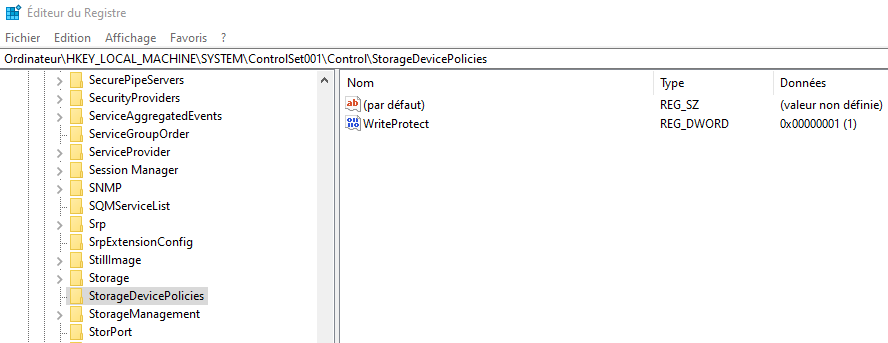
\includegraphics{images/Disque/read-only-registry.png}
        }
    }
    \caption{Modification d'une clé de registre pour monter une clé USB en lecture seule.}
    \label{fig:usb-key-read-only}
\end{figure}





\subsection{Post-acquisition}

La dernière étape est la \textit{post-acquisition}. Il s'agit de faire des copies pour pouvoir effectuer les analyses tout en cherchant à ne pas modifier les données. En plus de copier les données, on calcule aussi les hashs des données juste après l'acquisition pour montrer que les analystes n'ont pas modifié les données que ce soit volontairement ou par accident.










\section{Analyse de menaces}

\begin{figure}
    \centering
    \makebox[\textwidth]{
        \resizebox{16cm}{!}{
            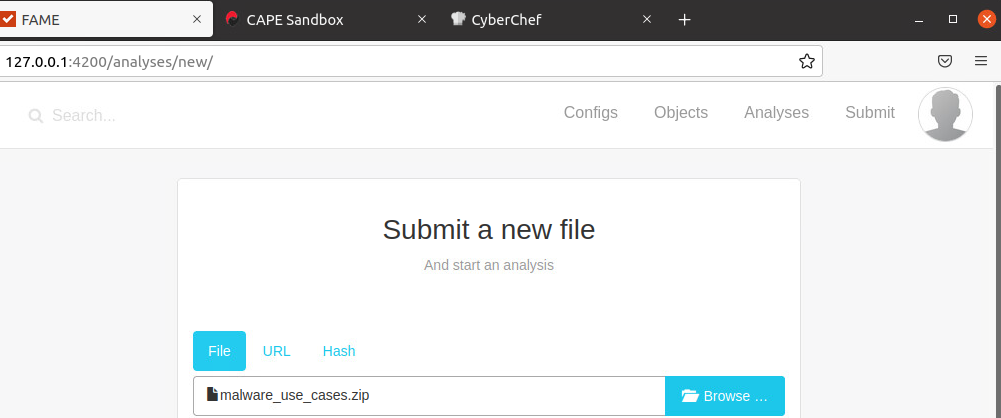
\includegraphics{images/malware/fame-submit.png}
        }
    }
    \caption{Interface de soumission de FAME.}
    \label{fig:fame-submission}
\end{figure}

La marche à suivre pour analyser un malware ou tout autre document supposé malicieux est simple grâce aux outils automatiques mis en place comme la plateforme d'analyse automatique de malwares FAME et la sandbox CAPE qui effectue des analyses dynamiques de malware dans une machine virtuelle imbriquée. Le seul souci est qu'il faut transférer le fichier à analyser depuis le PC de l'analyste vers la plateforme d'analyse qui se trouve dans un réseau isolé. Ceci a été expliqué plus en détail plus haut dans la section sur l'architecture de la solution. En résumé, il faut: se connecter en VPN au tenant NECS (NECS est le cloud NRB où est hébergée l'infrastructure), se connecter au serveur FTP pour y uploader le fichier à analyser, se connecter avec VMRC (VMWare Remote Console) à une machine d'analyse et télécharger le fichier en FTP depuis là pour lancer l'analyse via l'interface web (figure \ref{fig:fame-submission}).

L'analyse se fait de manière automatique. Par exemple, quand on soumet un mail qui a été signalé comme phishing par un utilisateur, une analyse de ses headers va être effectuée, les pièces jointes seront extraites et analysées à leur tour. On peut voir l'analyse des headers d'un de mes use cases sur la figure \ref{fig:fame-email-headers}. Grâce à cette analyse, on peut voir que le nom de domaine qui l'a envoyé est utilisé par un service de boîtes mails temporaires que l'on pourrait décider de bannir pour prévenir ce genre d'attaques à l'avenir.

\begin{figure}
    \centering
    \makebox[\textwidth]{
        \resizebox{19cm}{!}{
            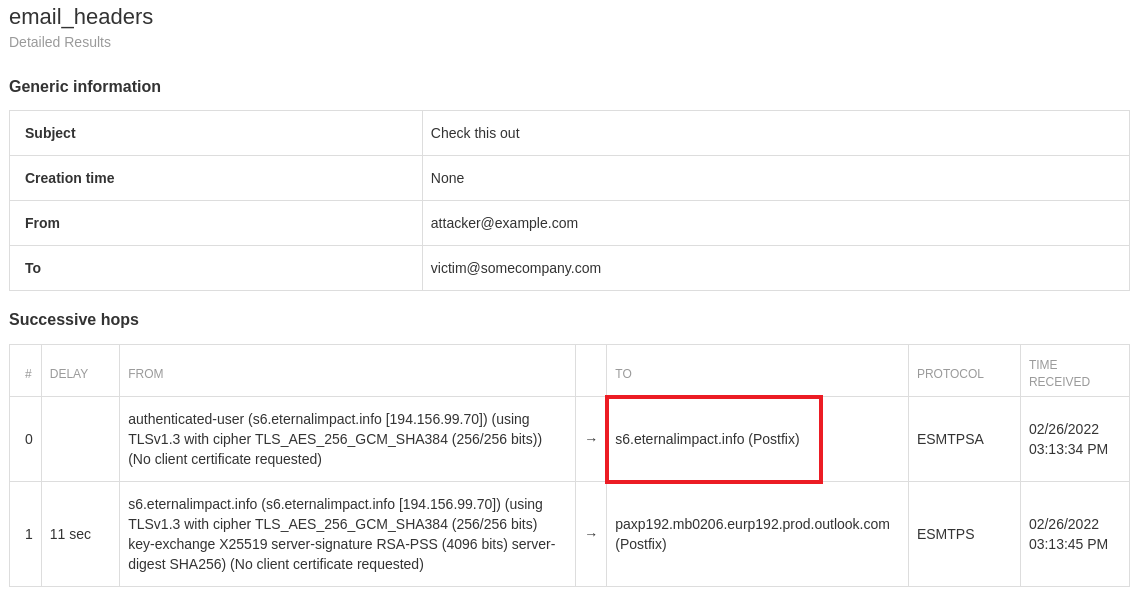
\includegraphics{images/malware/fame-analysis-11.png}
        }
    }
    \caption{Analyse des headers d'un email montrant que l'envoyeur est un service d'adresses email temporaires.}
    \label{fig:fame-email-headers}
\end{figure}

Dans le cas où les informations disponibles depuis l'interface de FAME en rapport avec l'analyse dynamique ne suffiraient pas, on peut toujours entrer plus dans le détail en cliquant sur \textit{View Report} comme sur la figure \ref{fig:fame-cape-report}. On arrive alors sur l'interface web de CAPE qu'on peut voir sur la figure \ref{fig:cape-analysis}.

\begin{figure}
    \centering
    \makebox[\textwidth]{
        \resizebox{17cm}{!}{
            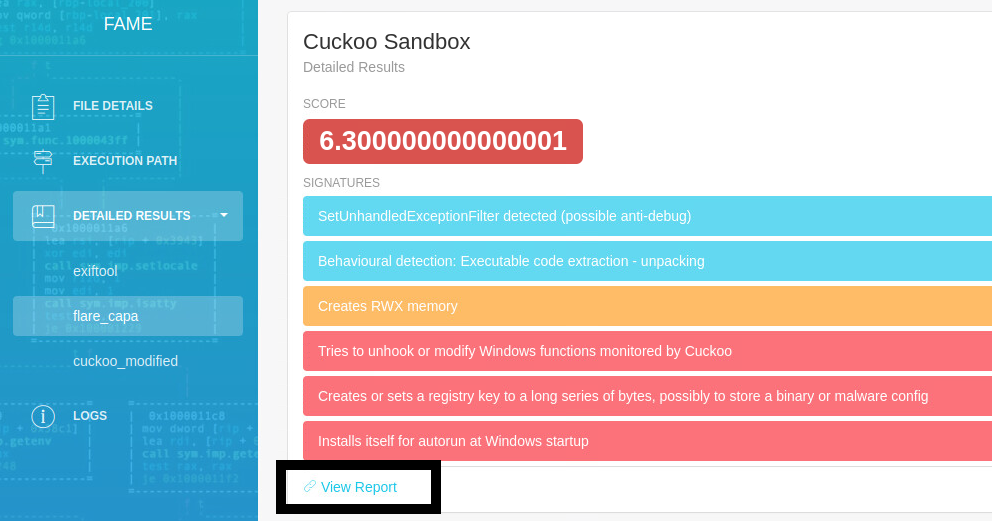
\includegraphics{images/malware/fame-analysis-09-report.png}
        }
    }
    \caption{Interface de résultats de FAME montrant les résultats des modules lancés, ici, CAPE Sandbox - dérivée de Cuckoo.}
    \label{fig:fame-cape-report}
\end{figure}

Sur l'interface web de CAPE, on peut voir les résultats de manière beaucoup plus précise et aussi en bien plus grande quantité. Par exemple, sur la figure \ref{fig:cape-analysis}, on peut voir non seulement que des tâches Windows ont été créées mais aussi lesquelles. On peut aussi y télécharger des fichiers. Il y a les fichiers qui ont été créés par le malware, un dump réseau qui contient tous les paquets qui ont transité sur le réseau en provenance et à destination de la sandbox, ainsi qu'un dump de la mémoire RAM de la machine virtuelle imbriquée infectée.

\begin{figure}
    \centering
    \makebox[\textwidth]{
        \resizebox{17cm}{!}{
            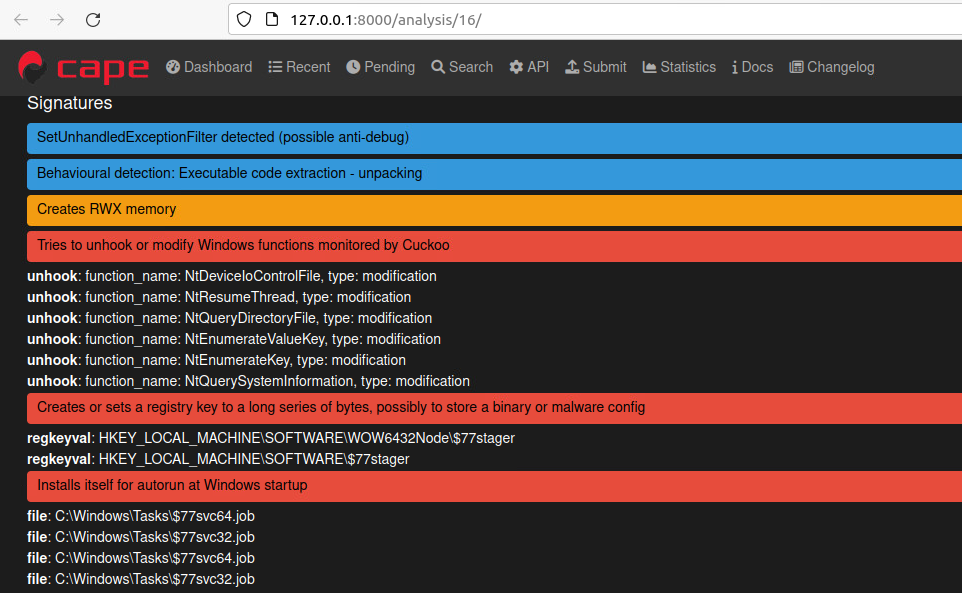
\includegraphics{images/malware/cape-analysis-02.png}
        }
    }
    \caption{Analyse du comportement du malware plus en détail avec CAPE Sandbox.}
    \label{fig:cape-analysis}
\end{figure}










\section{Analyse forensique}





\subsection{Extraire les données}

Pour analyser les informations présentes sur l'image d'un disque, il faut lancer plusieurs actions comme scanner les espaces vides du disque pour trouver des fichiers supprimés, copier les fichiers de grande importance forensique ou encore les parser pour normaliser l'information, ce qui rend l'analyse plus aisée. Mais la première chose à faire est de déchiffrer les données le cas échéant. Dans le cas d'un disque chiffré avec BitLocker, il faut monter l'image disque avec \textit{Arsenal Image Mounter} (figure \ref{fig:arsenal-image-mounter}). On peut ensuite la déchiffrer directement avec la clé dans l'explorateur de fichiers comme sur la figure \ref{fig:bitlocker}.

Après avoir monté l'image, on va en extraire les fichiers qui ont une importance forensique et normaliser les données de ces fichiers avec \textit{Kape}, un outil créé par l'entreprise Kroll. Il faut lancer le logiciel avec des privilèges administrateur pour qu'il puisse lire les fichiers systèmes. Vous pouvez voir l'interface graphique de Kape appelée \textit{gkape} (figure \ref{fig:gkape}). Elle est divisée en deux parties:

\begin{itemize}
    \item La partie \textit{Target} sert à configurer les extractions de fichiers de l'image montée pour en placer des copies dans un dossier. Quelques exemples de fichiers sont les logs, les registres, la MFT (Master File Table, l'index principal du système de fichiers NTFS, utilisé par Windows), etc.
    \item La partie \textit{Module} sert à configurer le parsing des données extraites, par exemple en transformant les logs au format CSV et en les regroupant sous un seul fichier ou en transposant les données stockées dans la MFT au format CSV.
\end{itemize}

\begin{figure}
    \centering
    \makebox[\textwidth]{
        \resizebox{19cm}{!}{
            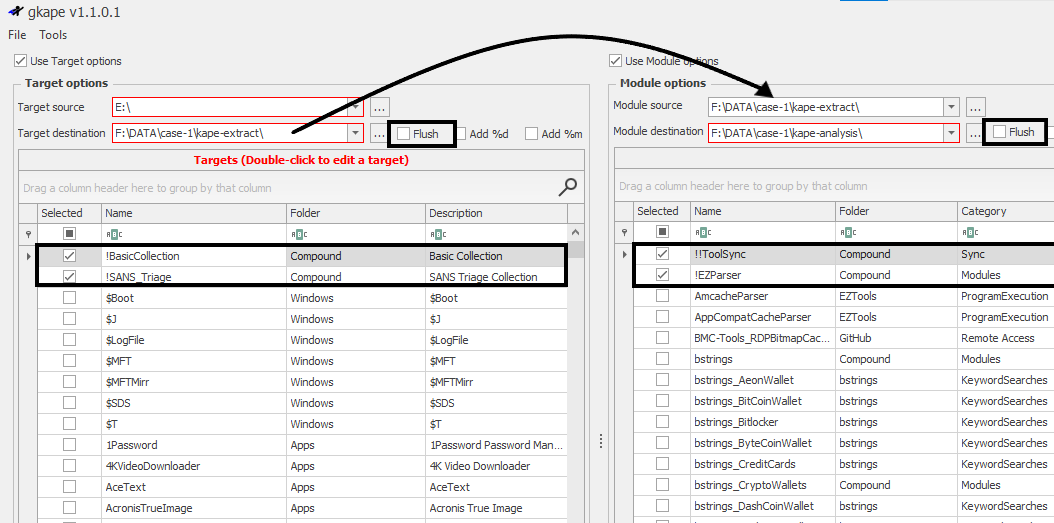
\includegraphics{images/Disque/kape-03.png}
        }
    }
    \caption{Interface graphique de Kape: \textit{gkape}.}
    \label{fig:gkape}
\end{figure}


\textit{Autopsy} est un logiciel d'analyse disque qui va nous permettre d'analyser les espaces vides de l'image disque pour voir s'il n'y a pas de fichiers supprimés qui s'y trouveraient. Il faut lancer ce programme avec des privilèges administrateur si l'image a été montée, mais si on analyse le fichier qui est l'image disque, on n'en a pas besoin (ça dépend donc de si le disque est chiffré ou non). En plus de cela, Autopsy possède une série de modules qui vont aller scanner les fichiers pour en extraire de l'information intéressante (voir figure \ref{fig:autopsy-ingest}). Les modules les plus intéressants sont:

\begin{itemize}
    \item \textit{Recent Activity}: il recherche les documents récents, les programmes installés, les données du navigateur comme les comptes enregistrés, l'historique de navigation et les favoris.
    \item \textit{File Type Identification}: il identifie le type des fichiers en fonction de leur signature.
    \item \textit{Extension Mismatch Detector}: il liste les documents dont l'extension ne correspond pas à leur type. Par exemple, un exécutable avec une extension \textit{.txt} se ferait détecter par ce module.
    \item \textit{Email Parser}: il liste les emails enregistrés localement sur l'ordinateur.
    \item \textit{Encryption Detection}: il va chercher les fichiers qui ont une entropie élevée, ce qui est indicateur d'un chiffrement.
    \item \textit{Interesting File Identifier}: ce module aurait peut-être dû être nommé \textit{Interesting Programs Identifier} parce qu'il va chercher les programmes intéressants comme les logiciels de chiffrement, les VPN, les crypto wallets, etc.
\end{itemize}

Les modules \textit{Embedded File Extractor} et \textit{Virtual Machine Extractor} peuvent être très utiles mais ils peuvent prendre énormément de temps. Ce n'est donc pas à activer en toutes circonstances.

\begin{figure}
    \centering
    \makebox[\textwidth]{
        \resizebox{17cm}{!}{
            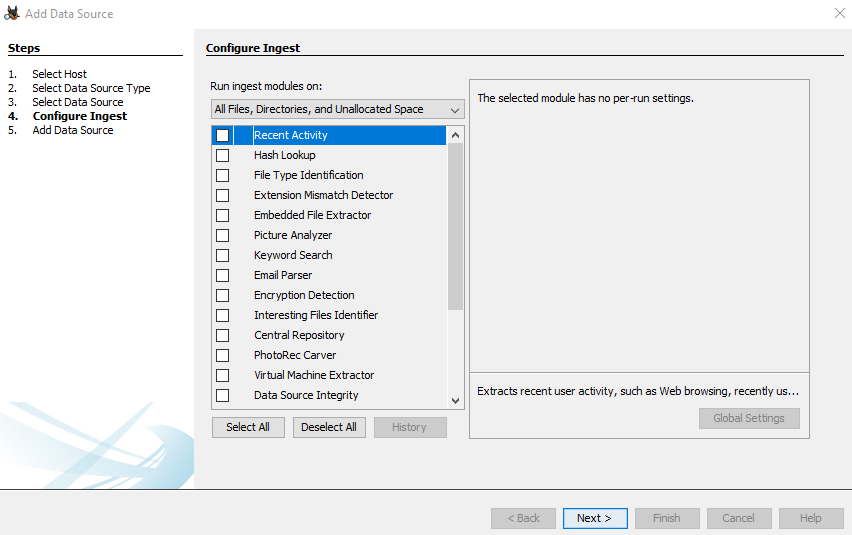
\includegraphics{images/Disque/autopsy-07.png}
        }
    }
    \caption{Ensemble de modules d'Autopsy qui peuvent être lancés pour analyser une image disque.}
    \label{fig:autopsy-ingest}
\end{figure}


\textit{Thor Lite} est un scanner anti-virus qu'il faut lancer en tant qu'administrateur. Ses résultats sont faciles à analyser. On peut le lancer avec la commande suivante: \texttt{.$\backslash$thor64-lite.exe -{}-intense -a FileSystem -{}-path E:$\backslash$ -o .$\backslash$output$\backslash$}





\subsection{Analyse des données}



\subsubsection{Analyse de logs}

\textit{Chainsaw} est un outil d'analyse de logs Windows (au format evtx) qui liste les évènements suspicieux, et en particulier, tout ce qui est lié au mouvement latéral. La première chose à faire avant de l'utiliser est de trouver le dossier contenant les logs extraits par Kape. Les logs sont normalement stockés dans le dossier \texttt{C:$\backslash$Windows$\backslash$System32$\backslash$winevt$\backslash$logs$\backslash$}. Si on les a extraits avec Kape et pas manuellement, ils devraient se trouver dans un dossier comme \\
\texttt{E:$\backslash$DATA$\backslash$case-1$\backslash$kape-extract$\backslash$F$\backslash$Windows$\backslash$System32$\backslash$winevt$\backslash$logs$\backslash$} \\
Ensuite, on peut lancer chainsaw avec peu de règles pour commencer, afin d'avoir une première vue sur les données. On pourra ensuite l'utiliser avec plus de règles pour avoir une vue complète et obtenir toutes les alertes. On peut le faire avec les commandes suivantes:

\begin{enumerate}
    \item Vue d'ensemble: \texttt{.$\backslash$chainsaw.exe hunt <dossier-logs> -{}- lateral-all}
    \item Appliquer toutes les règles: \\
    \texttt{.$\backslash$chainsaw.exe hunt <dossier-logs> -{}- lateral-all \\
    -{}-rules .$\backslash$sigma\_rules$\backslash$ \\
    -{}-mapping .$\backslash$mapping\_files$\backslash$sigma-mapping.yml}
\end{enumerate}

Sur la figure \ref{fig:chainsaw-lateral-movement}, on peut voir que chainsaw a récupéré toutes les connexions à distances effectuées sur la machines. Ces évènements peuvent être indicateurs de mouvement latéral vers la machine.

\begin{example}
    \hspace{0.45cm} Par exemple, un attaquant pourrait avoir créé une tâche à distance sur la machine pour l'infecter, ce qui aurait généré à la fois un log de connexion à distance et un log de création de tâche. En analysant les évènements autour de ces connexions réseau, on peut trouver des traces de mouvement latéral, ce qui peut conduire à une escalade dans la réponse à incident.
\end{example}

\begin{figure}
    \centering
    \makebox[\textwidth]{
        \resizebox{16cm}{!}{
            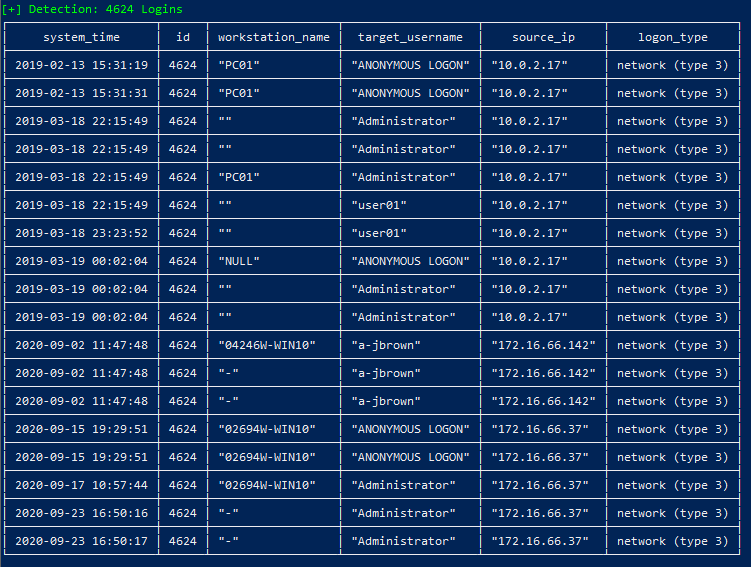
\includegraphics{images/Disque/chainsaw-02.png}
        }
    }
    \caption{Analyse des connexions à distance indiquant des possibles mouvements latéraux avec chainsaw.}
    \label{fig:chainsaw-lateral-movement}
\end{figure}



\subsubsection{Analyse des fichiers intéressants d'un point de vue forensique}

Les outils pour analyser les fichiers intéressants d'un point de vue forensique ont été créés par Erik Zimmerman, qui travaille chez Kroll, l'entreprise qui a créé Kape. Les trois plus intéressants sont \textit{Registry Explorer} et \textit{Timeline Explorer}, mais je vais présenter aussi \textit{Shellbags Explorer} dans cette section.

\textit{Registry Explorer} permet de lire les clés de registres et même de les corriger avec les logs si elles sont \textit{sales} (comme une base de données corrompue qu'on peut nettoyer grâce aux logs). C'est très utile de pouvoir naviguer dans le registre pour y retrouver des données. Par exemple, sur la figure \ref{fig:zimmerman-registry-explorer}, on peut voir la date à laquelle une clé USB a été branchée pour la première fois. Dans le cas où un PC a été infecté par une clé USB, ça peut aider à trouver la date d'infection.

\begin{figure}
    \centering
    \makebox[\textwidth]{
        \resizebox{19cm}{!}{
            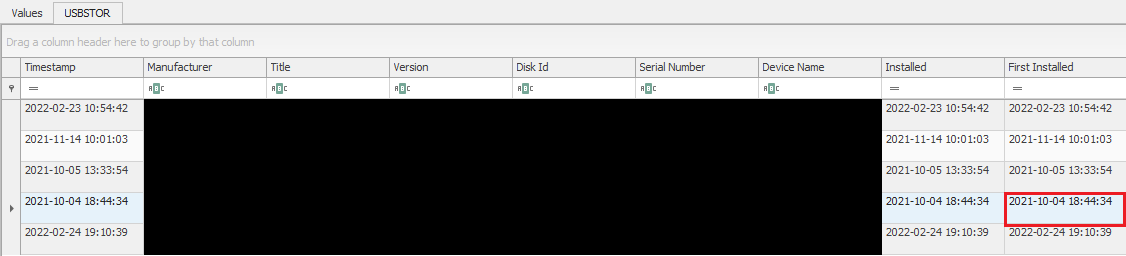
\includegraphics{images/Disque/zimmerman-02.png}
        }
    }
    \caption{Analyse des registres avec Registry Explorer pour trouver quand une clé USB a été branchée pour la première fois.}
    \label{fig:zimmerman-registry-explorer}
\end{figure}

\textit{Timeline Explorer}, c'est un peu un substitut à Excel que l'on peut utiliser pour analyser les fichiers CSV générés par Kape. Bien qu'il ait beaucoup moins de fonctionnalités qu'Excel, il peut analyser des fichiers beaucoup plus gros aisément et ne requiert pas de licence. On peut, par exemple, analyser les données de la MFT, des registres ou encore des preuves d'exécution de programmes compilées par Kape. Sur la figure \ref{fig:zimmerman-timeline-explorer}, vous pouvez voir l'analyse de la MFT d'un PC infecté par un malware qui a modifié la date de création \textit{Created0x10} de ses fichiers pour faire croire qu'ils avaient étés créés en 2019 ou lieu de 2022. Ce timestamp est accessible via l'API Win32 mais la MFT utilise un deuxième timestamp pour la création des fichiers: le \textit{Created0x30}, qui n'est accessible que par le kernel Windows et n'a donc pas été modifié par le malware.

\begin{figure}
    \centering
    \makebox[\textwidth]{
        \resizebox{18cm}{!}{
            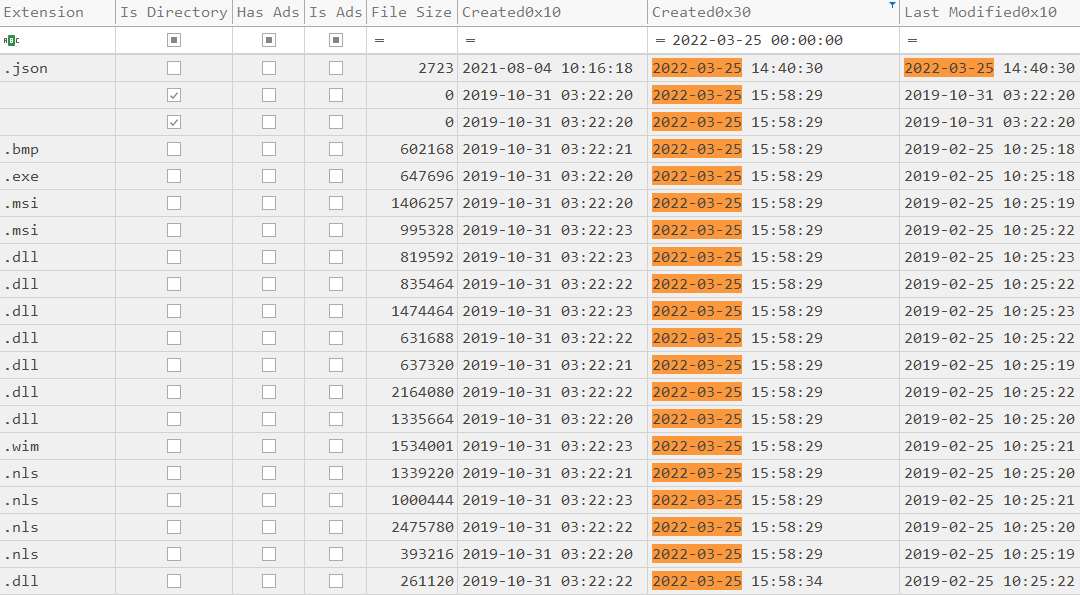
\includegraphics{images/Disque/zimmerman-03.png}
        }
    }
    \caption{Analyse de la MFT avec Timeline Explorer pour trouver les fichiers créés à certaine date malgré que le timestamp ait été modifié.}
    \label{fig:zimmerman-timeline-explorer}
\end{figure}

Quand on visite un dossier avec l'explorateur de fichiers de Windows, on peut modifier l'affichage des fichiers qu'il contient pour les trier en fonction de la date, de l'ordre alphabétique ou encore changer l'affichage pour montrer une miniature des images. Ces paramètres sont enregistrés par Windows pour améliorer l'expérience utilisateur mais permettent aussi à un enquêteur forensique de trouver la preuve qu'un dossier a bel et bien existé et a été visité par un utilisateur.

\textit{Shellbags Explorer} permet, comme son nom l'indique, d'analyser les shellbags. Sur la figure \ref{fig:zimmerman-shellbags-explorer}, vous pouvez voir les dossier consulté par un utilisateur, y compris sur un serveur FTP. En utilisant ces informations, on peut prouver l'existence de serveurs de fichiers personnels et l'existence de dossiers potentiellements sensibles sur ceux-ci.

\begin{figure}
    \centering
    \makebox[\textwidth]{
        \resizebox{19cm}{!}{
            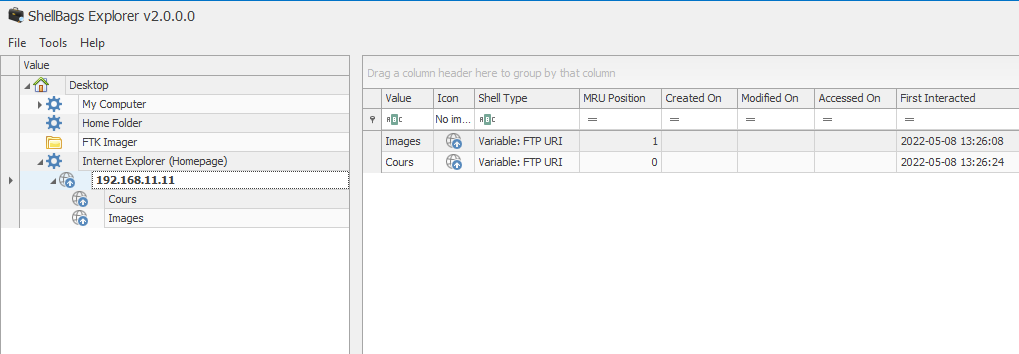
\includegraphics{images/Disque/zimmerman-01.png}
        }
    }
    \caption{Analyse des shellbags avec Shellbags Explorer pour chercher des traces d'exfiltration de données.}
    \label{fig:zimmerman-shellbags-explorer}
\end{figure}

Il faut faire attention aux différence de zones horaires et au changement d'heure. Par exemple, lorsqu'on analyse un système compromis avant le changement d'heure, on aura deux types de données. Premièrement, il y a celles qui sont indépendantes de la configuration de la machine d'analyse, c'est généralement parce que la date et l'heure de l'évènement est stockée directement. Deuxièmement, il y a celles qui ont un timestamp dépendant de la configuration de la machine, comme lorsqu'on utilise \textit{Unix epoch} qui compte le nombre de secondes depuis le 1er janvier 1970 à minuit UTC. Dans ce cas, la date affichée à l'analyste sera dépendante de la zone horaire de sa machine d'analyse puisque la zone horaire de la machine analysée n'est pas contenue dans la donnée.



\subsubsection{Analyse générale du disque}

Avec \textit{Autopsy}, on peut voir la structure du système de fichiers. Cela peut servir pour lire certains fichiers, par exemple, en allant lire le fichier contenant l'historique des commandes powershell. Grâce à l'analyse des fichiers supprimés, on peut aussi retrouver des données qu'un utilisateur a peut-être voulu cacher. Et en cherchant à travers l'historique des documents récents, plutôt que de devoir analyser l'ensemble des documents, il est possible de choisir, une poignée de documents récents à analyser si on suspecte ce vecteur d'infection d'avoir compromis un système. De manière générale, l'enquête sur Autopsy va se faire sur ses données qui ont été rassemblées sous la section \textit{Data Artifacts} que vous pouvez voir sur la figure \ref{fig:autopsy-analysis} qui regroupe un ensemble de données intéressantes.

\begin{figure}
    \centering
    \makebox[\textwidth]{
        \resizebox{16cm}{!}{
            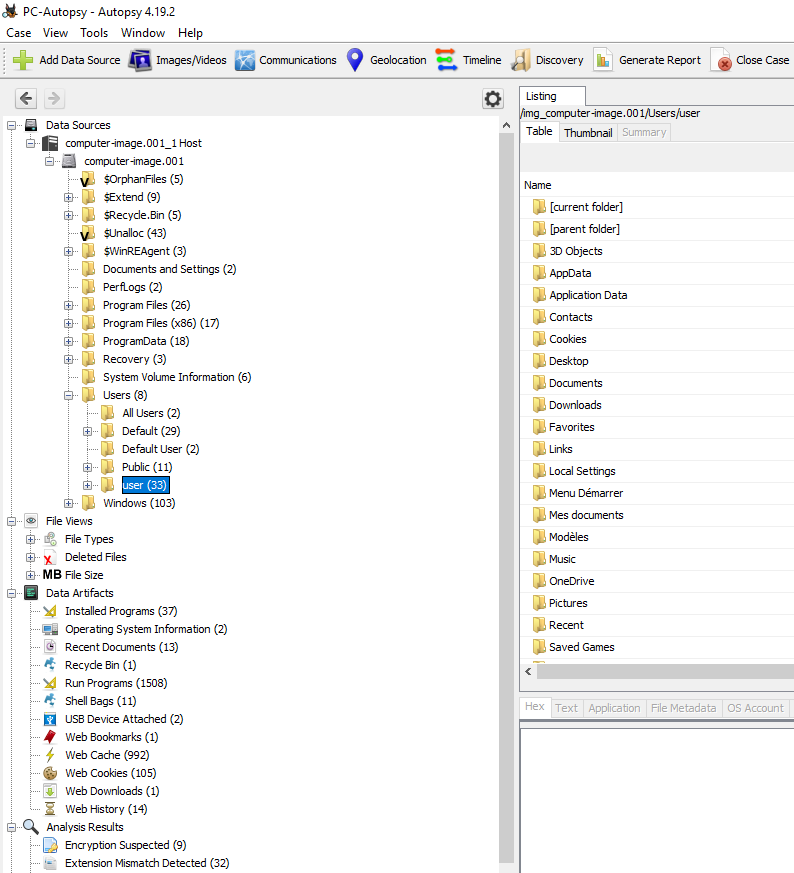
\includegraphics{images/Disque/autopsy-11.png}
        }
    }
    \caption{Analyse d'une image disque avec Autopsy.}
    \label{fig:autopsy-analysis}
\end{figure}





\subsection{Analyse de la mémoire volatile}

L'outil d'analyse de la mémoire volatile utilisé ici est Volatility 2 qui est un framework open source utilisé en ligne de commande en précisant un module. Il existe un ensemble de modules existant, à la fois supportés par le framework et d'autres écrits par la communauté. Un autre point important à soulever est que la mémoire RAM est différente en fonction de la machine dont elle provient. Pour pouvoir analyser un dump mémoire, il faut donc utiliser un profil qui correspond à la machine analysée, par exemple: Windows 10 x64 ou Windows 7 x86. La structure d'une commande dans Volatility contient donc ces deux éléments, le profil et le module en option: \texttt{volatility -f <dump-mémoire> -{}-profile=<trouvé-avec-imageinfo> <module>}

\begin{figure}
    \centering
    \makebox[\textwidth]{
        \resizebox{13cm}{!}{
            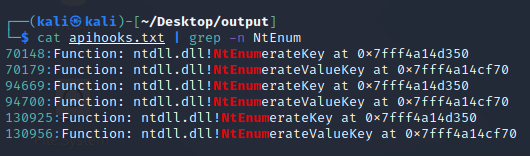
\includegraphics{images/RAM/volatility-rootkit-hooked-functions.png}
        }
    }
    \caption{Fonctions hookées par un rootkit listées avec Volatility.}
    \label{fig:volatility-rootkit}
\end{figure}

La méthode pour analyser un dump mémoire est donc la suivante: \cite{13}

\begin{enumerate}
    \item Identifier le profil de l'image avec: \textit{imageinfo} (à lancer sans l'option \textit{profile}).
    \item Identifier les processus malveillants:
    \begin{itemize}
        \item Lister les processus cachés: processus listés par \texttt{psscan}, mais pas par \texttt{pslist}. La comparaison est facile avec \texttt{psxview} qui affiche un tableau de comparaison.
        \item Chercher un processus "système" qui a un parent anormal: \texttt{pstree}.
        \item Identifier un processus injecté avec la méthode de process hollowing: \texttt{hollowfind}.
        \item Lister les pages mémoires suspectes avec des permissions en écriture et exécution, ce qui permet d'écrire et exécuter du code dans un autre processus par exemple: \texttt{malfind}.
    \end{itemize}
    \item Analyser les artefacts réseau: \textit{netscan}, par exemple l'utilisation du port 4444 est suspecte car c'est le port configuré par défaut par l'outil metasploit.
    \item Chercher la présence d'un rootkit en cherchant des fonctions Windows qui ont été modifiées pour cacher le rootkit:
    \begin{itemize}
        \item Liste des hooks sur les fonctions de l'API Windows: \texttt{apihooks}, vous pouvez voir un exemple sur la figure \ref{fig:volatility-rootkit} que des fonctions servant à lister les clés de registres ont été modifiées par un rootkit pour cacher certaines clés.
        \item Liste des hooks dans le System Service Descriptor Table (la table d'adressage des API): \texttt{ssdt} (exemple de hooks importants: \texttt{<volatility-ssdt> | egrep -v '(ntoskrnl|win32k)'})
    \end{itemize}
    \item Autres données intéressantes à analyser:
    \begin{itemize}
        \item Afficher l'historique des commandes: \textit{cmdscan}, ce n'est pas stocké sur le disque, c'est donc la seule manière de l'obtenir.
        \item Lister des clés intéressantes dans les registres: \textit{autoruns} et \textit{userassist}, vous pouvez voir un exemple sur la figure \ref{fig:volatility-userassist} où on voit la preuve que l'exécutable \textit{Install.exe} a été exécuté.
        \item Liste des services: \textit{svcscan}.
        \item Extraire un processus, une librairie ou un driver: \textit{procdump}, \textit{dlldump}, \textit{moddump}.
    \end{itemize}
\end{enumerate}

\begin{figure}
    \centering
    \makebox[\textwidth]{
        \resizebox{16cm}{!}{
            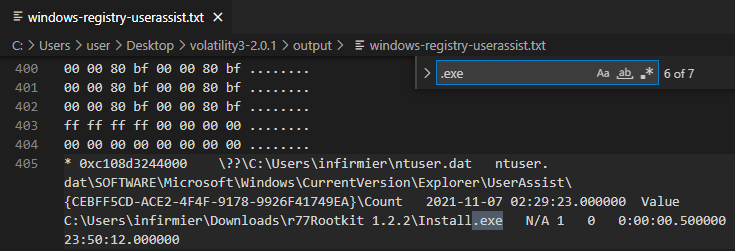
\includegraphics{images/RAM/volatility-userassist-executed-programs.png}
        }
    }
    \caption{Preuves de l'exécution d'un exécutable grâce à une clé userassist dans le registre listée avec Volatility.}
    \label{fig:volatility-userassist}
\end{figure}




% LTeX: language=fr

\chapter{Pistes d'amélioration}





\section{Analyse de malware}

Les solutions apportées en ce qui concerne l'analyse de menaces se concentre sur la mise en place d'outils d'analyse automatique dans une infrastructure isolée. Pour qu'elle soit isolée mais que le transfert de fichier reste possible, il faut passer par l'intermédiaire d'un serveur FTP, ce qui fait perdre beaucoup de temps. Cependant, en créant une ouverture firewall en HTTP uniquement pour les utilisateurs qui se connectent en VPN, il serait possible de faciliter la soumission de ces fichiers en permettant aux analystes de soumettre directement les éléments potentiellement malveillants à l'interface web de la plateforme d'analyse automatique. Il est aussi possible d'automatiser la soumission de ces fichiers pour économiser du temps. Par exemple, quand un utilisateur signale un mail comme étant potentiellement du phishing, il pourrait être automatiquement envoyé pour analyse. Ceci pourrait être fait avec la plateforme d'automatisation Splunk SOAR.

Toujours concernant l'analyse de malwares, ou plutôt l'analyse de maldocs, c'est-à-dire des documents malicieux, la machine virtuelle utilisée par le logiciel CAPE Sandbox plante lorsque l'on essaie de les lancer. Ce serait une bonne amélioration de corriger cela pour pouvoir effectuer une analyse dynamique sur ces documents. La création d'une machine virtuelle Linux pour analyser des malwares qui ne fonctionnent que sur les systèmes Linux est aussi une piste d'amélioration intéressante.

Enfin, l'analyse manuelle de logiciels malveillants pourrait aussi être approfondie. C'est une tâche qui ne sera sans doute pas effectuée tous les jours étant donné que ça pourrait faire perdre beaucoup de temps inutilement. Mais malgré tout, il faudra dans certains cas entrer plus en profondeur dans l'analyse du malware. Par exemple dans le cas où un PC a été compromis et on veut comprendre ce qu'il a fait sur le système et comment le détecter sur d'autres machines au sein de l'environnement. Approfondir les recherches sur cet aspect-là est donc une piste d'amélioration.





\section{Analyse forensique}

Pour ce qui est de l'analyse forensique, en plus d'approfondir l'analyse forensique des systèmes Windows, il est aussi possible d'étendre l'éventail des systèmes qu'on puisse analyser, comme en s'attaquant aux systèmes Linux et macOS.

Les machines d'analyse se trouvent dans un environnement virtualisé, ce qui est très pratique et flexible. Cependant, il crée également des contraintes. Par exemple, le temps de transfert des données forensiques vers l'infrastructure d'analyse peut être lent, ce qui peut faire perdre un temps crucial lors d'analyses. C'est particulièrement le cas lors d'analyses forensiques en-dehors de l'entreprise. C'est pour ça qu'avoir un PC portable pour effectuer ces analyses peut être intéressant. Il faut aussi utiliser des SSD portables, rapides et de grande capacité pour pouvoir stocker les données forensiques et les résultats d'analyse. De plus, pour analyser les clés USB, une solution de Write-Blocker physique, dans lequel on peut brancher une clé USB et ainsi empêcher l'écriture accidentelle sur la clé est un outil supplémentaire à envisager.





% LTeX: language=fr

\chapter{Conclusion}

La solution qui a été créée pourra être utilisée pour analyser les tentatives de pénétration avec des mails de phishing ou des exécutables de manière automatique. Ceci fera gagner du temps aux analystes et leur permettra de rentrer plus en profondeur dans l'analyse ce qui permet de mieux prévenir les menaces. Au niveau de l’analyse forensique des systèmes contaminés, j’ai pu répondre aux attentes en termes de procédures et de la sélection d’outils, que j’ai d’ailleurs pu tester dans des situations réelles.

Bien que les objectifs du projet aient été atteints, il reste beaucoup d'améliorations possibles à apporter et de pistes à approfondir tant au niveau de l'analyse de malware que de l'analyse forensique. Parmi les améliorations, on compte des gains de temps qui peuvent être réalisés avec encore plus d'automatisation. Ce temps libéré peut alors être utilisé afin d'étudier plus en profondeur certains cas avec une analyse manuelle plus poussée.







\appendix \renewcommand{\thechapter}{\Roman{chapter}}





\listoftables \addcontentsline{toc}{chapter}{Liste des tableaux} \newpage
\listoffigures \addcontentsline{toc}{chapter}{Table des figures} \newpage





% LTeX: language=fr

\chapter{Rapport de stage}










\section{Introduction}

Mon stage s'est passé dans l'entreprise NRB, plus précisément dans l'équipe SecOps en charge de la sécurité opérationnelle dans l'entreprise et chez plusieurs clients. Grâce à ce stage en lié au processus forensique, c'est-à-dire à l'acquisition, l'analyse des données forensique et des menaces (malware, documents malicieux, etc.), j'ai pu grandement améliorer mes connaissances en informatique et en cybersécurité.

La mise en place d'une architecture pour l'infrastructure d'analyse des données forensiques a été une première pour moi, tout comme des aspects moins techniques comme la participation à des réunions ou la gestion de projet.





\section{Objectifs du stage}

L'objectif de ce stage était de créer une solution d'analyse contenant un ensemble d'outils pour améliorer les capacités de l'équipe SecOps en termes d'analyse forensique. Ça comprend aussi la détection et l'analyse de menaces, comme les emails, les documents ou les exécutables. Cette solution doit être isolée pour éviter la propagation des menaces. Il doit aussi pouvoir être facilement restauré dans un état initial. Un ensemble d’outils de forensique et d’analyse de menaces sont utilisés comme une sandbox, des outils d'analyse réseau, des logiciels de copie et montage disque, des scripts python, etc. Le tout dans un environnement virtualisé.

La mise en place de cet environnement doit bien entendu s'accompagner de la rédaction d'une documentation pour l'utilisation et la mise à jour de l'infrastructure et des outils qu'elle contient.





\section{Présentation de l'entreprise}



\subsection{NRB}

\textit{Network Research Belgium}, souvent abrégé sous la forme du sigle \textit{NRB} est une entreprise belge du secteur des TIC, les technologies de l'information et de la communication, fondée en 1987 en Belgique mais à vocation européenne. L'entreprise fournit des services dans les quatre domaines suivants:
\begin{itemize}
    \item la \textit{consultance} pour accompagner ses clients dans leurs démarches de transformation numérique et le conseil en cybersécurité;
    \item les \textit{services logiciels} comme le développement et la maintenance d'applications;
    \item les \textit{services infrastructures et clouds}, NRB permet à ses clients d'utiliser le cloud privé de NRB et les clouds publics d'IBM, Microsoft, Google et Amazon;
    \item les \textit{services de managed staffing} consistent à fournir du personnel à des entreprises qui en ont besoin pour conduire à bien leurs projets.
\end{itemize}

Certains de ces services sont fournis par les filiales du groupe NRB. En effet, NRB est un groupe qui s'agrandit notamment par des acquisitions d'entreprises dans le domaine technologique. En 2020, le groupe NRB comptait 3200 collaborateurs, avec un chiffre d'affaires de 413 millions d'euros.



\subsection{L'équipe SecOps}

SecOps vient de \textit{Sécurité et Opérations}, c'est l'équipe principale de gestion de la sécurité chez NRB. Comme l'indique le mot \textit{sécurité} de SecOps, ils doivent gérer les incidents de sécurité qui se produisent dans l'entreprise et chez certains de leurs clients mais ils ne gèrent pas l'ensemble des \textit{opérations}. Par exemple, lorsqu'une vulnérabilité a été détectée ce n'est pas leur rôle de mettre à jour le système d'exploitation ou de patcher l'application vulnérable, c'est le rôle de l'équipe qui est responsable de cette application ou système d'exploitation. Cependant, l'équipe SecOps a la responsabilité de trouver ces vulnérabilités et de vérifier qu'elles ont bien été corrigées.

L'équipe fonctionne en mode agile ce qui fait qu'il y a deux types de charges de travail. Premièrement, il y a le \textit{build}: c'est le fonctionnement normal où chacun avance sur ses projets et améliore les outils, les procédures, participe à des réunions et améliore la sécurité de NRB et de ses clients de manière générale. Deuxièmement, il y a le \textit{run} qui est assigné à une personne qui doit résoudre les tickets assignés à SecOps comme les incidents ou bien les demandes de changements dans l'infrastructure de l'entreprise qui doivent recevoir une autorisation de sécurité pour être implémentés. Par exemple, une demande pour donner les permissions administrateur sur une machine à un utilisateur est une demande de changement et un employé recevant un mail de phishing est un incident.

Le lundi, toutes les deux semaines, l'équipe SecOps se réunit pour ce qui est appelé le \textit{sprint review} de 15h30 à 17h30. Lors de cette réunion, chaque membre de l'équipe présente ce qu'il a accompli les deux semaines précédentes et ce qu'il a prévu de faire les deux semaines suivantes. Cependant, ce n'est pas la seule réunion effectuée à intervalle régulier parce qu'il y a aussi le \textit{daily standup}, réunion journalière de 8h30 à 9h, lors de laquelle on revoit les incidents de la veille avec un dashboard et ce que chacun a prévu de faire pour la journée.





\section{Journalier}

Pendant toute la durée du stage, j'ai envoyé un rapport d'avancement de stage à mon promoteur par mail pour l'informée de l'avancement du stage, des objectifs, des problèmes rencontrés et de ce que j'ai fait au jour le jour. Le tout était accompagné d'un petit résumé pour que ce soit plus facilement lisible. Dans cette section, je vais simplifier en mettant uniquement ce résumé pour chaque semaine plutôt que d'écrire le détail de ce qui a été fait chaque jour.



\subsection{Première semaine: 31 janvier - 25 février}

Pendant la première semaine, j'ai commencé à intégrer l'équipe, à participer aux réunions, découvrir les locaux, le fonctionnement de l'organisation, etc. J'ai défini les objectifs pour le stage ainsi qu'un premier planning, notamment avec un diagramme de Gantt. J'ai aussi effectué mes premières recherches sur les sandbox, j'ai surtout essayé de lister les sandbox existantes qu'elles soient gratuites ou commerciales.



\subsection{Deuxième semaine: 7 février - 11 février}

Pendant la deuxième semaine, j'ai passé une grande partie de mon temps à lire le cours SIFR (Security Incident First Responder) d'IBM qui avait été suivie par une partie des membres de l'équipe SecOps en avril 2021. Cette formation couvre les réflexes à avoir quand il y a un incident de sécurité comme l'acquisition de données forensiques et l'analyse de malware automatiquement avec une sandbox et manuellement avec des logiciels et des scripts.



\subsection{Troisième semaine: 14 février - 18 février}

Comme prévu, lors de cette troisième semaine, j'ai passé beaucoup de temps à faire des recherches sur le processus forensique ainsi que sur les outils utilisés lors de celui-ci. À la fin de la semaine, j'ai réussi à produire un rapport sur les outils dont la connaissance est à approfondir et les distributions qui les contiennent. J'ai aussi eu l'occasion de rencontrer un client de l'entreprise.



\subsection{Quatrième semaine: 21 février - 25 février}

Cette semaine, mon maître de stage fait le \textit{run}, il doit donc s'occuper des incidents de sécurité et valider les demandes de changements dans l'infrastructure NRB qui doivent recevoir une autorisation de sécurité. J'ai donc suivi ce qu'il faisait pour voir comment tout fonctionnait et il m'a donné quelques cas simples à résoudre pour me faire la main. J'ai aussi listé les besoins en infrastructure et les outils en fonction des use cases.



\subsection{Cinquième semaine: 28 février - 4 mars}

Lors de cette cinquième semaine, j'ai revu l'infrastructure d'analyse de données forensiques et de menaces. Il faut faire attention à bien isoler les machines d'analyse parce que les malwares pourraient potentiellement les infecter et à partir de là, se répandre dans le réseau de l'entreprise. J'ai aussi continué mes recherches sur les méthodes d'analyse forensiques, notamment en étudiant la méthode utilisée par Interpol.



\subsection{Sixième semaine: 7 mars - 11 mars}

Cette semaine, je me suis concentré sur le test des différents outils d'acquisition de données forensiques listés les semaines précédentes. J'ai aussi continué les recherches sur les méthodes d'analyse forensique en me concentrant sur les preuves d'exécution d'un programme dans un environnement Windows.



\subsection{Septième semaine: 14 mars - 18 mars}

L'architecture que j'ai proposée pour les machines d'analyse a été validée. Il faut évidemment faire attention parce que si une machine d'analyse de malware est compromise, elle pourrait infecter tout le réseau et il s'agit donc de bien les isoler pour réussir à protéger l'entreprise correctement. J'ai aussi commencé à avoir accès à NECS, le cloud de NRB pour y installer l'infrastructure. Enfin, j'ai continué à faire des recherches sur l'acquisition et l'analyse de données forensiques, en particulier comment empêcher un individu malintentionné d'altérer ou supprimer les traces de ses actions.



\subsection{Huitième semaine: 21 mars - 25 mars}

J'avais commencé à installer les machines d'analyse de données forensiques et de malwares dans le cloud en fin de semaine passée et j'ai continué à le faire cette semaine. Je n'ai pas pu terminer à cause de quelques problèmes techniques : problèmes de configuration DNS et la virtualisation imbriquée qui n'est pas activée sur l'infrastructure. J'ai aussi passé les deux derniers jours de la semaine pour assister dans l'acquisition et l'analyse forensique d'un PC avec d'autres membres de l'équipe SecOps.



\subsection{Neuvième semaine: 28 mars - 1 avril}

J'ai terminé l'analyse du PC Windows 11 que j'avais commencée la semaine passée et qui a un peu décalé mon planning mais m'a permis d'apprendre beaucoup de chose et surtout de mettre en pratique mon travail. Suite à cela, j'ai écrit la marche à suivre d'acquisition de données forensique puis j'ai continué à installer l'infrastructure de sandboxing sur NECS (le cloud NRB). Ce n'est pas tout à fait terminé à cause de quelques complications pour l'activation de la virtualisation imbriquée mais le gros du travail d'installation a été effectué.



\subsection{Dixième semaine: 4 avril - 8 avril}

J'ai pu commencer à tester la virtualisation imbriquée sur NECS (le cloud NRB), ce qui est nécessaire pour utiliser CAPEv2, le logiciel d'analyse de malware. Pour tester la sandbox, j'ai commencé à écrire un petit malware mais je ne l'ai pas encore terminé parce que je passe du temps à installer la sandbox, et ce n'est pas une tâche aisée.



\subsection{Onzième semaine: 11 avril - 15 avril}

Cette semaine, j'ai réussi à installer la sandbox correctement (il y avait des problèmes de configuration) et j'ai fait des tests pour vérifier son bon fonctionnement. J'attends le retour de l'équipe VMWare cher NRB pour déplacer la sandbox du tenant de test vers le tenant de production. Les retours sont bien sûr plus lents car ce sont les vacances de Pâques. J'ai aussi effectué l'analyse forensique d'un PC Windows 10 et d'une clé USB qui avaient été compromis par un malware. Ça a permis de tester les outils forensiques dans un cas réel et de trouver des problèmes. Par exemple, à cause du changement d'heure entre le moment où le PC a été infecté et le moment de l'analyse, certains timestamps étaient mal interprétés.



\subsection{Douzième semaine: 18 avril - 22 avril}

J'ai continué à travailler sur l'installation de la sandbox et les tests pour vérifier ses capacités une fois qu'elle sera installée. J'ai eu quelques problèmes avec la virtualisation imbriquée. La semaine passée, elle avait été activée sur une VM dans le tenant de développement pour effectuer des tests et voir si elle n'affecterait pas les autres machines virtuelles de l'environnement mutualisé. Cette semaine, on l'a activée sur une machine de l'environnement de production mais pas sur la bonne. J'ai donc commencé l'installation sur l'environnement de production avec du retard. J'ai aussi créé un test pour la sandbox, c'est un fichier Excel contenant une macro exécutant des commandes powershell, déposant un exécutable sur le système. C'est difficile à analyser manuellement mais facile avec une sandbox.



\subsection{Treizième semaine: 23 avril - 27 avril}

J'ai travaillé sur l'installation d'outils supplémentaires dans les VM d'analyse et la configuration de la sandbox pour qu'elle puisse analyser des fichiers Excel (et n'importe quel document Office d'ailleurs) mais je n'ai pas réussi. Après plusieurs jours sur l'affaire en fin de semaine, j'ai dû abandonner pour continuer à avancer dans mon travail. Le mardi, on a aussi testé le Digital Escape Game créé par l'équipe SecOps pour la mission diplomatique de l'AWEX en Grèce.



\subsection{Quatorzième semaine: 2 mai - 6 mai}

J'ai terminé de travailler sur les use cases d'analyse de malware et j'ai placé l'infrastructure sur le réseau isolé (pour pouvoir effectuer des analyses de malware). Ensuite, j'ai travaillé sur la documentation et j'ai terminé la partie analyse de malware, la partie analyse forensique est toujours en cours.



\subsection{Quinzième semaine: 9 mai - 13 mai}

Cette dernière semaine de stage, j'ai retravaillé la documentation que j'avais écrite pour utiliser l'infrastructure de sandboxing et pour la mettre à jour. J'ai aussi présenté les résultats de mon stage pour montrer ce que j'avais fait à l'équipe SecOps.





\section{Autres activités réalisées}



\subsection{Suivi du run, analyse d'un cas de phishing}

Lors de la semaine de \textit{run} de mon maître de stage, je l'ai un peu suivi pour voir comment se passe la résolution de tickets dans l'équipe SecOps. J'ai ainsi pu voir comment on fait pour vérifier si un changement au niveau du pare-feu doit être autorisé ou bien refusé. Autrement dit quand accepter un changement dans l'infrastructure.

Il m'a aussi donné des cas de phishing: la plupart des mails de phishing se font arrêter à l'entrée du réseau de NRB, cependant certains passent quand même de temps à autre. L'objectif de l'équipe SecOps est alors de trouver les utilisateurs impactés pour pouvoir les prévenir de ne pas ouvrir le mail et de ne pas cliquer sur les liens présents à l'intérieur. Il faut également vérifier que personne n'a ouvert ces liens. Grâce au proxy web, on peut voir qui a ouvert quels liens et ainsi mitiger les menaces.



\subsection{Analyse d'un malware}

Le vendredi 4 mars, avec un membre de l'équipe SecOps, nous avons analysé un malware qui avait été détecté et bloqué par Windows Defender alors qu'il se trouvait dans une archive zip. Nous avons lancé une analyse statique en utilisant l'outil PeStudio. Cela nous a permis de voir les informations comme la date de compilation qui aurait été réalisée en 2096... En observant le reste des propriétés statiques, force est de constater que le malware est obfusqué, c'est-à-dire qu'il cache une partie de son code et le chargera lui-même au moment de l'exécution pour empêcher ou tout du moins compliquer l'analyse statique.

Après avoir copié son hash sur \textit{virustotal} et des sandboxes gratuites en ligne comme \textit{any.run}, nous avons pu observer que ce malware avait déjà été soumis sur ces sites en 2019. Grâce à l'analyse dynamique fournie par ces services, nous savons qu'il lance un autre processus en utilisant \textit{rundll32.exe}, c'est une technique populaire des auteurs de malwares pour donner l'impression que leur processus est légitime, car bien que la librairie exécutée est la leur, le processus est lancé avec un exécutable Windows. Ce cheval de Troie va également chercher les adresses IP de deux domaines et les contacter. Tous ces indicateurs de compromissions sont utiles pour vérifier qu'aucune machine dans le parc informatique n'a été infectée.



\subsection{Analyse forensique d'un PC Windows}

Fin mars, l'équipe SecOps de NRB a eu un cas où elle devait analyser un PC Windows 11 pour essayer de comprendre un incident. J'ai eu la chance de pouvoir y participer et tester les outils que j'avais sélectionnés. Après avoir fait une capture RAM avec \textit{Belkasoft RAM Capturer}, j'ai enchaîné avec une image disque à l'aide de \textit{FTK Imager}.

Une fois l'acquisition des données forensiques effectuée, il a fallu lancer quelques programmes utilisés pour la réponse à incident comme \textit{Process Explorer} et \textit{Autoruns} de la suite d'outils de \textit{Sysinternals} (voir figures \ref{fig:autoruns} et \ref{fig:process-explorer}). En analysant un par un les processus en train de tourner et les traces de persistance sur l'ordinateur, on peut espérer retrouver un malware qui tourne ou aurait tourné sur la machine.

Finalement, j'ai analysé les données forensiques avec \textit{Autopsy} et \textit{Volatility 3}. Comme les disques étaient chiffrés avec BitLocker (une technologie Microsoft de chiffrement de disque dur), il a fallu monter l'image disque en lecture seule sur le PC d'analyse avec \textit{Arsenal Image Mounter}. On peut ensuite déchiffrer les disques avec les clés BitLocker récupérées préalablement sur l'ordinateur et analyser le disque déchiffré dans Autopsy.

\begin{figure}
    \centering
    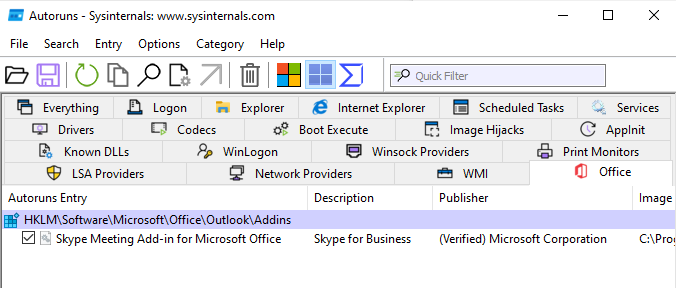
\includegraphics[width=0.75\linewidth]{images/incident-response/IR-autoruns.png}
    \caption{Logiciel \textit{Autoruns} de la suite \textit{Sysinternals} utilisé dans le cadre d'une réponse à incident.}
    \label{fig:autoruns}
\end{figure}

\begin{figure}
    \centering
    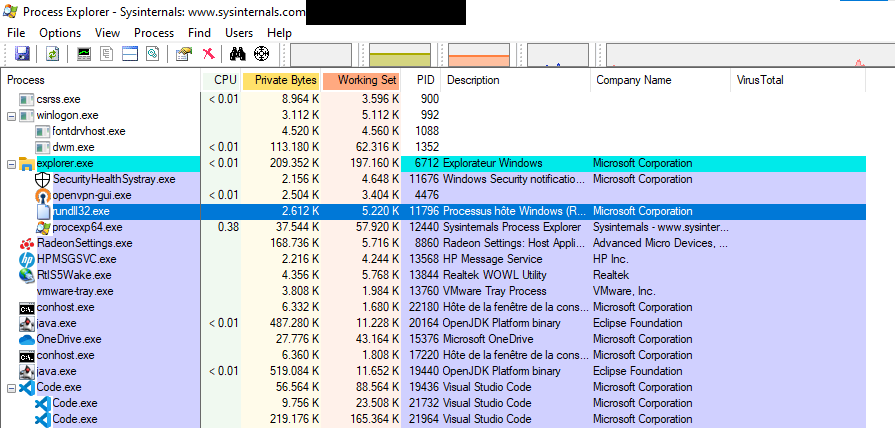
\includegraphics[width=0.99\linewidth]{images/incident-response/IR-process-explorer.png}
    \caption{Logiciel \textit{Process Explorer} de la suite \textit{Sysinternals} utilisé dans le cadre d'une réponse à incident.}
    \label{fig:process-explorer}
\end{figure}



\subsection{Analyse d'une clé USB infectée}

Mi-avril, j'ai eu l'occasion d'analyser une clé USB infectée. Le fonctionnement du malware est intéressant parce qu'il est simple et efficace. Quand on branche la clé sur le PC, l'explorateur de fichiers s'ouvre sur la racine du système de fichiers qui ne contient qu'un "Lecteur USB" comme vous pouvez le voir sur la figure \ref{fig:infected-usb-key}. En fait, il s'agit d'un raccourci qui exécute un script caché. Ce script lance l'installation d'un malware et ouvre une nouvelle fenêtre explorer dans le dossier caché \textit{Lecteur USB} pour tromper l'utilisateur.

Bien que les options pour afficher les extensions de noms de fichiers et les éléments masqués soient sélectionnées, on ne voit ni l'extension du raccourci, ni les éléments masqués. C'est parce qu'en plus d'avoir l'attribut \textit{Hidden}, les éléments cachés ont l'attribut \textit{System} qui n'est normalement possédé que par des fichiers et dossiers nécessaires au bon fonctionnement de Windows. Le paramètre pour les afficher malgré tout se trouve dans le \textit{Control Panel}.

\begin{figure}
    \centering
    \makebox[\textwidth]{
        \resizebox{17cm}{!}{
            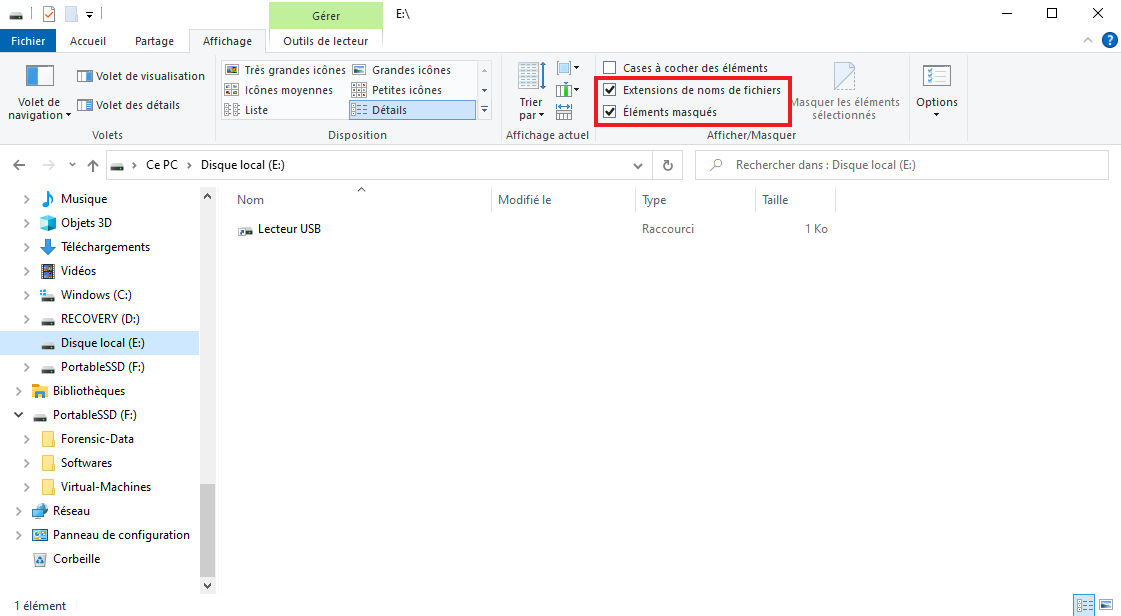
\includegraphics[width=0.99\linewidth]{images/infected-usb-key/explorer-listing.png}
        }
    }
    \caption{Racine de la clé USB infectée dans l'explorateur de fichiers.}
    \label{fig:infected-usb-key}
\end{figure}

Après avoir effectué une image disque de la clé USB, j'ai lancé une analyse avec le logiciel Autopsy qui a scanné l'ensemble de l'image et retrouvé des éléments supprimés. En fait, parce que le système de fichier est du FAT32, quand on déplace un dossier, il est supprimé et recréé à cet autre endroit. On peut le voir sur la figure \ref{fig:autopsy-moved-folders}, où le dossier \textit{Documents} a été déplacé de la racine du système de fichier vers l'intérieur du dossier \textit{Lecteur USB}. Dans ce cas-ci, c'est très intéressant parce que ça nous informe que:
\begin{itemize}
    \item La clé USB était utilisée normalement auparavant.
    \item Elle a été infectée par un PC qui appartient sans doute à la victime.
    \item Donc l'infection du PC est potentiellement antérieure à l'infection de la clé.
\end{itemize}

\begin{figure}
    \centering
    \makebox[\textwidth]{
        \resizebox{10cm}{!}{
            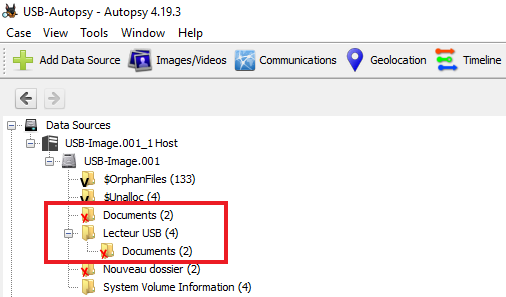
\includegraphics[width=0.99\linewidth]{images/infected-usb-key/autopsy-moved-folders.png}
        }
    }
    \caption{Analyse d'un déplacement de dossier sur la clé USB.}
    \label{fig:autopsy-moved-folders}
\end{figure}





\section{Résultats}

J'ai décidé de diviser cette section en deux parties: l'analyse de malware et l'analyse forensique. Bien que l'analyse de malware fasse partie de l'analyse forensique et que les solutions aux deux problèmes soient liées, il y a eu un grand effort pour travailler ce sujet lors du TFE et je pense donc que c'est plus intéressant de séparer les résultats ici.



\subsection{Analyse de malware}

L'analyse de malware peut être réalisée de manière automatique avec la plateforme d'analyse automatique FAME qui a été mise en place, ainsi que la sandbox. On peut y mettre des emails, des documents, des exécutables et encore d'autres types de fichiers. Il y a cependant des problèmes avec l'analyse automatique dynamique des documents Office avec la sandbox parce que la machine virtuelle imbriquée, infectée volontairement pour monitorer le document, plante complètement. Malgré ces soucis, on peut tout de même tout analyser, y compris les documents Office, avec la plateforme d'analyse automatique FAME. Les analyses effectuées sur ces documents ne pourront cependant être que statiques et pas dynamiques.

En plus de la sélection des outils et de leur mise en place, une infrastructure a été pensée pour isoler les machines virtuelles d'analyse et de la documentation a été écrite pour pouvoir mettre à jour les outils et les utiliser. Ces outils et ces marches à suivre ont été testés sur plusieurs use cases et avec des cas concrets par moi-même et plusieurs membres de l'équipe SecOps.



\subsection{Acquisition et analyse forensique}

Cette section s'appelle \textit{acquisition et analyse forensique} parce que j'ai sélectionné et installer des logiciels d'acquisition des données forensiques comme la mémoire volatile et la mémoire de masse et parce que j'ai aussi effectué des recherches sur les outils et les procédures d'analyse de ces données. Pour que les procédures puissent être suivies par d'autres membres de l'équipe SecOps à l'avenir, j'ai écrit de la documentation sur l'utilisation de tous ces outils et les informations intéressantes qui peuvent en être extraites.

J'ai eu la chance lors de ce stage d'avoir pu participer à deux enquêtes forensiques sur des systèmes Windows et une clé USB avec d'autres membres de l'équipe SecOps, ce qui a été très enrichissant tant d'un point de vue social que technique. Par ces occasions, j'ai pu confronter les outils et les procédures d'acquisition et d'analyse forensique à la réalité et ne pas rester uniquement dans la théorie.





\section{Améliorations possibles}



\subsection{Analyse de malware}

L'apport de ce stage concernant l'analyse de malwares est principalement concentré sur la mise en place d'outils d'analyse automatique dans une infrastructure isolée. Et parce que l'infrastructure est isolée, c'est plus difficile de déplacer des fichiers à analyser du PC de l'analyste vers la machine virtuelle d'analyse. Ainsi, on pourrait pousser l'automatisation encore plus loin en soumettant automatiquement des éléments potentiellement malveillants ce qui ferait gagner du temps aux analystes. Après discussion avec des membres de l'équipe SecOps, ça pourrait être fait avec la plateforme d'automatisation Splunk SOAR.

Toujours concernant l'analyse de malwares, ou plutôt l'analyse de maldocs, c'est-à-dire des documents malicieux, la machine virtuelle utilisée par le logiciel CAPE Sandbox plante lorsqu'on essaie de les lancer. Ce serait une bonne amélioration de corriger cela pour pouvoir effectuer une analyse dynamique sur ces documents. La création d'une machine virtuelle Linux pour analyser des malwares qui ne fonctionnent que sur les systèmes Linux est aussi une piste d'amélioration intéressante.

Enfin, l'analyse manuelle de logiciels malveillants pourrait aussi être approfondie. C'est une tâche qui ne sera sans doute pas effectuée tous les jours étant donné que ça pourrait faire perdre beaucoup de temps inutilement. Mais malgré tout, il faudra dans certains cas entrer plus en profondeur dans l'analyse du malware. Par exemple dans le cas où un PC a été compromis et on veut comprendre ce qu'il a fait sur le système et comment le détecter sur d'autres machines au sein de l'environnement. Travailler plus cet aspect-là peut donc être intéressant.



\subsection{Analyse forensique}

Pour ce qui est de l'analyse forensique, en plus d'approfondir l'analyse forensique des systèmes Windows, il est aussi possible d'étendre l'éventail des systèmes qu'on peut analyser comme en s'attaquant aux systèmes Linux et macOS.

Les machines d'analyse se trouvent dans un environnement virtualisé, ce qui est très pratique et flexible. Cependant, il crée également des contraintes. Par exemple, le temps de transfert des données forensiques vers l'infrastructure d'analyse peut être lent, ce qui peut faire perdre un temps crucial lors d'analyses, particulièrement en-dehors de l'entreprise. C'est pour ça qu'avoir un PC portable pour effectuer des analyses forensiques peut être intéressant. Il faut aussi utiliser des SSD portables, rapides et de grande capacité pour pouvoir stocker les données forensiques et les résultats d'analyse. De plus, pour analyser les clés USB, une solution de Write-Blocker physique, dans lequel on peut brancher une clé USB et ainsi empêcher l'écriture accidentelle sur la clé est un outil supplémentaire à envisager.





\section{Diagrammes de Gantt}

Comme vous pouvez le voir, au début, j'avais des difficultés à réaliser mon premier diagramme de Gantt. D'abord, c'était la première fois que je me prêtais à cet exercice mais je manquais aussi d'informations pour que le diagramme de Gantt soit précis. J'ai donc laissé certaines tâches globales pendant plusieurs semaines plutôt que de les rediviser en plus petites tâches. En présentant ce planning à mon maître de stage, mais aussi à l'équipe SecOps en entier lors d'une réunion de sprint review, j'ai pu avoir des retours. Ça m'a aidé à mieux cerner le but du stage et modifier ce que j'avais prévu de faire pour m'aligner sur ces objectifs.

Lorsque j'ai à nouveau créé un diagramme de Gantt, en milieu de stage, une partie du stage avait déjà été réalisée et la roadmap était beaucoup plus claire dans mon esprit. Grâce à ce nouveau diagramme, j'ai pu à nouveau communiquer. Cette fois, c'était surtout avec mon maître de stage pour valider les priorités et s'assurer que les objectifs du stage puissent être atteints.

Enfin, le dernier diagramme de Gantt permet surtout de faire le point sur ce qui a été fait, identifier avec du recul les tâches qui ont pris le plus de temps et revoir les points bloquants qui ont ralenti la progression du travail.

\begin{figure}
    \centering
    \noindent
    \makebox[\textwidth]{
        \resizebox{19cm}{!}{
            \includestandalone{images/gantt-chart/gantt-chart}
        }
    }
    \caption{Diagrammes de Gantt réalisés à différentes périodes du stage.}
    \label{fig:gantt-diagrams}
\end{figure}





\section{On Stage}

\begin{figure}
    \centering
    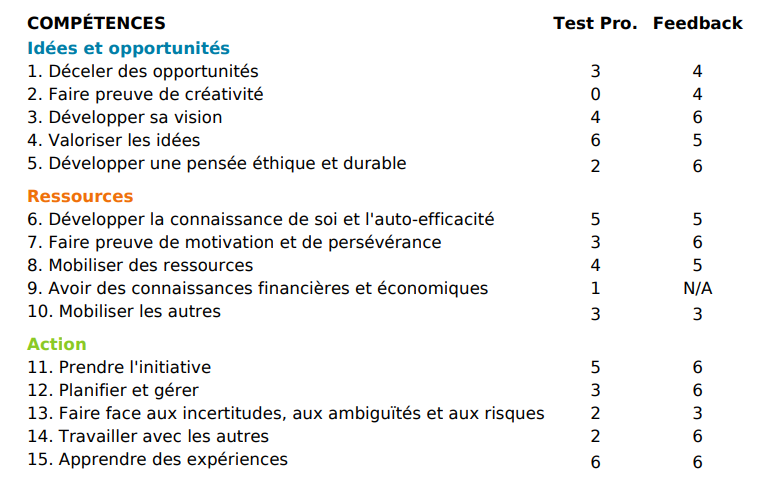
\includegraphics[width=0.85\linewidth]{images/onstage/onstage-skills.png}
    \caption{Résultats de la plateforme On Stage.}
    \label{fig:onstage}
\end{figure}

Comme vous pouvez le voir sur la figure \ref{fig:onstage}, parmis mes points faibles, il y a se confronter aux incertitudes, les connaissances financières et économiques, ainsi que mobiliser les autres. Mes points forts se trouvent plutôt dans la section \textit{Action}, par exemple: apprendre de mes expériences, travailler avec les autres, la planification.





\section{Critique du stage}

Grâce à ce stage, j'ai maintenant une meilleure compréhension du monde professionnel et du fonctionnement des grandes entreprises mais aussi de l'importance de la cybersécurité dans ce milieu et comment la mettre en place. J'ai aussi pu acquérir de nombreuses compétences en informatique et plus spécifiquement en termes de forensique, d'analyse de malware et en architecture de solutions.

La solution que j'ai apportée à l'entreprise pourra être utilisée pour analyser les tentatives de pénétration avec des mails de phishing ou des exécutables de manière automatique, ce qui fera gagner du temps aux analystes et leur permettra de rentrer plus en profondeur pour mieux prévenir les menaces. Au niveau de l'analyse forensique des systèmes contaminés, j'ai pu répondre aux attentes en termes de procédures et de la sélection d'outils, que j'ai d'ailleurs pu tester dans des situations réelles.

J'ai rencontré un point négatif, comme c'est souvent le cas dans une grande entreprise, on est dépendant d'autres équipes. Ça a ralenti la progression du travail, notamment quand on doit faire travailler plusieurs équipes ensemble et qu'il faut trouver un moment de libre pour amener tout le monde ensemble dans une réunion.

En revanche, l'avantage de faire de la cybersécurité dans une grande entreprise est qu'on peut avoir l'opportunité de communiquer avec beaucoup de personnes et de toucher à beaucoup de technologies. Un autre avantage, c'est que l'équipe SecOps est elle est plutôt jeune et dynamique. Elle est en pleine croissance et il y a toujours beaucoup de choses à faire et à entreprendre.





\section{Conclusion}

Ce stage m'a beaucoup apporté et a été une expérience professionnelle très enrichissante. Il m'a permis d'en apprendre beaucoup plus d'un point de vue technique bien entendu, surtout dans le domaine de la forensique, de l'analyse de malware ou plus généralement dans le fonctionnent de Windows. Mais j'ai aussi retenu des leçons sur l'organisation: lister les objectifs à atteindre, créer une liste de tâches pour les atteindre et estimer le temps que chacune va prendre. Ensuite, en communiquant avec d'autres personnes, on peut avoir un retour et corriger le planning. C'est d'ailleurs quelque chose qu'il faut faire régulièrement pour résoudre les problèmes qui vont invariablement arriver et réorienter le travail pour atteindre les objectifs.

D'ailleurs, en faisant ce stage, j'ai mieux compris à quel point la communication était importante. En particulier, parce que NRB est une grande entreprise, elle est divisée en plusieurs plus petites équipes et j'ai dû interagir avec certaines d'entre elles pour pouvoir accomplir mes tâches. J'ai aussi eu l'occasion de travailler avec des clients. Et bien sûr, j'ai beaucoup communiqué avec le reste de l'équipe. D'abord lors des réunions qui étaient organisées tous les jours mais aussi en dehors.








\begin{thebibliography}{9} \addcontentsline{toc}{chapter}{Bibliographie}
    \bibitem{1} \textit{Cybersecurity Incident - Glossary}. (s. d.). NIST Computer Security Resource Center. Consulté le 31 mars 2022, à l’adresse \url{https://csrc.nist.gov/glossary/term/cybersecurity\_incident}
    \bibitem{2} National Institute of Standards and Technology (2012) \textit{Computer Security Incident Handling Guide}. (Department of Commerce, Washington, D.C.), NIST Special Publication 800-61 Revision 2. \url{http://dx.doi.org/10.6028/NIST.SP.800-61r2}
    \bibitem{3} \textit{Digital forensics}. (s. d.). Interpol. Consulté le 3 avril 2022, à l’adresse \url{https://www.interpol.int/How-we-work/Innovation/Digital-forensics}
    \bibitem{4} Interpol (2019) \textit{INTERPOL Global guidelines for digital forensics laboratories}.
    \bibitem{5} National Institute of Standards and Technology (2006) \textit{Guide to Integrating Forensic Techniques into Incident Response}. (Department of Commerce, Washington, D.C.), NIST Special Publication 800-86. \url{https://doi.org/10.6028/NIST.SP.800-86}
    \bibitem{6} Association of Chief Police Officers (2011) \textit{Good Practice Guide for Digital Evidence}.
    \bibitem{7} \textit{Mémoire virtuelle}. (s.d.). Wikipedia. Consulté le 19 avril 2022, ) l'adresse \url{https://fr.wikipedia.org/wiki/M\%C3\%A9moire_virtuelle}
    \bibitem{8} \textit{Volatility Framework}. (s. d.). GitHub. Consulté le 19 avril 2022, à l’adresse \url{https://github.com/volatilityfoundation/volatility3/blob/7626f60bb494d11ad29b7073bbbb5a95f16c98a9/volatility3/framework/exceptions.py\#L55}
    \bibitem{9} \textit{Comparison of Memory Acquisition Software for Windows}. (2021, 25 décembre). Medium. Consulté le 24 avril 2022, à l’adresse \url{https://thanursan.medium.com/comparison-of-memory-acquisition-software-for-windows-e8c6d981db23}
    \bibitem{10} \textit{Process Injection : Process Hollowing, Sub-technique T1055.012}. (s. d.). Mitre. Consulté le 30 avril 2022, à l’adresse \url{https://attack.mitre.org/techniques/T1055/012/}
    \bibitem{11} \textit{Get Bitlocker Recovery Key From Cmd}. (s. d.). Password Recovery. Consulté le 29 mars 2022, à l’adresse \url{https://www.top-password.com/blog/tag/get-bitlocker-recovery-key-from-cmd/}
    \bibitem{12} \textit{Make USB Storage Read-Only : Registry, Group Policy, or Software}. (2012, 19 juillet). SumTips. Consulté le 29 mars 2022, à l’adresse \url{https://sumtips.com/how-to/make-usb-storage-read-only-registry-group-policy-or-software/}
    \bibitem{13} \textit{Finding Advanced Malware Using Volatility}. (2016, 29 juin). eForensics. Consulté le 3 mars 2022, à l’adresse \url{https://eforensicsmag.com/finding-advanced-malware-using-volatility/}
\end{thebibliography}










\end{document}
